%=========================================================================

%- potreba mit 10-20 vysazenych stran / 20-40 normostran
%- na jednu plne potistenou stranu se vleze 1,65 (s nadpisem chapter) nebo 2,36 (bez nadpisu) normostran

% Setting the depth of sections numbering
\setcounter{secnumdepth}{2}
% Setting the depth of sections to appear in the table of contents.
\addtocontents{toc}{\protect\setcounter{tocdepth}{1}}


%=========================================================================
%=========================================================================
\chapter{Introduction} \label{txt:introduction}

An autonomous localization of arbitrary moving targets is an essential system component used in multiple domains, such as air traffic control, robotic workspaces or surveillance and defense systems. If the sensory data measured by the target are available it is straightforward to derive its location (by means of the GPS, radio multilateration, etc.). There are scenarios, however, were the target is unable (malfunctioning aircraft) or reluctant (UAV intruder) to expose its location. Then the localization estimation system is left with its own observations.  Among others, nowadays, the air traffic control (ATC) and national defense systems are the most widely used applications of tracking and localizing the moving objects. 

In case of the ATC, the airports mainly rely on the multilateration systems which specialize on surveillance and control of air traffic during all flight phases \cite{Gaviria:newStrategiesMLAT}. The design of such a system expects that the aircraft are equipped with a secondary surveillance radar transponders which periodically emit the signals to the ground receiving stations, however, primary radars are widely used as well \cite{Airtrafficmuseum}. 

In the military segment the object localization mainly serves the purpose of the early threat detection where it is necessary to identify and track the intruder which might pose a threat for a given area under protection. In this scenario only primary radars are used since the objects of interest are not expected to cooperate.

Besides the ATC and the national defense there are quite a lot other use cases where the autonomous localization systems are or could be employed. The road traffic security is one of such examples. The localization systems can be used by the police to measure the speed of vehicles and prospectively to pinpoint the exact locations where the speeding occurred. Autonomous traffic analysis is another well suited application for localization systems as the main requirement estimate the tracks of given vehicles with regards to the underlying geographical map.

Even though being widely used, radar based localization systems suffer from several drawbacks. Radar is a device based on the active emission of the radio signal \cite{toomay2012radar}. In order to localize distant objects, a huge amount of energy must be radiated to make sure it would return from the target and a small amount of energy returned might be easily disrupted \cite{Airtrafficmuseum}. What is more, in defense applications it is not desirable that the tracked object would find out that it is being tracked, which is the condition an actively radiating system, such as a radar, cannot achieve. Last but not least, the professional class radars in use by both public segment and military are in general expensive, large and heavy devices not suitable for mobile deployment.

This work presents a semi-autonomous passive multi-camera system for tracking and localizing arbitrary objects --- the Optical Localization System (OLS) --- which is based merely on ordinary RGB cameras. Since the system does not rely on active emission of a signal but rather captures the optical information from the environment, it can be used for secret localization of moving targets. The system is designed to be well suited for mobility and temporary deployment since each camera station used weigh no more than twenty kilograms and the whole system is inexpensive by comparison to radars as well.

The principle of the optical localization of objects, which is based on triangulation, is well known for quite a long time. The first devices which were designed to allow an operator to estimate a distance to a given object using mechanical and optical principles --- optical range finders --- emerged in the second half of the 18th century \cite{bud1998instruments}. Ever since, the optical range finders had been mostly used for military operations in order to estimate the position of either naval, airborne or terrestrial targets until the World War II when radar was invented.

The OLS aims to utilize the same principle as the old optical range finders. However, instead of an optical device requiring the operator to aim on the target manually the OLS takes advantage of the RGB cameras and the image processing techniques capable of tracking and localizing the target autonomously without the need for a human to interfere. Furthermore, with the use of sensors capable of finding a geographical position of each observing unit the OLS system estimates a global geographical position of a given target represented in standard coordinate system (UTM and/or WGS84). A simple schema explaining the operation of the OLS is depicted in Figure \ref{fig:ols_principle}.

This work is organized as follows: In Chapter \ref{txt:related_work} the existing approaches to visual tracking, multi-camera target localization and 3D environment reconstruction are summarized and their suitability for the OLS is discussed. Chapter \ref{txt:precision_of_the_localization} provides thorough analysis of the main sources of localization imprecisions in the OLS and proposes the methods to alleviate the error. Chapter \ref{txt:design_of_the_OLS} describes the design of the OLS from the perspective of system model, visual tracking, triangulation with noisy measurements and occlusion prediction. Chapter \ref{txt:implementation} explains the technical details of the implementation and Chapter \ref{txt:experimental_results} presents the results of conducted experiments. Finally, Chapter \ref{txt:conclusion} concludes the work.

%% The main principle of the OLS.
\begin{figure}[htb]\centering
	\centering
	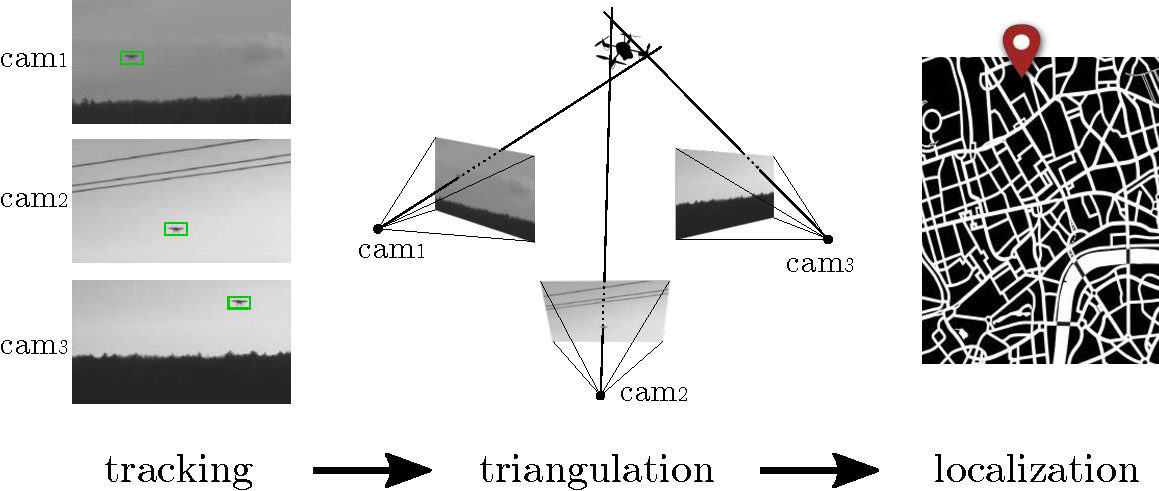
\includegraphics[width=0.8\linewidth]{fig/ols_principle.pdf}
	\caption{In the OLS a target is tracked by multiple cameras and triangulation is used in order to estimate its global location.}
	\label{fig:ols_principle}
\end{figure}

%=========================================================================
%=========================================================================
\chapter{Related Work} \label{txt:related_work}

Being a complex and semi-autonomously working system the multi-camera optical localization system comprises problematics ranging over several different areas. Most importantly, robust visual tracking capable of long-term tracking of arbitrary target which might exhibit time varying appearance and which might move in a cluttered environment must be employed. Furthermore, a suitable approach for estimating the position of the target in 3-space given noisy measurements must be proposed. Finally, occlusion prediction using 3D environment reconstruction can ne incorporated as a possible extension. The overview of visual tracking approaches and the discussion of their suitability for the OLS is given in Section~\ref{txt:object_tracking}, the most widely used methods for localizing targets in 3-space given projective geometry are described in Section~\ref{txt:multi_camera_target_localization} and the problematics of 3D environment reconstruction is introduced in Section~\ref{txt:3d_environment_reconstruction}.

%-------------------------------------------------------------------------
%-------------------------------------------------------------------------
%\section{Moving Object Detection}
%
%Before a tracking of the object can be initiated, the object of interest must first be discovered, which is the main task of object detectors. Even though the OLS allows a human operator to interfere and manually select an object for tracking, the system should be able to perform fully autonomously as well. The approaches to detect an object can be divided into two categories based on the appearance of the object, where the first group covers the cases where the system already posses a strong information about the objects since they incorporate artificial landmarks, while the second group relies merely on the natural appearance and has only limited or no prior knowledge about the objects \cite{Multi-Camera_Sensor_System_for_3D_Segmentation}. Since the OLS aims on tracking unknown UAVs the first group of approaches is out of question.
%
%A couple of approaches can be distinguished among the detectors using natural appearance \cite{Yilmaz:2006:OTS:1177352.1177355}:
%
%\paragraph{detection of points} This approach goes with the shape representation of the object given by the keypoints. Among others the Harris corner detector or SIFT and SURF descriptors are widely used.
%
%\paragraph{background modeling} Under the assumption an observed scene does not change rapidly its appearance can be learned resulting in a background model. The task of the object detector is then to estimate for each subregion or even each pixel whether it belongs to a background or to a foreground (i.e. the object of interest). A widely used approach is to model each pixel as a mixture of Gaussians (in order to support a periodically changing background). Another possible solution is to model intensity variations of separate pixels as the states (including both \textit{background} and \textit{foreground} state) and then with the help of Hidden Markov Models to estimate the state a given pixel is currently in. Since it is possible to enhance these algorithms to allow for the camera motion (resulting in the change of the camera view) they seem suitable for the OLS system. 
%
%\paragraph{supervised classification} If the (coarse) class of the objects to be tracked is known beforehand and a proper dataset is available, a classifier can be trained to detect the objects. Among others, the neural networks or adaptive boosting methods are widely used. Since the OLS aims to localize UAVs, the utilization of a classifier seems like a suitable solution.

%-------------------------------------------------------------------------
%-------------------------------------------------------------------------
\section{Object Tracking} \label{txt:object_tracking}

This section discusses the various approaches to tracking of the objects using the computer vision techniques. First, the importance of the suitable object representation is explained and the properties of various object models as well as their advantages and disadvantages with regards to the requirements of the OLS system are discussed. Different categories of tracking algorithms are then described and two specific approaches which are most appropriate for the OLS -- the \textit{TLD tracker} and the \textit{BGFG tracker based on the particle filter framework} -- are explained in more detail.

%.........................................................................
%.........................................................................
\subsection{Object Model} \label{txt:object_model}

The choice of how the targets are represented determines the domain of approaches used for visual tracking due to the strong relationship between the algorithm and the object model. Neither of the stat-of-the-art approaches is universal enough to cope with all the difficulties and disturbances, such as the illumination change, occlusion, cluttered background, motion blurring or appearance change due to deformation and/or transformation of the object \cite{Li:2013:SAM:2508037.2508039} which might occur over the course of tracking. Therefore, the model should suit a priori known tracking conditions (e.g. size, speed, rigidity and motion model of the target, number of targets, camera motion, background model etc.). Yilmaz et al. classified the model representations into two categories in their review \cite{Yilmaz:2006:OTS:1177352.1177355} -- the \textit{shape} and the \textit{appearance}. 

%Beyond these two classes, a few categories of widely used image features can be distinguished, e.g. \textit{gradient, texture or spatio-temporal features}, with some of them being specifically developed for tracking certain classes of objects, such as pedestrians or cars \cite{Yang20113823}.

\paragraph{shape representation} 
A \textit{shape} model encompasses points \cite{Tomasi91detectionand}, contours \cite{Kass88snakes:active, ActiveContour-BasedVisualTracking} or articulated models \cite{Delamarre2001328, conf/isvc/MigniotA13} (see Figure \ref{fig:object_models}). The point representation is not suitable for the OLS since the distant objects appear relatively small in the image and might not provide enough distinctive points (see Figure \ref{fig:two_small_tracked_objects}). Both contours and articulated models are mostly used for tracking non-rigid deformable objects which is not the main concern of the OLS. Additionally, the accuracy of fitting a contour to a target strongly depends on the convergence criteria of the energy minimization function, thus they might be computationally expensive.

%% Two images of distant targets which appear small in the image - an UAV and a person.
\begin{figure}[htb]\centering
	\centering
	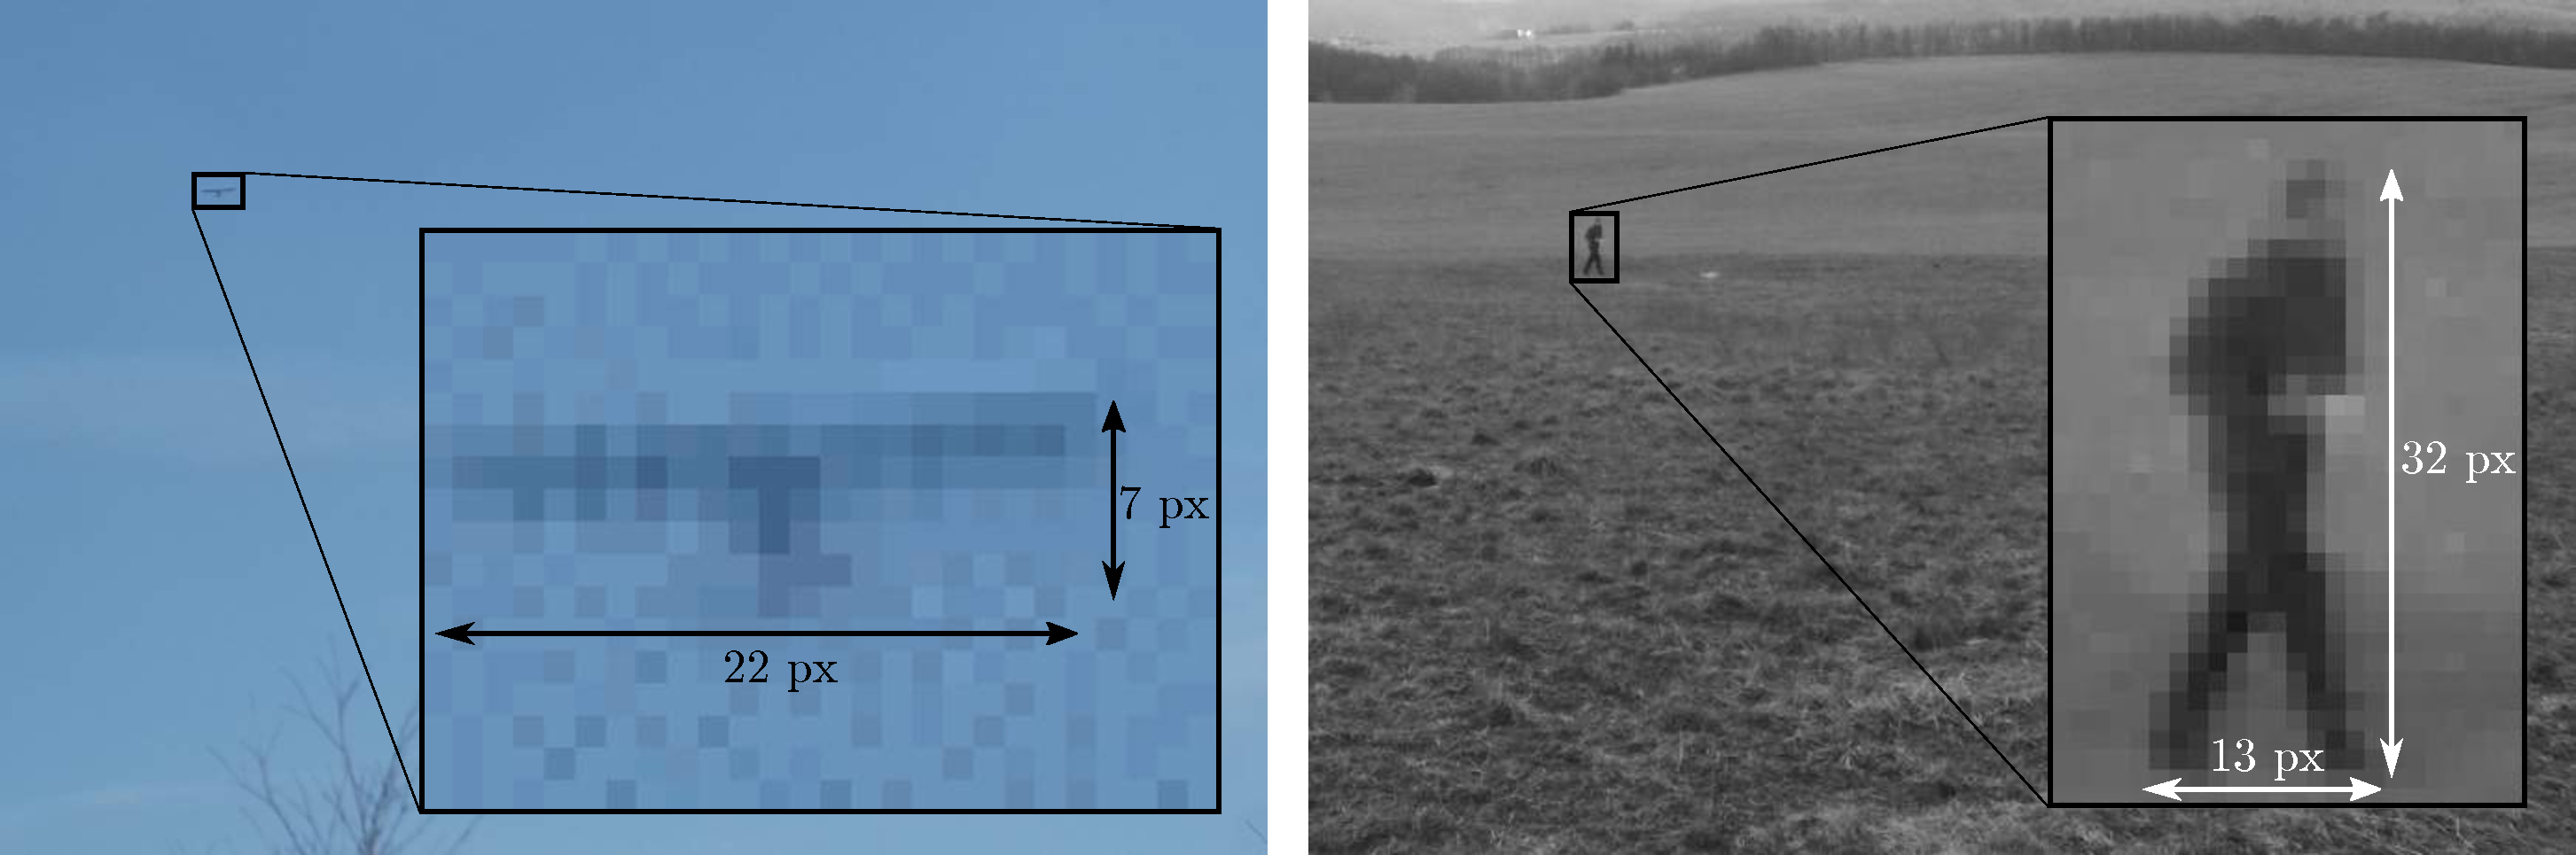
\includegraphics[width=0.7\linewidth]{fig/two_small_tracked_objects.pdf}
	\caption{Due to their high distance the tracked objects might appear small as projected to the image plane. Therefore, a suitable object model must be chosen to avoid tracking failures.}
	\label{fig:two_small_tracked_objects}
\end{figure}

\paragraph{appearance representation} 
An \textit{appearance} model is represented either by rectangular template \cite{ProbabilisticVisualTrackingTemplate, ObjectTrackinginMonochromaticVideo} or a weighted kernel \cite{Comaniciu:2003:KOT:776753.776799, MultipleCollaborativeKernelTracking} (see Figure \ref{fig:object_models}). The main advantage of both representations is the fact they contain both the spatial and appearance information, additionally they scale well to varying object size (approaching and receding object). The appearance model seem to suit the requirements of the OLS, thus the tracking approaches based on variants of both template and kernel model will be used (see Sections \ref{txt:tracking_learning_detection} and \ref{txt:bgfg_tracker}).

%% Object models - shape and appearance representation.
\begin{figure}[tbh]
	\centering
	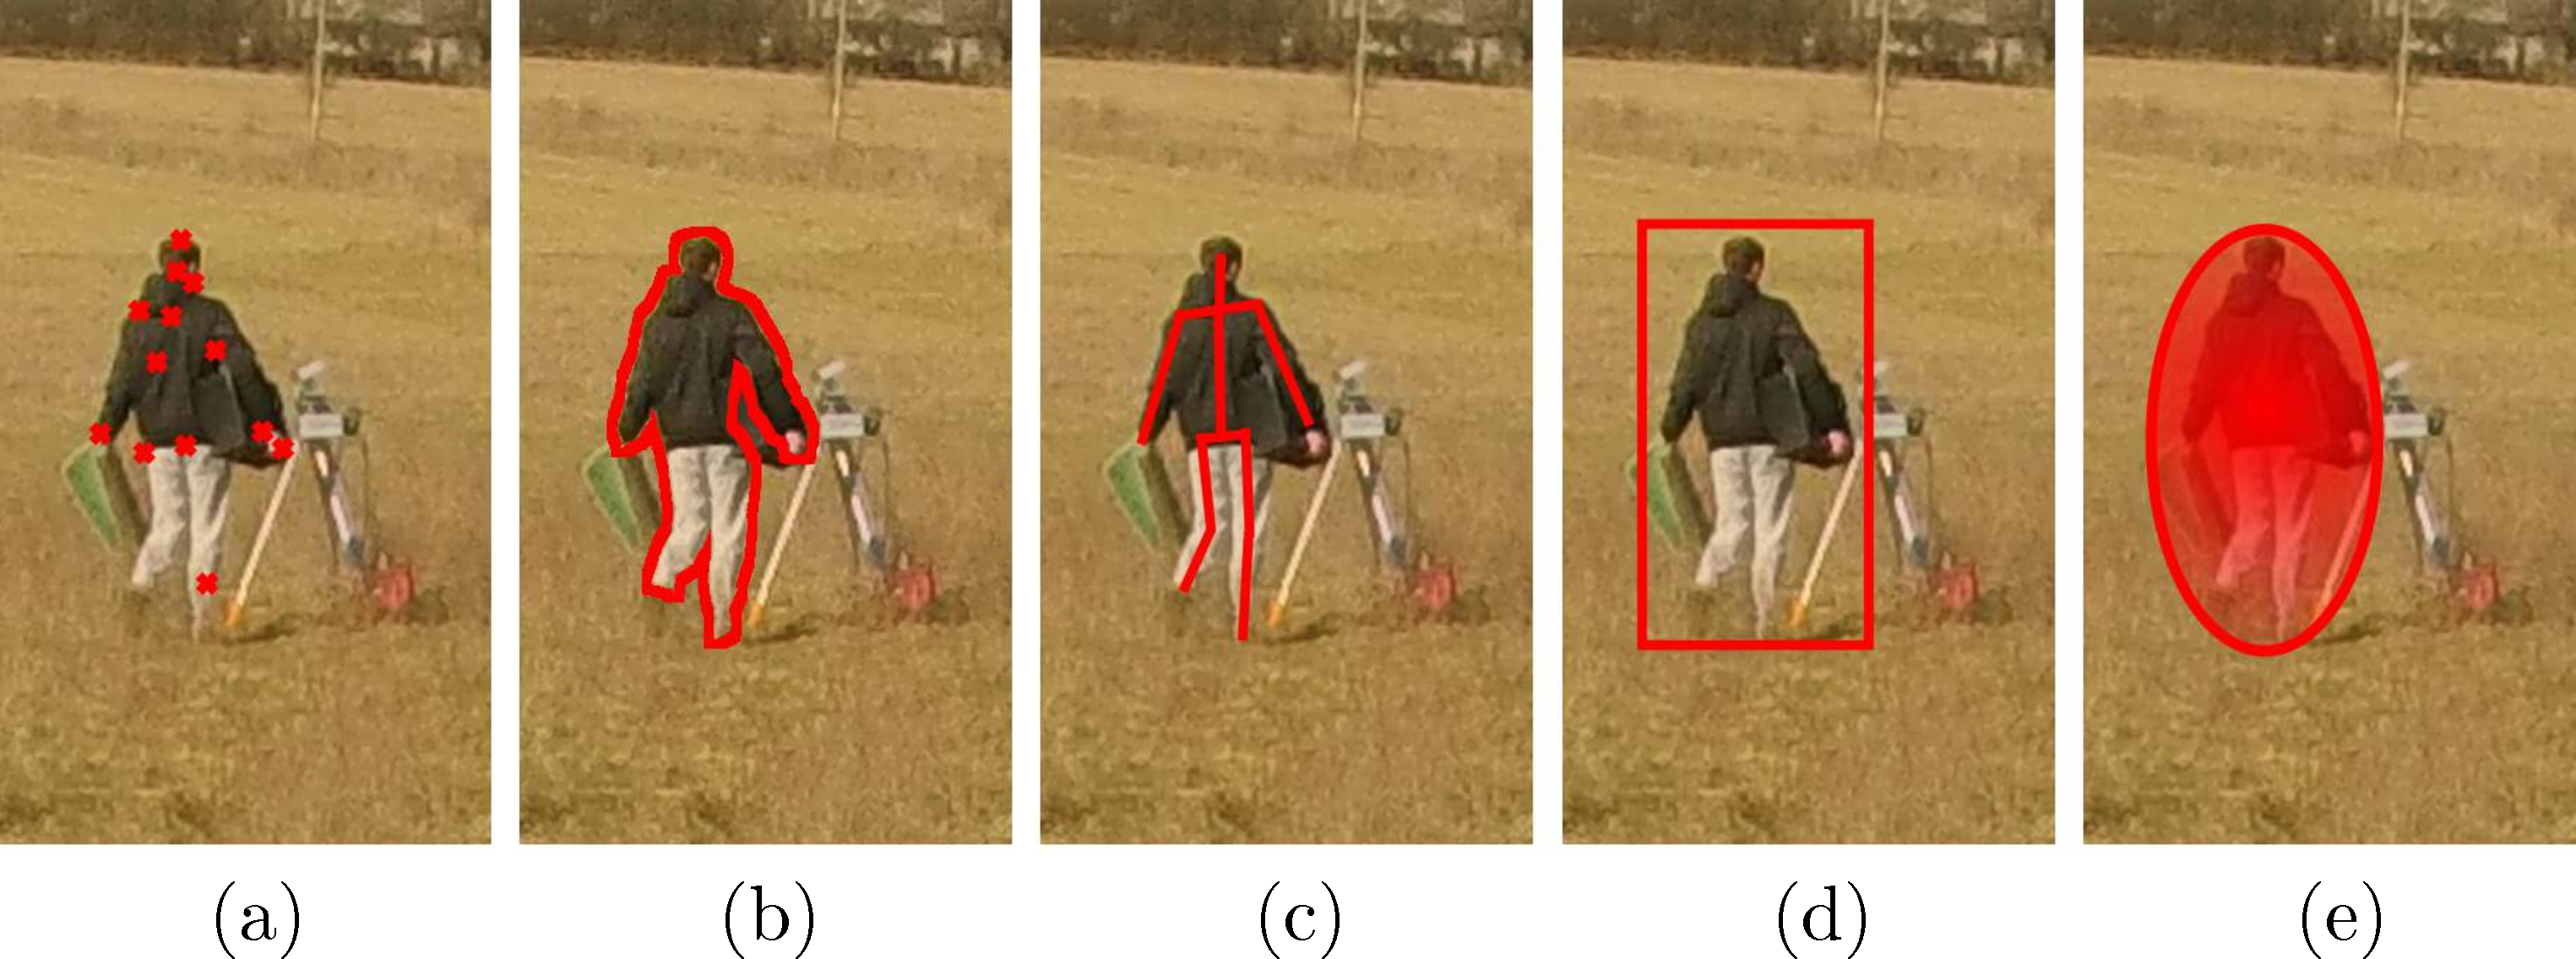
\includegraphics[width=0.7\textwidth]{fig/object_model.pdf}
	\caption{Various approaches to tracked object modeling. (a) Keypoints, (b) contour and (c) articulated model fall into the \textit{shape representation} category whereas (d) template and (e) kernel belong to the \textit{appearance representation} category. The intensity of a red color in case (e) denotes the weight of the given pixel in the given (ellipse shaped) kernel.}
	\label{fig:object_models}
\end{figure}

%.........................................................................
%.........................................................................
\subsection{Tracking approaches}

The main purpose of the tracker is to iteratively estimate the trajectory of the tracked object from frame to frame. There is a wide range of approaches to visual tracking and since they usually combine multiple various methods in order to reinforce the tracker robustness they cannot be really divided into distinct categories in a straightforward manner. However, the approaches can be coarsely categorized by the selection of the object representation.

To reinforce the tracker robustness the motion models are often used. Kalman filter and particle filter are the most popular ones \cite{cuevas2005kalman, ObjectTrackinginMonochromaticVideo}.


\subsubsection*{Keypoint Tracking} 
Keypoint tracking represents one of the most common approaches \cite{Tomasi91detectionand,Nebehay2014WACV}. The \textit{keypoint} is understood to be a single point in a an image which represents a small image region -- a \textit{point descriptor} -- and which should be highly discriminative and invariant to various image transformations. There are many widely used keypoint detectors/descriptors e.g. SIFT, SURF, ORB, FREAK, etc. \cite{sift, Bay:2008:SRF:1370312.1370556, Rublee:2011:OEA:2355573.2356268, Ortiz:2012:FFR:2354409.2354903} and they differ mainly in the means of matching precision and computation speed \cite{Schaeffer_acomparison, conf/icpr/MiksikM12}. What the tracker does is that it detects the keypoints and their descriptors in each frame, selects those representing the object, finds the correspondences and computes the transformation from the previous frame. Even though the keypoint tracking is well established approach it cannot be used in the OLS due to the insufficient size of the tracked objects as was explained in Section \ref{txt:object_model}.

\subsubsection*{Kernel Tracking}
Kernel approaches are based on so-called \textit{kernel}. Basically, the feature target representation is spatially masked with an isotropic kernel (for illustration see Figure \ref{fig:object_models} (e)) which assigns the largest weights to the pixels in the middle while the weights decay in the directions towards the edges of the kernel. This enables a spatially-smooth similarity function to be defined. Consequently, this function can be optimized in the means of target position using traditional gradient based methods such as gradient descent \cite{Comaniciu:2003:KOT:776753.776799}. To boost the robustness of the tracker multiple collaborative kernels might be used \cite{MultipleCollaborativeKernelTracking, Multi-kernelCorrelationFilterForVisualTracking}. The strategy to distinguish which pixels in the kernel/template are more or less reliable is also utilized in the BGFG tracker which the OLS is based on (see Section \ref{txt:bgfg_tracker}).

\subsubsection*{Tracking-by-Detection}
This class of approaches heavily utilizes the detection principles in combination with motion based approaches to localize the object \cite{eth_biwi_00633, Kalal:2012:TRA:2225045.2225082}. Depending on the object model the detection might be performed either by detecting keypoints and matching them against the pretrained model \cite{FastKeypointRecognitionInTenLinesOfCode, DBLP:journals/corr/abs-1211-5829} or by dividing the image into individual patches in which the object is searched for. For each patch the template matching is performed \cite{AFastTemplateMatchingAlgorithm, ObjectTrackinginMonochromaticVideo} (using SSD\footnote{Sum of Squared Differences.}, SAD\footnote{Sum of Absolute Differences.} or NCC\footnote{Normalized Cross Correlation.} as a similarity measure) or feature set is extracted; consequently, the model presence probability is evaluated using the generative or the discriminative classifier \cite{EnhancedGaussianMixtureModels, EfficientScan-windowGPGPU}. Since the exhaustive search within the whole image is computationally expensive, the cascade classifiers might be applied \cite{violaJones, RobustObjectDetectionViaSoftCascade}. The TLD approach which is used in the OLS utilizes the object detector in order to correct and/or reinitialize the tracker (see Section \ref{txt:tracking_learning_detection}).

\subsubsection*{Motion Based Tracking}
This category of approaches attempts to extract the motion occurring between the consecutive images. The \textit{optical flow} method which in general tries to find the motion of individual pixels in the image can be used to track the keypoints \cite{Bouguet00pyramidalimplementation} or to produce the binary feature images and consequently the blobs corresponding to moving objects \cite{aslani2013optical}. Alternatively, the moving object can be detected in the image regions yielding the highest response of \textit{frame differencing} (known also as \textit{background subtraction}) \cite{Noh2013, Movingobjectdetection}. The BGFG tracker which the OLS uses is based on the frame differencing to estimate the appearance model and most likely location of the tracked object (see Section \ref{txt:bgfg_tracker}).

\subsubsection*{Motion Modeling}
The tracking can be approached through the model of a discrete-time dynamic system, where the aim is to estimate the current state for each incoming frame \cite{Comaniciu:2003:KOT:776753.776799}. The state can be represented as a mere 2D position of a target (in pixel-coordinates) or other parameters such as velocity or acceleration of a target can be modeled a well. Thanks to the motion model the (computationally expensive) exhaustive search for the object can be reduced to the vicinity of the current target position estimate.

\paragraph{Kalman filter} 
Kalman filtering is one of the widely used technique for recursively evaluating the current state of a target given the measurement corrupted by the measurement noise and the prediction of the next state corrupted by the process noise \cite{Welch:1995:IKF:897831, cuevas2005kalman}. It is based on the assumption that the state posterior density is Gaussian and thus can be parametrized by means and covariances. However, this assumption might not hold. In case of the OLS a camera used for tracking is often in motion and the sensory data about its position which could be used to stabilize the motion might be imprecise or not available at all (for illustration see Figure \ref{fig:kalman}). Consequently, the position of a tracked object can change rapidly from frame to frame and thus to defy the assumption of the Gaussian distribution of the state posterior density. Furthermore the basic Kalman filter is based on unimodal Gaussian distribution which prevents it from keeping multiple hypothesis for a single target.

%% Kalman filter illustration
\begin{figure}[tbh]
	\centering
	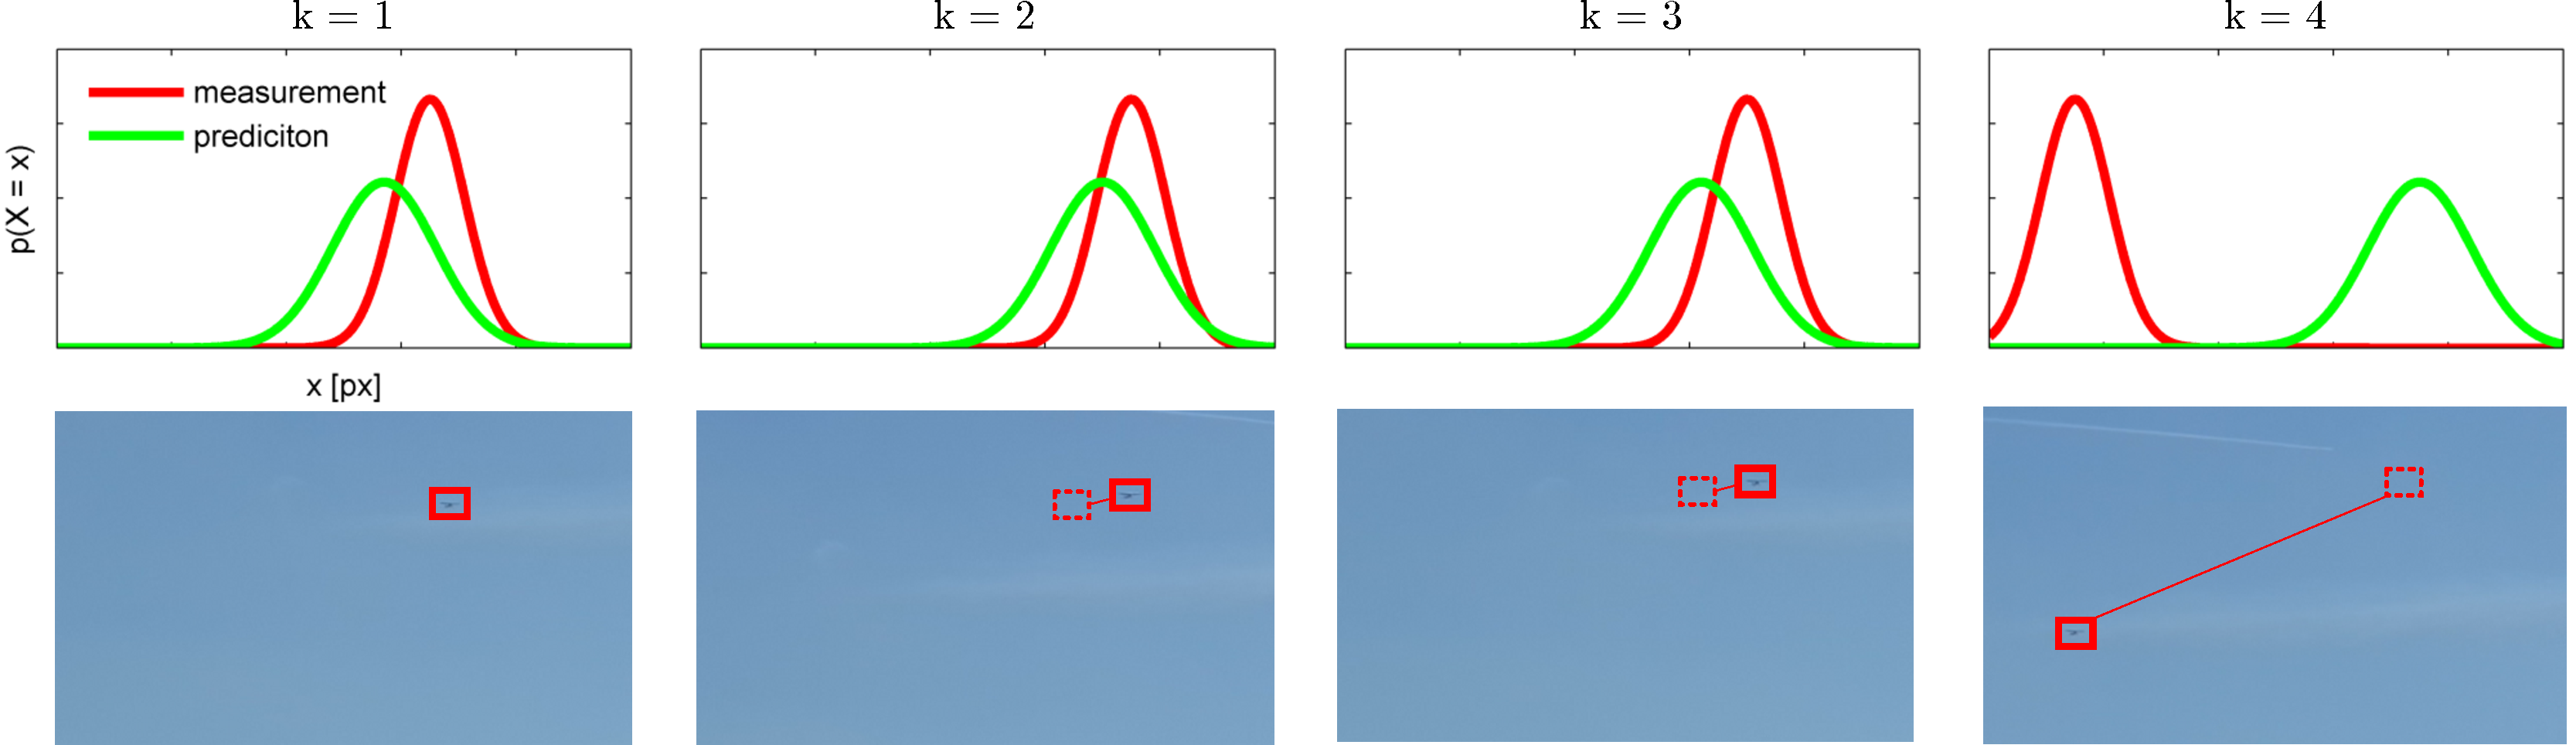
\includegraphics[width=0.95\textwidth]{fig/kalman.pdf}
	\caption{The evolution of measurement and prediction probability density of the tracked target in the Kalman filter framework. The target apparently moves along a line with constant velocity, however, in frame $k = 4$ it suddenly changes its position due to the rapid camera movement which is something that Kalman filter cannot cope with.}
	\label{fig:kalman}
\end{figure}

\paragraph{particle filter} 
The particle filter represents the most general class of filters which can cope with non-Gaussian state and measurement processes as well as with tracking multiple hypothesis \cite{journals/cviu/BimboD11}. Current state of the system is represented as a \textit{particle} $\particle{t}{i}$ -- a vector of parameters ${\vec{x_{t}^{i}}}$ describing the properties of tracked object (e.g. position, velocity, acceleration, etc.) and assigned scalar weight $w_{t}^{i}$. The suitable \textit{fitness function} must be proposed to evaluate how well a particle fits to the observed data. Using finite number of particles the particle filter basically samples the fitness function (which might be arbitrarily complex and non-differentiable) in an attempt to find the optimum. A bootstrap particle filter (BPF) is a variant of particle filter widely used for visual tracking \cite{Isard98condensation}. It follows the sequential importance sampling principle -- in each iteration the particles with higher weights are duplicated while the particles with lower weights are discarded \cite{doucet2001sequential}. This enables higher resolution sampling of the fitness function only in the parts which are likely to contain the (local) optimum. The BPF iteratively performs four main steps -- \textit{resampling}, \textit{prediction}, \textit{update} and \textit{weights normalization}. The detailed breakdown of all steps is depicted in Algorithm \ref{alg:bpf}. Note that the function $predict()$ in \textit{update} step should correspond to the required motion model of the tracked object (a normal distribution $\mathcal{N}(\mu, \sigma)$ is given as an example) and it can be designed to allow for the rapid camera motion which suits the needs of the OLS. Therefore, the tracker based on BPF is utilized (see Section \ref{txt:bgfg_tracker}).

\begin{algorithm}
	\SetAlgoNoLine	
	\KwIn{A measurements $M$, a set of particles $P = \{\particle{t}{1}, \particle{t}{2}, ..., \particle{t}{n_{p}}\}$}
	\KwOut{The particle $\particle{t}{i_{bestParticle}}$ representing the state estimation with best weight $w_{t}^{i}$}
	\DontPrintSemicolon
	\SetCommentSty{textsc}
	
	\BlankLine
	
	\tcc{Resampling (importance sampling)}
	$resampleParticles()$\;
	
	\BlankLine
	\tcc{Prediction}
	\ForEach{$\particle{t}{i} \in P$}
	{
		\ForEach{parameter $k_{j}$ of ${x_{t}^{i}}$}
		{		
			$predict(k_{j})$ /* (e.g. $k_{j} = k_{j} + x, ~ x \sim \mathcal{N}(\mu_{j}, \sigma_{j})$) */ \;
		}
	}
	
	\BlankLine
	\tcc{Update}
	\ForEach{$\particle{t}{i} \in P$}
	{
		$w_{t}^{i} = fitnessFunction(M, \particle{t}{i})$\;
	}
	
	\BlankLine
	\tcc{Estimate final state e.g. using MAP}
	$\particle{t}{i_{bestParticle}} = \particle{t}{i} \in P : !\exists ~ \particle{t}{j} \in P : w_{t}^{j} > w_{t}^{i}$\;
	
	\BlankLine	
	\tcc{Weights normalization}
	\ForEach{$\particle{t}{i} \in P$}
	{
		$w_{t}^{i} = \frac{w_{t}^{i}}{\sum_{j = 1}^{n_{p}}w_{t}^{j}}$
	}
	
	
	\caption{Tracking using BPF}
	\label{alg:bpf}
\end{algorithm}

%.........................................................................
%.........................................................................
\subsection{Tracking-Learning-Detection} \label{txt:tracking_learning_detection}

The Tracking Learning Detection (TLD) \cite{Kalal:2012:TRA:2225045.2225082} is an algorithm designed for performing so called long-term tracking -- a robust tracking of an object which might change its appearance, be temporarily occluded by closer objects or temporarily completely disappear from the scene. TLD is based on the appearance representation of the target, specifically a set of templates is stored and continuously updated. Additionally, TLD can be implemented to run in real-time. Such properties meet the requirements of the OLS (see Section \ref{txt:introduction}), thus TLD is incorporated in OLS as one of the visual trackers and this section explains its design in more detail.

Since a long-term tracking cannot be easily achieved either by a mere tracker nor by a detector, the TLD aims to combine the strengths of the detection and tracking algorithms by combining their results. Furthermore, the algorithm incorporates the online adaptation subsystem capable of learning the new appearances of the tracked object over the course of the tracking.

A conceptual diagram of the TLD algorithm is shown in Figure \ref{fig:tld_block_diagram}. The \textit{tracking} component tracks the object and for each frame produces the new position. It expects that object does not disappear (occlusion, out of FOV) from the scene and if it does, the tracker fails. The \textit{detection} component performs full scanning of the image for each frame. It detects the object and if needed it reinitializes the tracker. The \textit{learning} component is capable of generating new appearances of the tracked object and thus improving the performance of the detector. 

The object itself is modeled as a set of patches, each patch being already learned appearance represented by the rectangular bounding box around the object rescaled to a normalized resolution of 15 x 15 pixels. The similarity of the patches is given by NCC.

%% TLD block diagram
%% TLD PN learning block diagram
\begin{figure}[htb]
	\centering
	\begin{minipage}{.34\textwidth}
		\centering
		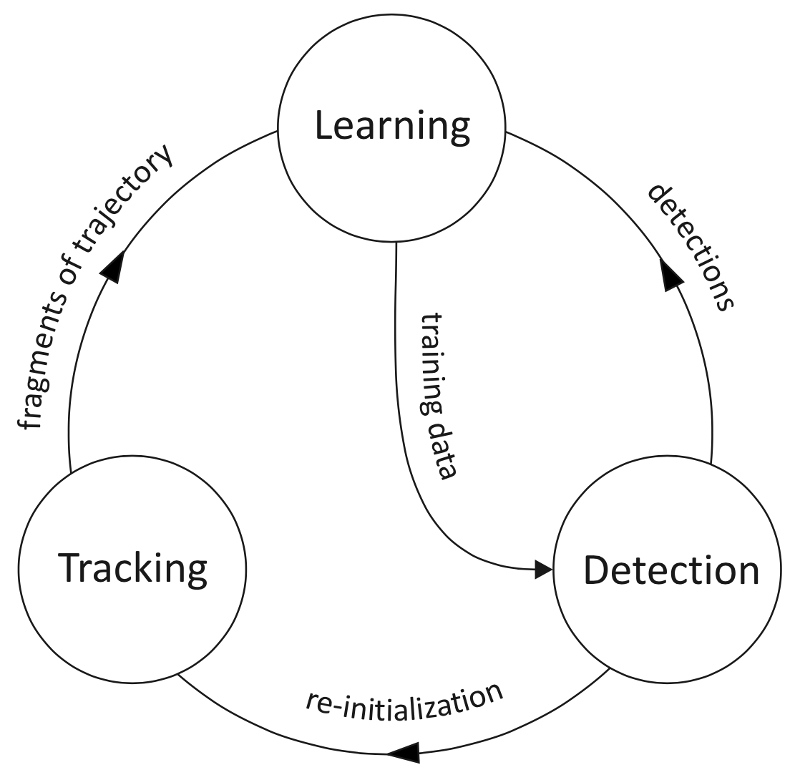
\includegraphics[width=.99\linewidth]{fig/tld_block_diagram.png}
		\captionof{figure}{A diagram of the main TLD components. Image is adopted from authors Kalal, Mikolajczyk and Matas \cite{Kalal:2012:TRA:2225045.2225082}.}
		\label{fig:tld_block_diagram}
	\end{minipage}
	\hfill
	\begin{minipage}{.63\textwidth}
		\centering
		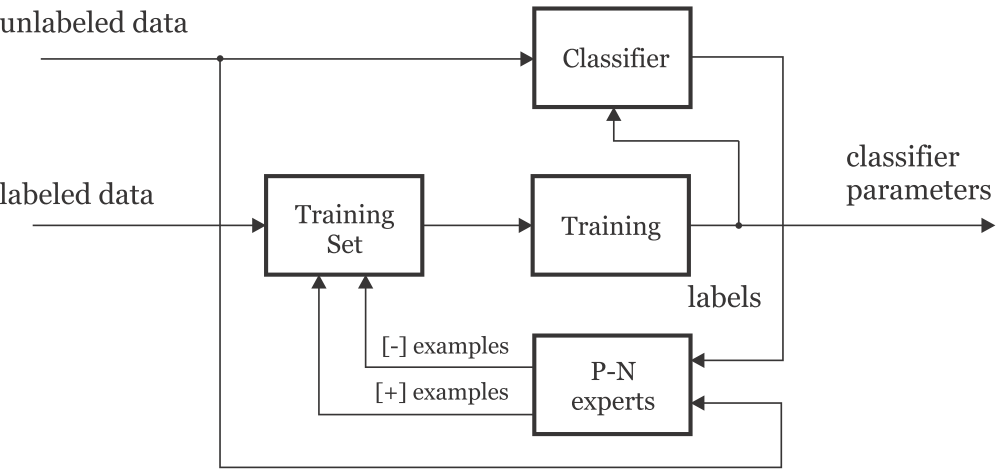
\includegraphics[width=.99\linewidth]{fig/tld_pn_learning_block_diagram.png}
		\captionof{figure}{A diagram of the PN learning process. Image is adopted from authors Kalal, Mikolajczyk and Matas \cite{Kalal:2012:TRA:2225045.2225082}.}
		\label{fig:tld_pn_learning_block_diagram}
	\end{minipage}
\end{figure}

\paragraph{Detection} The detector treats each frame as an independent one and scans a full image. A scanning window is used and it is gradually scaled (in order for the detector to achieve scale invariance) and iteratively shifted along a regular grid of candidate positions. Since this task is computationally intensive a cascade classifier is used so that the detector could quickly decide whether a given subregion contains the object. In case of TLD the cascade classifier consists of three sequential stages specifically ordered so that earlier the stage is the more subregions it should reduce while being computationally less expensive. Should the subregion be rejected by any stage later stages ignore it completely.

\paragraph{Tracking} The tracking subsystem is based on the algorithm called the Median-Flow tracker. A $10 \times 10$ grid is used to select the positions within the bounding box representing the object. For each position a given point is tracked between the consecutive frames using pyramidal Lucas-Kanade tracker and eventually the tracker only accepts a 50~\% of the most reliable displacements to estimate a new position of the target.

\paragraph{Learning} Since the classifier used in the detection phase is initially trained using only one positive patch (the initial bounding box selected by user) it tends to make errors as a video stream progresses since the moving object of interest changes its appearance due to the transformation caused by its motion. Therefore, online component called \textit{P-N learning} is incorporated in the system and it gradually extends the training sets. Two experts are used. \textit{P-expert} identifies only false negatives while \textit{N-expert} identifies only false positives. Once a wrongly classified patch is found the experts extend the training set and the classifier is retrained (see Figure \ref{fig:tld_pn_learning_block_diagram}).

%.........................................................................
%.........................................................................
\subsection{Tracking Using Background/Foreground Modeling and Particle Filter} \label{txt:bgfg_tracker}

The autonomous tracking uses the implementation of the visual tracker combining the background subtraction, motion model and object model in the particle filter framework  proposed in \cite{ObjectTrackinginMonochromaticVideo} (BGFG tracker). Thanks to both particle filter and inter frames homography computation this approach can even cope with the moving cameras. Partial occlusion is handled using foreground modeling and the tracker is capable of running in real-time. Therefore, this approach is suitable for the OLS as well and it is used as an alternative to TLD. The operation of the tracker is described below.

The target is represented as a rectangular template (consisting of gray-scale intensity values) which is normalized to the size $24\times24$ pixels. The template is created only once during the initialization, thus the tracker could fail if the target changed its appearance significantly during the course of tracking. However, in case of very distant targets only a slight change occurs.

The Bootstrap particle filter (BPF) \cite{Isard98condensation} is used to generate and evaluate candidate positions of the target. Each particle (i.e. the state of the system) is represented as $\vec{x_{n}} = (x, y, v_{x}, v_{y}, h, w)$, where $(x, y)$ represents the 2D position of the target, $(v_{x}, v_{y})$ represents the estimated speed of the target and $(h, w)$ represents the bounding box size. 

The perturbations in the observed position of the target caused by the moving camera are alleviated using the motion model which is applied in the \textit{prediction} step of the BPF:
\begin{align}
	pos_{n+1} &= pos_{n} + vel_{n} + \gamma_{pos} \sim \mathcal{N}(\mu, \sigma),\\ \label{eq:bgfg_pos_prediction}
	vel_{n+1} &= vel_{n} + \gamma_{vel} \sim \mathcal{N}(\mu, \sigma),\\
	bb_{n+1} &= bb_{n} + \gamma_{bb} \sim \mathcal{N}(\mu, \sigma),	
\end{align}
where scalar $pos_{n}$ is the $x$ or $y$ position, scalar $vel_{n}$ is the $x$ or $y$ velocity, scalar $bb_{n}$ is the $w$ or $h$ size of the bounding box in time $n$, and $\gamma$ is the noise drawn from the Gaussian distribution $\mathcal{N}(\mu, \sigma)$, where scalars $\mu$ and $\sigma$ parameters are set empirically for each parameter.

In the \textit{update} step, each particle is assigned a new weight $w$ using the objective function reflecting the similarity of the template and the candidate patch, The function serves the purpose of the similarity measure and it is based on a SSD:
\begin{align} \label{eq:bgfg_distance_function}
	w = \sum_{(x,y) \in I}{e^{min(M_{t}^{(x,y)}, M_{c}^{(x,y)})}(1 - |I_{t}^{(x,y)} - I_{c}^{(x,y)}|)^{2}},
\end{align}
where $M_{t}$ and $M_{c}$ are the foreground masks (FM) of the template and the current candidate respectively, $I$ is the image, $t, c$ subscripts denote template and candidate patch respectively, and $(x,y)$ superscript denotes indexing 2D array (an image). The FMs are estimated by subtraction of the two images where the bounding boxes denoting the position of the target do not overlap (the FM $M_{t}$ is estimated only once). The resulting estimate of the target position is chosen using the Maximum a posteriori approach.

In order to enable the motion of the camera the transformation between each pair of adjacent frames is estimated by detecting and tracking the keypoints using KLT tracker \cite{Tomasi91detectionand} and then estimating the homography using the RANSAC algorithm \cite{Hartley:2003:MVG:861369}.

%\section{Motion Prediction and Regulation}
%
%%.........................................................................
%%.........................................................................
%\subsection{2D and 3D Position Prediction}
%\todo{moving average}
%\todo{linearni regrese}
%\todo{RANSAC}
%
%%.........................................................................
%%.........................................................................
%\subsection{Hardware Regulation}
%\todo{PID}
%\todo{funkcni zavislost rychlosti na vzdalenosti cile od stredu}

%-------------------------------------------------------------------------
%-------------------------------------------------------------------------
\section{Multi-camera Target Localization} \label{txt:multi_camera_target_localization}

This section introduces the problematics of estimating the location of a target in 3-space given the arbitrary number of corresponding image points in 2-space. First, the suitable camera model is described, then the standard stereo setups are examined, next the notion of triangulation with noisy measurements is presented and finally the existing approaches to target location estimation as well as their suitability for OLS are discussed.

\subsection{Camera Model}

Localization of a target corresponds to a process of mapping image locations of a target in 2-space from multiple cameras to a location in 3-space. Thus it is necessary to define a model of a camera first. The \textit{finite pinhole camera} based on the \textit{central projection} is a standard approach to model cameras with CCD like sensors \cite{Hartley:2003:MVG:861369} and it is used to model hardware cameras in OLS as well. Finite pinhole cameras use projection matrix $P$ which maps a point $\vec{X}$ in 3-space to an image location $\vec{x}$ in 2-space (see Figure \ref{fig:pinhole_camera}):

\begin{align}
	\vec{x} &= P\vec{X},\\
	P &= KR[I|-C],\\
\end{align}
where $I$ is the identity matrix, $R$ and $C$ are the rotation and translation matrices representing the orientation and position of the camera frame with respect to the world frame and $K$ is the \textit{intrinsics matrix} (or \textit{camera calibration matrix}) consisting of a focal length $f$, coordinates of the principal point $PP = (x_{0}, y_{0})^{T}$ and skew parameter $s$:
\begin{align}
	K = \begin{bmatrix}
		\alpha_{x} & s          & x_{0} \\
		0          & \alpha_{y} & y_{0} \\
		0          & 0			& 1
	\end{bmatrix}.
\end{align}

%% Pinhole camera
\begin{figure}[tbh]
	\centering
	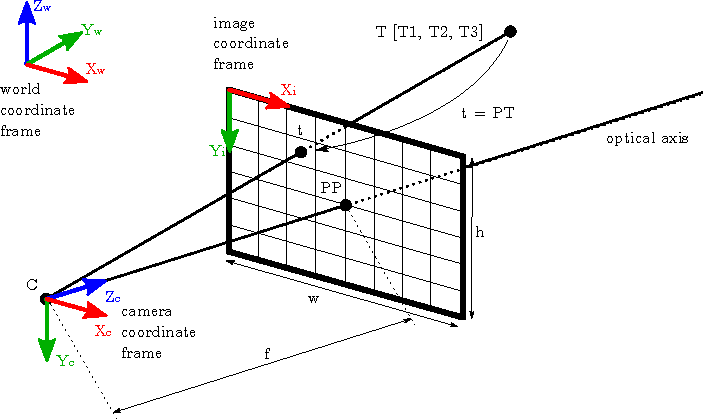
\includegraphics[width=0.60\textwidth]{fig/pinhole_camera.pdf}
	\caption{Perspective projection of pthe oint $T$ in 3-space to the point $t$ in 2-space located on the image plane in the finite pinhole camera model.}
	\label{fig:pinhole_camera}
\end{figure}

\subsection{Stereo Setups}

With two calibrated cameras (i.e. $K$, $R$ and $C$ matrices are known) observing the same portion of the environment it is possible to estimate the location of the given point/object in 3-space. The \textit{canonical stereoscopic system} is one of the widely used setup capable of estimating the depth of points in the scene \cite{Cyganek:2007:ICV:1214366}. The optical axes of both cameras are collinear and the notion of \textit{disparity} is introduced. Disparity refers to the difference in the image location of the same 3D point when projected under perspective to two different cameras \cite{Stockman:2001:CV:558008} and the coordinates of a point in 3-space can derived using following equations (see Figure \ref{fig:canonical_vs_general_stereo}):

\begin{align}
	z &= fb/(x_{l} - x_{r}) = fb/d,\\
	x &= x_{l}z/f = b + x_{r}z/f,\\
	y &= y_{l}z/f = y_{r}z/f,
\end{align}
where $f$ is the focal length, $b$ is the baseline, $x_{l}$ and $x_{r}$ are the horizontal distances between the principal points $PP$ of the respective camera and the projection $t_{l}$ and $t_{r}$ respectively (the same applies for $y_{l}$ and $y_{r}$ in vertical direction), $d$ is the disparity and $(x, y, z)^{T}$ are the 3-space coordinates of the target. Nevertheless, the OLS cannot be modeled as canonical stereoscopic system due to the fact that it is designed to work with arbitrary number of cameras and furthermore, the extrinsics of the cameras are not fixed (the cameras rotate freely in space, see Section \ref{txt:design_of_the_OLS}).

%% Canonical stereo setup vs general stereo setup
\begin{figure}[tbh]
	\centering
	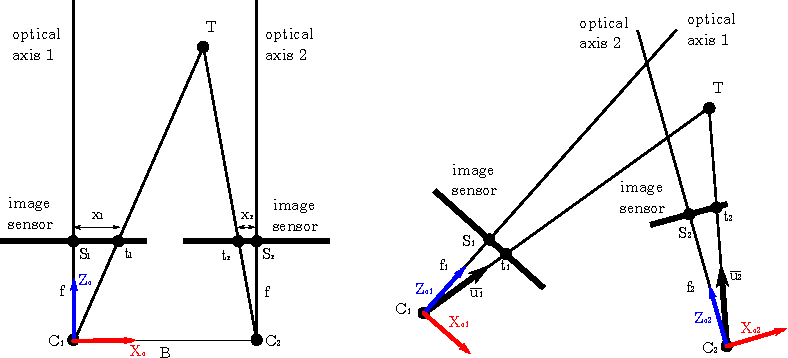
\includegraphics[width=0.8\textwidth]{fig/canonical_stereo_vs_general_stereo.pdf}
	\caption{In canonical stereo setup (left) the 3D coordinates of the given point can be computed using the notion of disparity. On the other hand, in case of general stereo setup (right) the intersection of lines in 3-space defined by the target projected to the image space of each camera must be found.}
	\label{fig:canonical_vs_general_stereo}
\end{figure}

In \textit{general stereo setup} the collinearity of the optical axes is not required. However, location of a point in 3-space cannot be simply estimated through triangle similarity. On each camera a line in 3-space mapping to a point $\vec{p_{i}}$ in 2-space has to be first computed using \textit{back-projection} (see Figure \ref{fig:canonical_vs_general_stereo}):
\begin{align}
	X(\lambda) = P^{+}\vec{x} + \lambda C,
\end{align}
where $P^{+}$ is the pseudo-inverse of $P$ ($P^{+} = P^{T}(PP^{T})^{-1}$). The location of the target in 3-space is then given as an intersection of all back-projected lines. Given its nature the OLS can be modeled as a general stereo setup extended to use arbitrary number of cameras (instead of only two cameras).

\subsection{Triangulation with Noisy Measurements} \label{txt:triangulation_with_noisy_measurements}

The process of finding the location of a target in 3-space as an intersection of back-projected lines is called \textit{triangulation}. In ideal case the projection matrices $P_{i}$ and calibration parameters are known precisely for both cameras and the lines in 3-space intersect. However, in real world the system is subject to both systematic and random error (see Chapter \ref{txt:precision_of_the_localization}), consequently the lines in 3-space might become skew (i.e. they are not guaranteed to intersect anymore) since the stereo system does not satisfy the epipolar constraint \cite{Hartley:2003:MVG:861369} (more detailed explanation can be found in Section \ref{txt:3d_environment_reconstruction}):
\begin{align}
	\vec{x'}^{T}F\vec{x} \neq 0.
\end{align}

In general, the same problem holds within each pair of cameras in N-view setup. Instead of the intersection the minimum distance between each pair of skew lines might be found as a line segment perpendicular to both skew lines (see Figure \ref{fig:multi_view_intersection}) via following equation \cite{Forsyth:2002:CVM:580035}:
\begin{align}
	z_{ij}\vec{p_{i}} &= \vec{T_{ij}} + z_{ij}R_{ij}\vec{p_{j}} + \lambda_{ij}(\vec{p_{i}} \times R_{ij}\vec{p_{j}})\\
	for~i,j           &= 1,2,...,N \land i \neq j,
\end{align}
where $\vec{p_{i}}$ is the direction of back-projected line in camera $i$, $z_{ij}$ gives the scale of vector ${p_{i}}$ so as to define a point $P_{ij}$ which is the closest to the line back-projected from camera $j$, $T_{ij}$ and $R_{ij}$ are the translation and rotation of the coordinate frame of the camera $j$ with respect to the coordinate frame of the camera $i$ and $\lambda_{ij}$ defines the length of the line segment connecting both back-projected skew lines.

A similar approach to finding the closest distance between each pair of cameras is used in the OLS (see Section \ref{txt:target_localization_using_triangulation}).

%% Skew lines in multi view scenario
\begin{figure}[tbh]
	\centering
	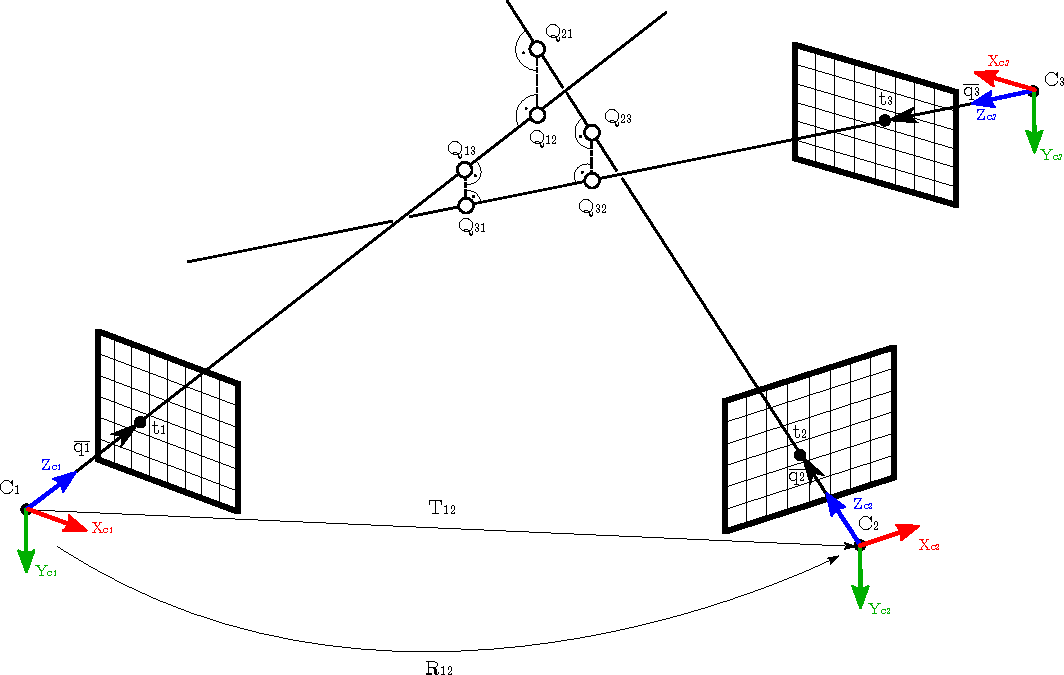
\includegraphics[width=0.9\textwidth]{fig/multi_view_intersection.pdf}
	\caption{An example of a three-view setup and the target location estimation using triangulation. Since all cameras are subject to systematic and random error the back-projected lines are skew, thus there is no intersection. The closest distance between each pair of lines is given by the line segment perpendicular to both lines.}
	\label{fig:multi_view_intersection}
\end{figure}

\subsection{Estimation of Target Location} \label{txt:estimation_of_target_location}

Since the back-projected lines are skew, there is not the only correct solution to the localization problem. Contrarily, the position of the target must be estimated. Hartley and Zisserman \cite{Hartley:2003:MVG:861369} propose a couple of methods where the approaches basically boil down either to solving the overdetermined system of linear equations or to minimization of the geometric error. Both approaches are briefly described below.

\paragraph{Direct Linear Transformation (DLT)} The DLT algorithm is based on the assumption that an overdetermined system of linear equations in the form $\matr{A}\vec{x} = \vec{0}$ (where $\matr{A}$ is the matrix of coefficients, $\vec{x}$ is the vector of unknowns and $\vec{0}$ is the zero vector) is available and that given the noise there is no exact solution. In case of a stereo setup where the image points $\vec{t_{1}}$ and $\vec{t_{2}}$ in 2-space on each camera correspond to a target $\vec{T}$ in 3-space the overdetermined system of linear equations can be defined with vector $\vec{x} = (t_{1}^{x}, t_{1}^{y}, t_{2}^{x}, t_{2}^{y})$ and matrix $\matr{A}$:
\begin{align}
	A = \begin{bmatrix}
		t_{1}^{x}\vec{p_{1}^{3}}^{T} - \vec{p_{1}^{1}}^{T} \\
		t_{1}^{y}\vec{p_{1}^{3}}^{T} - \vec{p_{1}^{2}}^{T} \\
		t_{2}^{x}\vec{p_{2}^{3}}^{T} - \vec{p_{2}^{1}}^{T} \\
		t_{2}^{y}\vec{p_{2}^{3}}^{T} - \vec{p_{2}^{2}}^{T} \\
	\end{bmatrix},
\end{align}
where $\vec{p_{cam}^{r}}$ is the $rth$ row of the projection matrix $\matr{P_{cam}}$ of the camera $cam$. The ultimate solution is found using the SVD\footnote{Singular Value Decomposition} as the singular vector corresponding to the smallest singular value of $\matr{A}$.

\paragraph{Reprojection Error Minimization} Similarly as DLT this method assumes that the correspondence between image points $\vec{t_{1}}$ and $\vec{t_{2}}$ does not meet the epipolar constraint. The aim thus is to estimate the position of the target $\vec{T}$ in 3-space which projects to image points $\vec{t_{1}'}$ and $\vec{t_{2}'}$ satisfying the epipolar constraint and which at the same time minimizes the reprojection error function $ref$:
\begin{align}
	ref(\vec{t_{1}}, \vec{t_{2}}) = d(\vec{t_{1}}, \vec{t_{1}'})^{2} + d(\vec{t_{2}}, \vec{t_{2}'})^{2},
\end{align}
where $d(\vec{x}, \vec{x'})$ is the Euclidean distance between the measurement $\vec{x}$ and reprojected image point $\vec{x'}$ (see Figure \ref{fig:reprojection}). The reprojection error function can be either minimized using any optimization method or the minimum can even be found non-iteratively in closed form.

%% Reprojection
\begin{figure}[tbh]
	\centering
	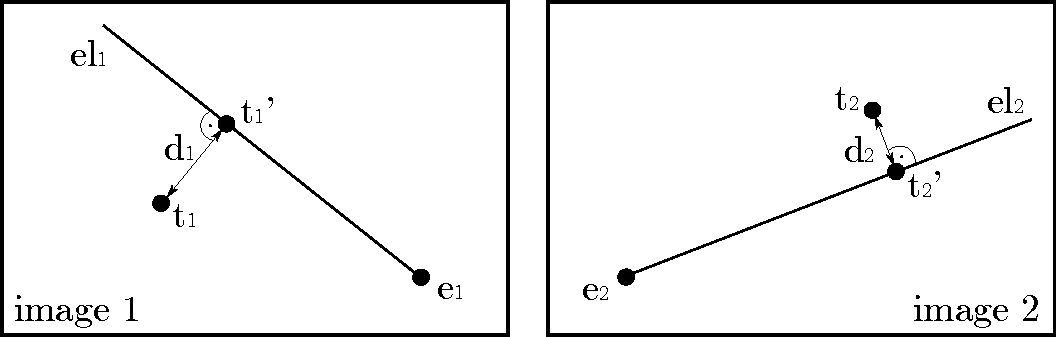
\includegraphics[width=0.6\textwidth]{fig/reprojection.pdf}
	\caption{The demonstration of reprojection error in a stereo setup where $e_{i}$ is the epipole, $el_{i}$ is current estimation of epipolar line and $d_{i}$ is the Euclidean distance between the initial noisy measurement $t_{i}$ and the reprojection of the target estimate $t_{i}'$ in the camera $i$.}
	\label{fig:reprojection}
\end{figure}

Even though both DLT and reprojection error minimization could be extended so as to support multiple-view setup, neither of these approaches is suitable for the OLS since they do not consider any a priori known information about the reliability of the back-projected line in each camera. It has been shown that in the OLS the precision of target location estimation strongly depends on the mutual position of the target and the baseline of the given camera pair (see Chapter \ref{txt:precision_of_the_localization}). Furthermore, it is possible to obtain the belief from individual visual trackers (i.e. the confidence that the object is tracked correctly). In order to exploit these prior information a specific location estimation method was proposed for the OLS (see Section~\ref{txt:target_localization_using_triangulation}).

%\subsection{Existing Multi-Camera Localization Systems}
%
%Professional systems aiming on automatic localization of aerial (as well as terrestrial and underwater) targets mostly rely on active devices, such as radars or sonars and there is very little use of pure passive optical devices (such as RGB cameras, thermal imaging cameras, etc.). The reason might be the complexity of the whole solution or the operation constrained by the weather conditions.
%
%On the other hand since the application of multiple view geometry has been one of hot topics in the computer vision during the past decade, many R\&D groups (specializing mostly on robotics) attempt to base their solutions on multi-camera optical localization.
%
%Professional systems aiming on automatic localization of aerial, terrestrial and/or underwater targets mostly rely on active devices, such as radars or sonars and there is very little use of pure passive optical devices (such as RGB cameras, thermal imaging cameras, etc.). As of today the multi-camera optical localization systems are mostly used for R\&D purposes and mainly in robotics. A common approaches is to set up so called \textit{intelligent space} \cite{intelligentSpace}, the bounded area under surveillance of multiple cameras reporting to the the central system. 
%
%In \cite{Multi-Camera_Sensor_System_for_3D_Segmentation} multiple terrestrial robots are detected, tracked and localized by the multi-camera system. For all cameras, the intrinsics and extrinsics are known beforehand and do not change over time.  A similar approach is used also in \cite{Localization_and_Geometric_Reconstruction_of_Mobile_Robots} but this system uses the robot's odometers as well in order to improve the resulting position estimated by the optical system. The system presented in \cite{A_3D_visual_localization} then relies on four ordinary RGB cameras with known parameters (intrinsics, extrinsics) to estimate the position of the easy to detect and static object using the Perpendicular Foot Method algorithm.
%
%Even though all of the aforementioned approaches utilize the ordinary RGB cameras for detection and tracking and in general estimate the location of the object using the triangulation algorithm, they all assume the object moves strictly within the specified bounded region and they rely on fixed positions of the cameras. Thus, they do not have to deal with the imprecisions arose from the uncertainty of the current camera pose estimation and with the problems of handing off the target to other camera units once a target moves out of the operational range of the given camera. 

%-------------------------------------------------------------------------
%-------------------------------------------------------------------------
\section{3D Environment Reconstruction} \label{txt:3d_environment_reconstruction}

One of the most challenging and still not fully solved problems of visual tracking algorithms is the occlusion \cite{Zhang:2010:RVT:1937728.1937766, conf/iccv/KwakNHH11}, i.e. the case where the tracked object becomes partially or fully overlapped by another object. Even though both visual trackers the OLS is based on (see Sections \ref{txt:tracking_learning_detection} and \ref{txt:bgfg_tracker}) are robust against partial occlusion and to the limited extent even against full occlusion, they detect the occlusion using the visual clues which might not be reliable. 

However, if the 3D model of the surrounding scene is known and motion model in 3-space of the tracked target is estimated, it is possible to predict both start and end of full occlusion occurrence in advance and consequently to adjust the tracking algorithm temporarily so that it would not fail. If the 3D model of the environment is not known beforehand it can be reconstructed using mere visual information obtained from cameras.

Therefore, this section introduces the problematics of 3D reconstruction using visual cues in multi-camera system, namely the basics of epipolar geometry, the notion of bundle adjustment and a popular tool for performing both sparse and dense reconstruction in multiple-camera setup -- VisualSFM. Proposed algorithm of occlusion prediction based on the knowledge of sparse 3D model of the environment is presented in Section \ref{txt:occlusion_prediction}. 

%.........................................................................
%.........................................................................
\subsection{Reconstruction Pipeline} \label{txt:reconstruction_pipeline}

Assuming the most general scenario where multiple images of the scene taken from multiple uncalibrated cameras are available, a 3D reconstruction pipeline based on the \textit{iterative bundle adjustment} can be utilized \cite{Snavely:2006:PTE:1179352.1141964} (see Figure \ref{fig:3d_reconstruction_pipeline}).

%% 3D reconstruction pipeline
\begin{figure}[tbh]
	\centering
	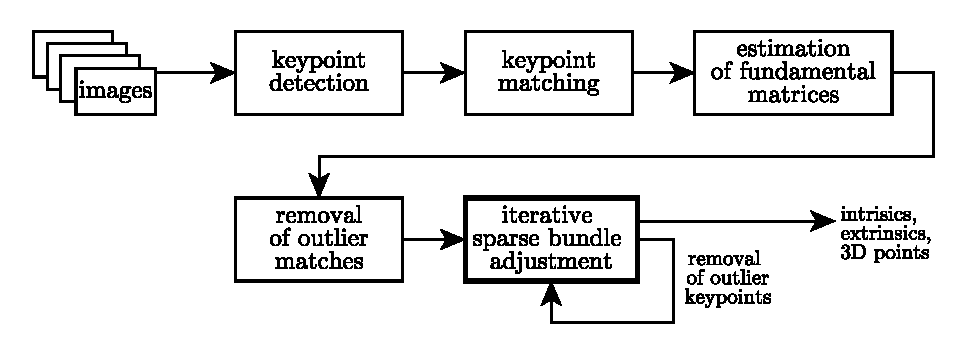
\includegraphics[width=0.8\textwidth]{fig/3d_reconstruction_pipeline.pdf}
	\caption{The 3D reconstruction pipeline taking multiple images obtained from uncalibrated cameras and producing estimated camera parameters and locations of matched points in 3-space.}
	\label{fig:3d_reconstruction_pipeline}
\end{figure}

The algorithm takes arbitrary number of images on the input and performs \textit{SIFT keypoint detection} as the first step. Next, individual keypoints are matched across all images creating the \textit{tracks}. A \textit{fundamental matrix $\matr{F}$} is estimated for each pair of images (see Section \ref{txt:epipolar_geometry}) and those matches which are outliers with regards to $\matr{F}$ are removed. Finally, the \textit{iterative sparse bundle adjustment} (see Section \ref{txt:bundle_adjustment}) which produces the estimates of camera parameters (both intrinsics and extrinsics) and 3D locations of matched points is run.

In case of the OLS both extrinsics and intrinsics are known. However, they are correct only up to a systematic and random error caused by imprecise stationing and rectification (see Chapter \ref{txt:precision_of_the_localization}) and a noise which the P\&T unit orientation measurements are subject to. Therefore, in order to achieve a 3D reconstruction of the surrounding environment it is still reasonable to employ the bundle adjustment technique. In order to exploit the a priori known information the bundle adjustment could be for instance initialized with known camera calibration and pose parameters so as to make the optimization algorithm more likely to find the global optimum.

%.........................................................................
%.........................................................................
\subsection{Epipolar Geometry} \label{txt:epipolar_geometry}

Epipolar geometry represents the relation between two projective pinhole cameras observing the same point (points) in 3-space \cite{Cyganek:2007:ICV:1214366} (see Figure \ref{fig:epipolar_geometry}). The line between both camera centers $\vec{C_{i}}$ is called the \textit{baseline} and it delimits the \textit{epipole} $ \vec{e_{i}}$ in each projective plane $Im_{i}$. The projection of target $\vec{T}$ to both image planes defines image points $\vec{t_{i}}$ which in return back-project to lines in 3-space. The line $el_{i}$ lying in image plane $Im_{i}$ connecting $\vec{e_{i}}$ and ${\vec{t_{i}}}$ is called the \textit{epipolar line}.

What the epipolar geometry relation says is that the observed target $\vec{T}$ must lie only in the plane $Ep$ defined by the baseline and both back-projected lines (from the camera center $\vec{C_{i}}$ through the image point $\vec{t_{i}}$). Alternatively, the epipolar line $el_{i}$ is the projection of back-projected line $\vec{C_{j}}\vec{t_{j}}$ to the projection plane $Im_{i}$.

%% Epipolar geometry
\begin{figure}[tbh]
	\centering
	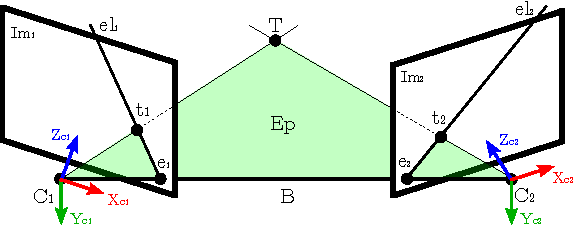
\includegraphics[width=0.7\textwidth]{fig/epipolar_geometry.pdf}
	\caption{The epipolar geometry.}
	\label{fig:epipolar_geometry}
\end{figure}

Ultimately, the \textit{epipolar constraint} is defined as following: \textit{Each image point $\vec{t_{i}}$ of a space point $\vec{T}$ lies in the image plane only on the corresponding epipolar line}. This can be stated numerically using the \textit{fundamental matrix} $\matr{F}$:
\begin{align}
	\vec{t_{1}}^{T}\matr{F}\vec{t_{2}} = 0
\end{align}

Fundamental matrix $\matr{F}$ can be estimated from mere image correspondences for instance using normalized 8-point algorithm within RANSAC framework \cite{Hartley:2003:MVG:861369, Cyganek:2007:ICV:1214366}.

%.........................................................................
%.........................................................................
\subsection{Bundle Adjustment} \label{txt:bundle_adjustment}

Bundle adjustment is the approach which aims to simultaneously refine the parameters of all involved cameras (intrinsics and extrinsics) and to minimize the reprojection error between the initially measured image point and reprojected target. The non-linear least squares error function $E$ can be defined as \cite{Forsyth:2002:CVM:580035}:
\begin{align}
	E = \frac{1}{mn}\sum_{i,j}{[(x_{ij} - \frac{\vec{p_{i1}}\vec{T_{j}}}{\vec{p_{i3}}\vec{T_{j}}})^{2} + (y_{ij} - \frac{\vec{p_{i2}}\vec{T_{j}}}{\vec{p_{i3}}\vec{T_{j}}})^{2}]},
\end{align}
where $m$ is the number of cameras, $n$ is the number of target points in 3-space, $(x_{ij}, y_{ij})$ is the initially measured location of the projection of target $T_{j}$ to the projective plane of camera $i$ and $\vec{p_{ir}}$ is the rth row of projection matrix $P_{i}$. As for the minimization, \textit{Levenberg-Marquardt} algorithm is mostly used. 

In case of reconstruction approach proposed by Snavely, Seitz and Szeliski \cite{Snavely:2006:PTE:1179352.1141964} (see Section \ref{txt:reconstruction_pipeline}) the iterative version of bundle adjustment is used. In this case the most suitable image pair which has enough matches and large baseline is selected and the camera parameters as well as the 3D locations of matched points are estimated. In each next iteration a new camera is added to the optimization algorithm.

%.........................................................................
%.........................................................................
\subsection{VisualSFM}

VisualSFM\footnote{Official website of VisualSFM: \url{http://ccwu.me/vsfm/index.html}} is a well established application for end-to-end scene reconstruction using multiple cameras which follows the standard pipeline described in Section \ref{fig:3d_reconstruction_pipeline} and adds another method for dense reconstruction. For sparse reconstruction the application uses parallel implementation of bundle adjustment \cite{ChangchangWu:2011:MBA:2191740.2191945} and for dense reconstruction the Patch-based Multi-view Stereo Software (PMVS) approach is utilized \cite{Furu:2010:PMVS}. The demonstration of dense reconstruction is depicted in Figure \ref{fig:visualsfm_tower}. Upon successful reconstruction the VisualSFM enables the 3D point cloud to be exported in standard PLY format which could be imported to the OLS for instance with the use of Point Cloud Library (see Section \ref{txt:occlusion_prediction}).

%% Visual SFM tower
\begin{figure}[tbh]
	\centering
	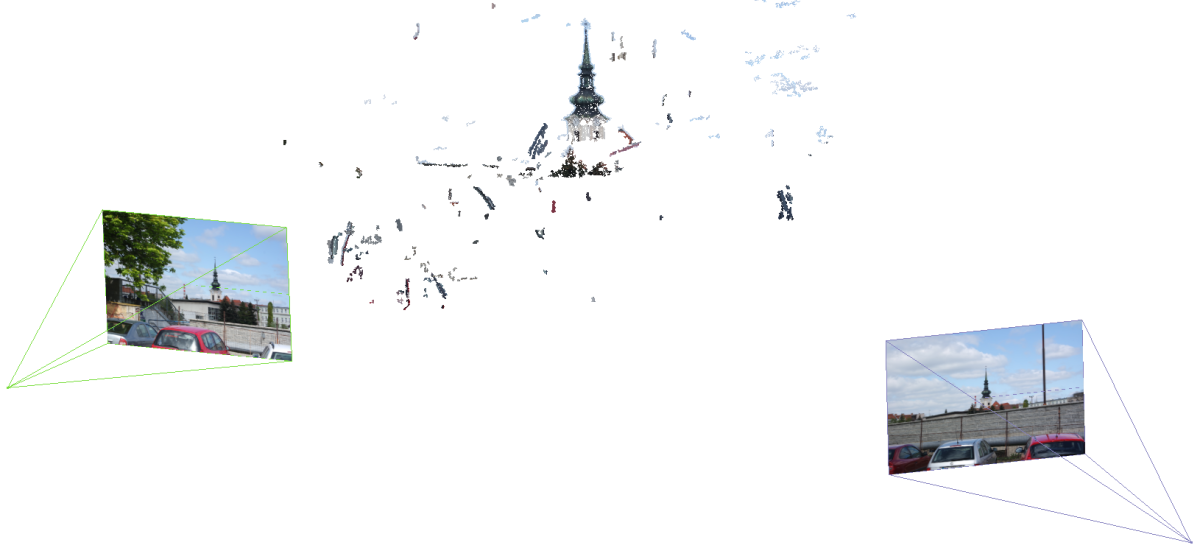
\includegraphics[width=0.9\textwidth]{fig/visualsfm_tower.png}
	\caption{The 3D reconstruction performed by VisualSFM from only two photographs taken by the same camera in district Štýřice (Brno, Czech Republic). Note that even mere two views suffice to reconstruct the church tower, however, the output data include a lot of noise.}
	\label{fig:visualsfm_tower}
\end{figure}

%=========================================================================
%=========================================================================
\chapter{Precision of the Localization in Multi-camera System} \label{txt:precision_of_the_localization}

The whole chapter is devoted to exploring the problematics of error analysis which must be performed prior to the system design. The objective is to find prospectively most severe sources of error already in the early stages of the system development and to take appropriate measures in order to eliminate them. First, the proposed topology of the OLS design so as to maximize the system precision is proposed and described in Section \ref{txt:system_topology}. Section \ref{txt:precision_analysis} then discusses the main sources of error in the system, categorizes them and provides a detailed analysis of impact each error poses on the OLS. Finally, Sections \ref{txt:stationing} and \ref{txt:rectification} explain the processes of \textit{stationing} and \textit{rectification} which aim on eliminating certain types of errors.

%-------------------------------------------------------------------------
%-------------------------------------------------------------------------
\section{System Topology} \label{txt:system_topology}

The main building block of the OLS is a \textit{camera unit} (CU) -- an independent collection of hardware modules including positionable camera and various sensors used for estimating the geographical coordinates of the CU itself (see Figure \ref{fig:cu_and_topology}). Detailed description of the CU will be given in Section \ref{txt:camera_unit}, however, for the purpose of precision analysis it suffice to remark that a camera which each CU is equipped with is free to rotate around azimuthal and elevation axes and it is used for the visual tracking of a target.

As was explained in Section \ref{txt:triangulation_with_noisy_measurements} a system consisting of at least two cameras is capable of estimating the position of the target in 3-space using triangulation. The main strength of the OLS is the fact it is designed to work with an arbitrary number of CUs, therefore the estimated position of the target can be refined by incorporating multiple hypotheses. As will be explained in Section \ref{txt:precision_analysis} the geometric limitations of the stereo-view systems significantly affect the localization precision. Therefore, the CUs should be positioned so that their positions projected to the horizontal plane would form approximately regular polygon. A sample setup of the OLS is depicted in Figure \ref{fig:cu_and_topology}.

%% Photograph of the CU.
%% Use case of camera units - placed on map of Brno's Spilberk
\begin{figure}[htb]\centering
	\centering
	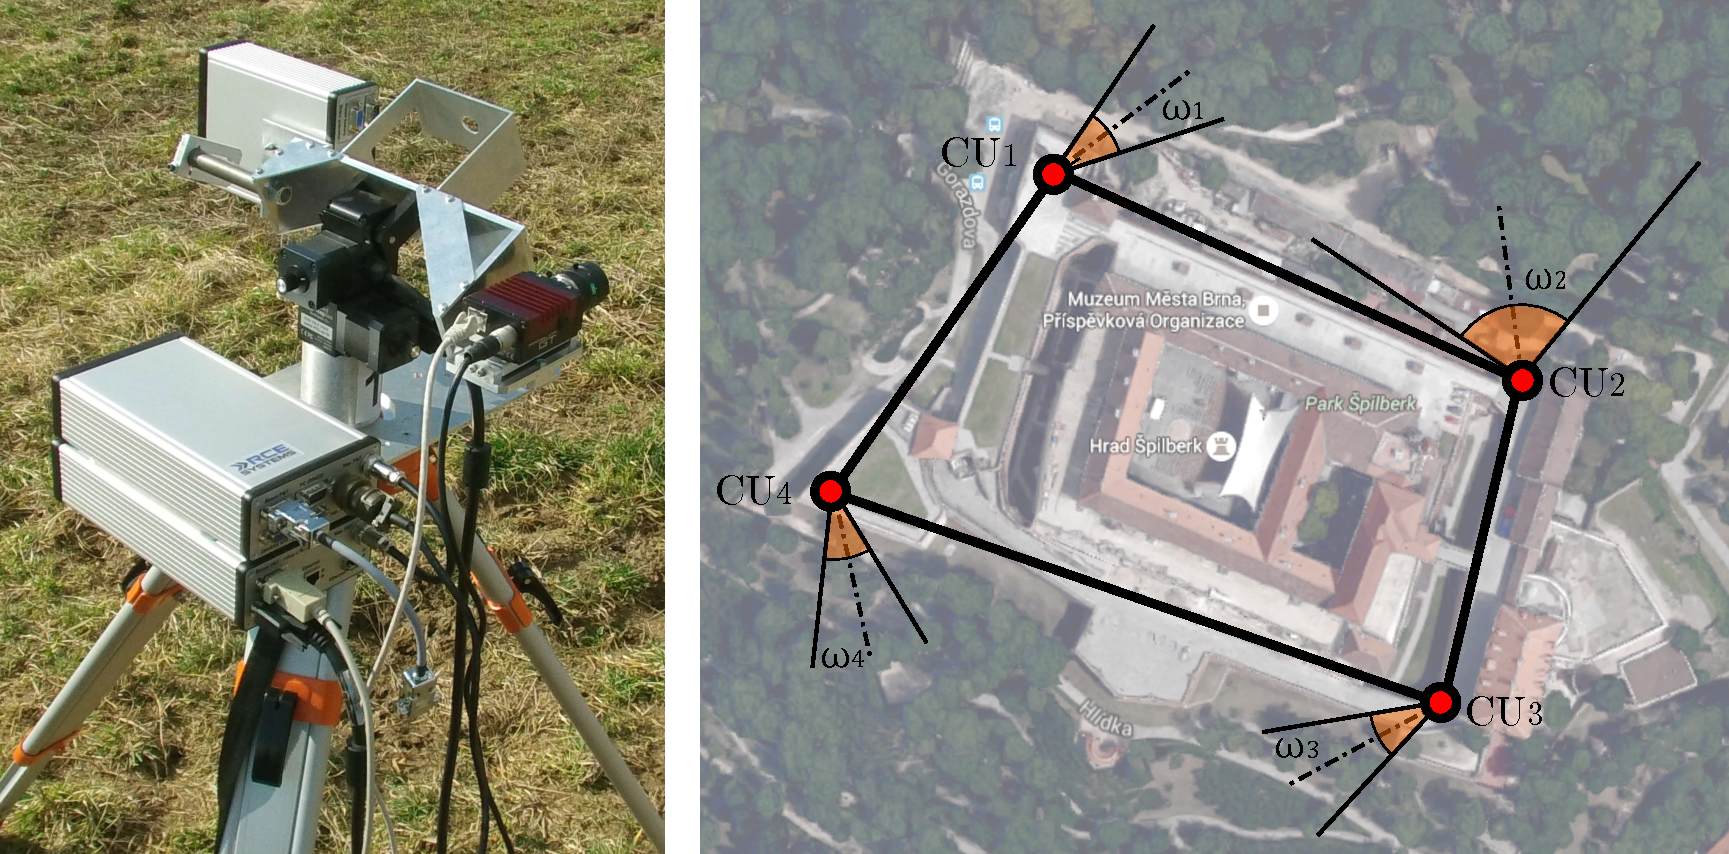
\includegraphics[width=0.75\linewidth]{fig/cu_and_spilberk_camera_units.pdf}
	\caption{The photograph of the CU (left) and a use case scenario (right) showing four CUs (red dots) positioned so as to protect a real world area (castle Špilberk in Brno, Czech Republic). Note that in general each camera might have different FOV depicted as an angle~$\omega$.}
	\label{fig:cu_and_topology}
\end{figure}

~\\
~\\
%-------------------------------------------------------------------------
%-------------------------------------------------------------------------
\section{Precision Analysis} \label{txt:precision_analysis}

The precision of the system can be defined in the means of the frame-by-frame Euclidean distance $E$ between the estimated location $\vec{T_{est}}$ and the real (ground truth) location $\vec{T_{GT}}$ of the tracked target:
\begin{align}
	E = \lVert \vec{T_{GT}} - \vec{T_{est}} \rVert.
\end{align}

Since the precision can be affected severely by multiple independent factors it is essential to perform the error analysis in order to discover and prospectively alleviate the most prominent contributors of the overall error.

%.........................................................................
%.........................................................................
\subsection{Sources of Error}

The precision of estimating the target position is subject to various types of errors which have different impact on the overall deflection. Basically, there two main categories of errors can be distinguished, the \textit{systematic error} and the \textit{random error} \cite{taylor1997introduction}.

\paragraph{Systematic error} The main property of systematic error is the fact that it cannot be revealed by repeating the measurement. I.e. this error is intrinsicly integrated in the system itself and it always distorts the measurements the same way. In case of the OLS the sources of the systematic error are the discrepancy between the physical CU and its model (imprecise mechanical construction) and imprecise stationing (i.e. finding the global orientation and geographical coordinates of each CU). In order to eliminate the systematic error in the OLS the process of stationing (see Section \ref{txt:stationing}) and rectification (see Section \ref{txt:rectification}) were designed.

\paragraph{Random error} This type of error can be usually described by a probability distribution i.e. it behaves in a random manner. As for the OLS the main source of random error is the visual tracker which typically outputs the measurements oscillating around the correct target position. This phenomenon is caused jointly by non-maturity of the tracking algorithms and by the clutter present in the environment such as the atmospheric turbulences or refractive index fluctuations. Another source of the random error are the measurements of the current azimuth and elevation of the P\&T unit and time synchronization among the cameras. The random error can be alleviated by making the visual tracker more robust (see Section \ref{txt:visual_tracking}).\\

Whether being systematic or random, in the OLS the error eventually reflects in undesirable rotation and/or translation of the CU model with regards to its real physical counterpart and consequently, when computing the triangulation the rays are back-projected in the wrong direction and/or from the wrong position. Note that given the nature of triangulation (see Section \ref{txt:triangulation}) the OLS is extremely sensitive to error angles (caused e.g. by wrong estimation of heading). Contrarily, the error translations (caused e.g. by faulty GPS measurement) are not of major concern (see Figure \ref{fig:rotation_vs_translation}).

%% Transaltion vs rotation error.
\begin{figure}[htb]\centering
	\centering
	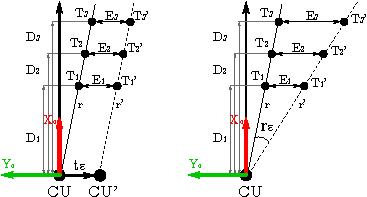
\includegraphics[width=0.55\linewidth]{fig/rotation_vs_translation.pdf}
	\caption{The impact of undesirable error translation $t_{\epsilon}$ (left) and error rotation angle $r_{\epsilon}$ (right) of the CU model which causes the back-projection of incorrect ray $r'$ instead of correct $r$. Note that in case of $t_{\epsilon}$ the localization error $E_{i}$ is invariant to the distance $D_{i}$ of target $T_{i}$. Contrarily, in case of $r_{\epsilon}$ the more distant the target $T_{i}$ is the higher value the localization error $E_{i}$ reaches.}
	\label{fig:rotation_vs_translation}
\end{figure}

%.........................................................................
%.........................................................................
\subsection{Error in Two-View System}

Stereoscopic systems are affected by a phenomenon of diminishing accuracy of depth measurement with increasing distance of the target from the cameras \cite{Cyganek:2007:ICV:1214366}. The depth measurement resolution for canonical stereo setup is:
\begin{align}
R = \frac{rd^{2}}{fB - rD},
\end{align}
where $f$ is the focal length, $B$ is the baseline length, $r$ is the horizontal size of one pixel and $D$ is the target distance. By substituting $r$ by $pr$, where $p$ is the random error represented by integer number of pixels we obtain the \textit{position estimation error function}
\begin{align}
E = \frac{prD^{2}}{fB - prD}.
\end{align}

The OLS does not conform to the canonical stereo setup (all cameras can rotate freely) so the dependence of the error on the target distance is no longer quadratic (considering the setup of two cameras where only one of them makes error): 
\begin{align}
E = B\tan(\arctan(\frac{D}{B}) + \arctan(\frac{r}{f})) - D.
\end{align}

The cameras setup as well as the error shown as the function of the baseline length and target distance is depicted in Figure \ref{fig:errorGivenBaseAndDistance}. Note that the higher the distance of the target and at the same time the lower the baseline length the higher the precision error.

\begin{figure}[htb]\centering
	\centering
	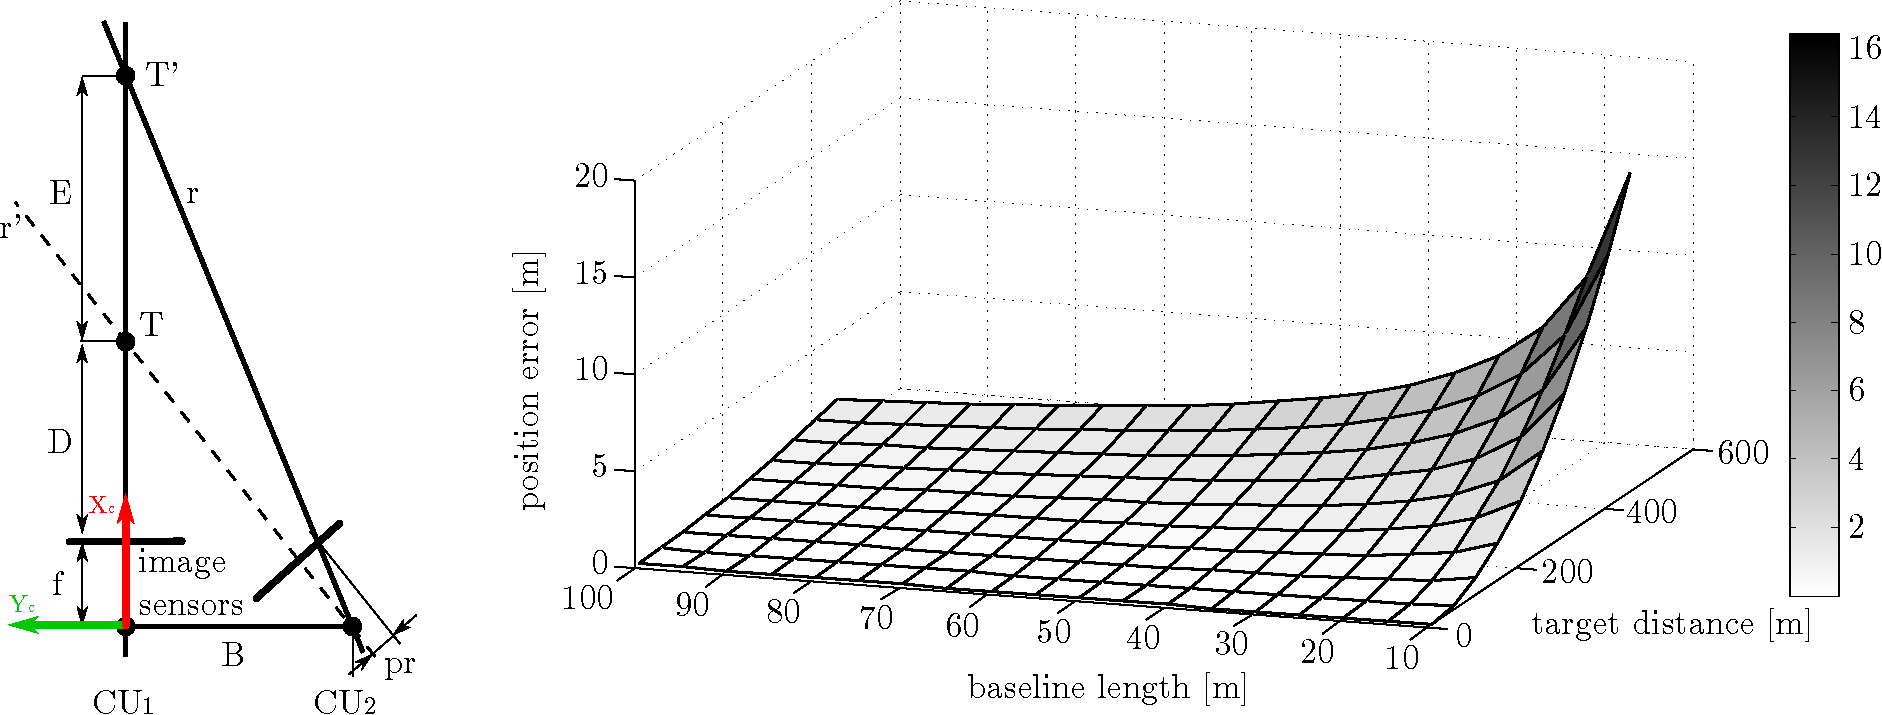
\includegraphics[width=0.9\linewidth]{fig/error_2_units_baseline_distance}
	\caption{Left figure depicts the setup of two cameras $CU_{1}$ and $CU_{2}$ where only $CU_{2}$ makes an error worth $p$ pixels. $T$ represents the ground truth position of the target whereas $T'$ is the wrongly estimated position. Right figure shows the position estimation error as the function of baseline length and the target distance (given the random error $p~=~10~px$ and following constants corresponding to the hardware used in the OLS: $r~=~3.75e^{-6}~m,\ f~=~50e^{-3}~m$).}
	\label{fig:errorGivenBaseAndDistance}
\end{figure}

%.........................................................................
%.........................................................................
\subsection{Error in Multiple-View System}

A more realistic scenario where each camera makes a random error $p$ is depicted in Figure \ref{fig:errorMapGivenTargetPosition}. A significant advantage of using multiple cameras is demonstrated --- the geometrical limitations of the two-camera setup make it impossible to precisely evaluate the position of the target placed close to the line collinear with the baseline (see Figure \ref{fig:target_base_geometry_and_worst_error}). In the multi-camera setup, on the other hand, the subset of two cameras forming the baseline $B_{i}$ is used for each position of the target, following the rule: 

\begin{align}
i = \argmax_{i}\ \vec{t_{i}}\vec{n_{i}},
\end{align}
where $\vec{t_{i}}$ is the direction of the line segment linking the center of the baseline $CU_{c}$ and the target and $n_{i}$ is the normal vector of the baseline $B_{i}$. Put in other way, the baseline $B_{i}$ yielding the highest absolute value of angle $\gamma$ is chosen to compute the position of the target.

% Target-base geometry.
% MEthodology of worst error estimation.
\begin{figure}[htb]\centering
	\centering
	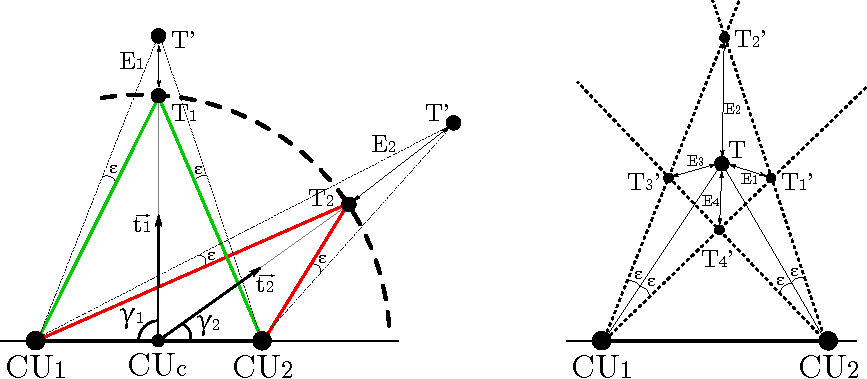
\includegraphics[width=0.75\linewidth]{fig/target_base_geometry.pdf}
	\caption{Left figure demonstrates the basic geometrical limitation of the two-view system which causes the position estimation error $E$ to increase rapidly as the angle $\gamma$ between the baseline and the target decrease up to the point where $\gamma$ is zero and $E$ becomes infinitely large. Note that both CUs make the same random error depicted as error angle $\epsilon$. Right figure shows four possible intersections of the rays back-projected from both CUs making random error given as the angle $\epsilon$. When analyzing the precision the worst error $E_{i}$ is always chosen.}
	\label{fig:target_base_geometry_and_worst_error}
\end{figure}

The Figure \ref{fig:errorMapGivenTargetPosition} depicts the position estimation error as the function of the target's position with regards to the CUs for both two-camera and three-camera setup. In this scenario only horizontal position of the target is considered (i.e. its height is disregarded) and it is assumed that each tracker makes the random error worth $p = 10~px$. For each position of the target the worst possible location estimation is considered (see Figure \ref{fig:target_base_geometry_and_worst_error}).

\begin{figure}[!htb]\centering
	\centering
	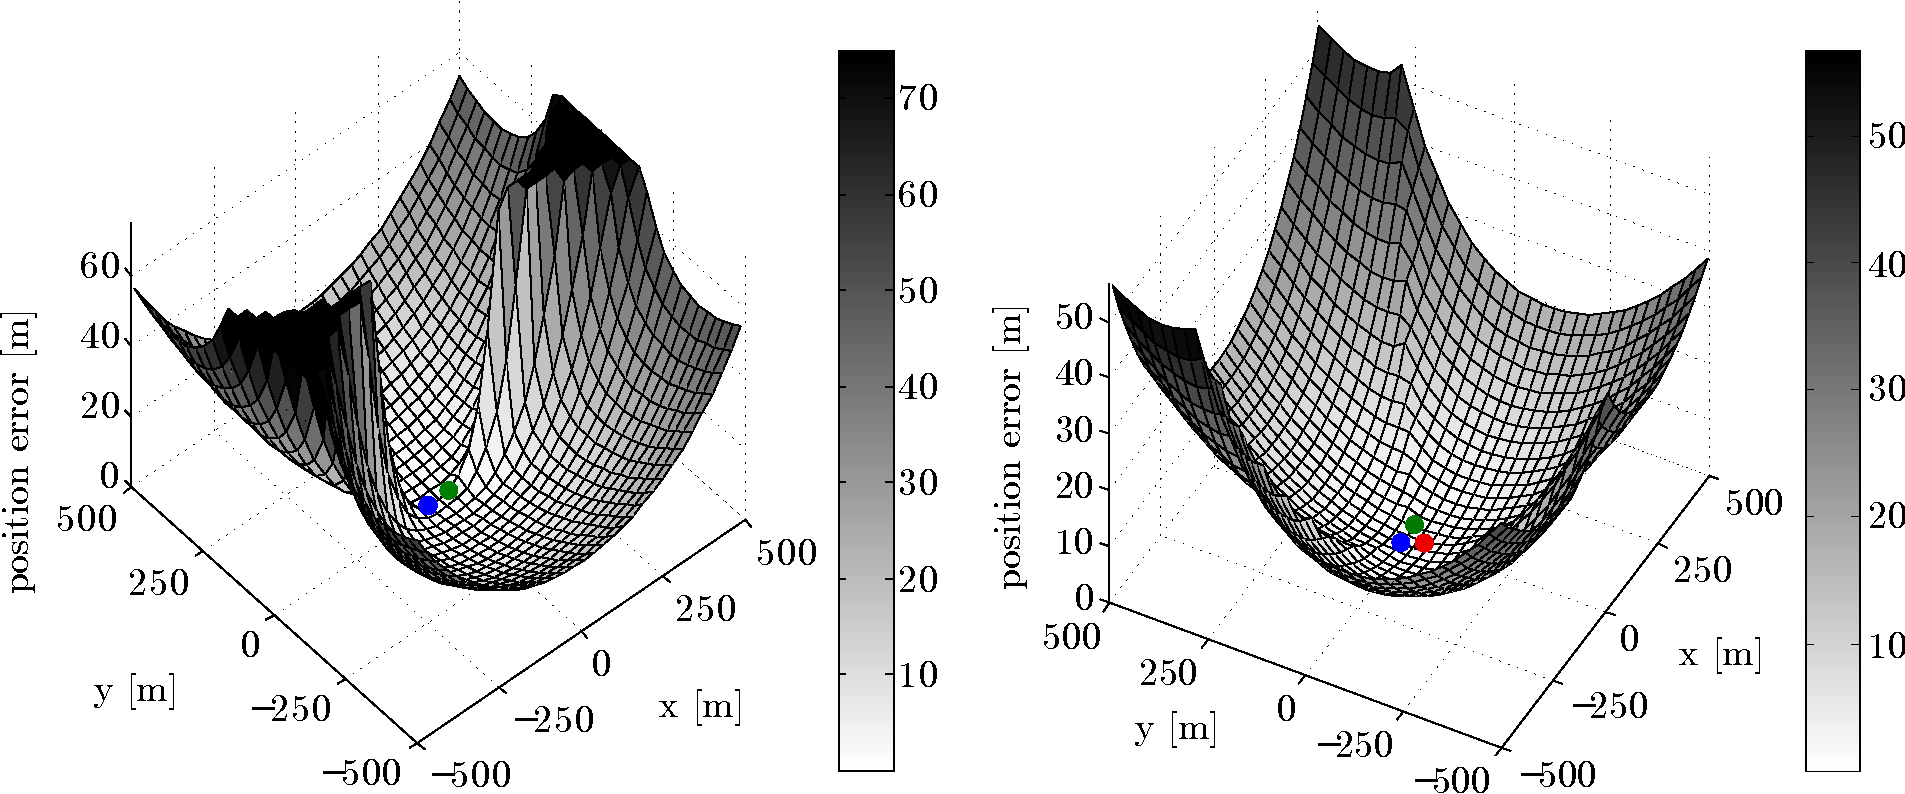
\includegraphics[width=0.95\linewidth]{fig/2_vs_3_cus.pdf}
	\caption{The position estimation error as the function of the horizontal position of the target. Two-camera (left) and three-camera (right) setup with $B = 20\ m$ are confronted where utilization of more cameras always yields lower errors. The first two cameras are placed on the X axis with the coordinate frame center in the middle of their baseline. The third camera is placed on the Y axis, so that all the cameras form a regular triangle.} 
	\label{fig:errorMapGivenTargetPosition}
\end{figure}


%-------------------------------------------------------------------------
%-------------------------------------------------------------------------
\section{Stationing} \label{txt:stationing}

The main purpose of the \textit{stationing} process is to find the positions and orientations of all CUs with regards to the global (world) coordinate system. The stationing consists of four subtasks: finding the global position (using DGPS sensor), ensuring horizontality, finding absolute heading\footnote{\textit{Heading} is the term used to describe the angle between the torso of the human body and the geographical north \cite{Henriksson648760}.} and finding relative heading. Great care should be taken when performing stationing since imprecise estimates of the position and/orientation are the main source of the systematic error which significantly impacts the overall localization precision of the system.

%.........................................................................
%.........................................................................
\subsection{Horizontality}
Since the CU is expected to be placed in an unknown outdoor terrain it will never stand on an ideally horizontal surface. Therefore, it is necessary to either ensure that the unevenness of the surface is compensated by the suitable setting of the CU's stand or both the side tilt and front tilt angles of the stand must be estimated and integrated to the CU model. For these purposes the inclinometer attached to the base plane of the camera unit (see Section~\ref{txt:camera_unit}) is used.

%.........................................................................
%.........................................................................
\subsection{Absolute Heading} \label{txt:absolute_heading}

Though it is a common practice to estimate the heading using a magnetometer, this device is unsuitable for the OLS since the accuracy of the current professional class magnetometers starts at ca $10~mrad$ \cite{Honeywell:compassing_catalog} which is insufficient.

In order to find the orientation of each camera unit placed in the outdoor environment, distinctive landmarks with known geographical positions are used. For each such landmark the P\&T unit is rotated so that the optical axis of the camera would intersect that landmark and the azimuth value is registered. Using triangulation the geographical position of the camera unit is derived.

A different possible approach takes advantage of the celestial objects such as the moon, sun or stars for which the current geographical position is known as well. Nevertheless, this approach can only be used between the sunset and the dawn.

%.........................................................................
%.........................................................................
\subsection{Relative Heading}

To further reduce the impact of both random error produced by the GPS sensor and the systematic error given by the imprecision of absolute heading estimation it is reasonable to find the relative heading of each camera unit with regards to the rest of the camera units. Furthermore, relative heading estimation is inevitable in case the absolute heading cannot be measured at all. In case of the OLS, the absolute heading was not measured during testing (see Section \ref{txt:real_world_testing}) and the system relied only on the relative hading estimation.

The process of relative heading estimation is run separately for each pair of CUs. First, the azimuth and elevation of both P\&T units is set so that the optical axis of the camera would intersect the expected location of the LED target of the other CU. Then the position is refined so that the camera would aim directly at the center of the LED target (see Figure \ref{fig:stationing_aiming}). Current azimuth and elevation values of both CUs are saved and the whole model of the system is updated accordingly.

%% Stationing process of one pair of the camera units
\begin{figure}[htb]
	\centering
	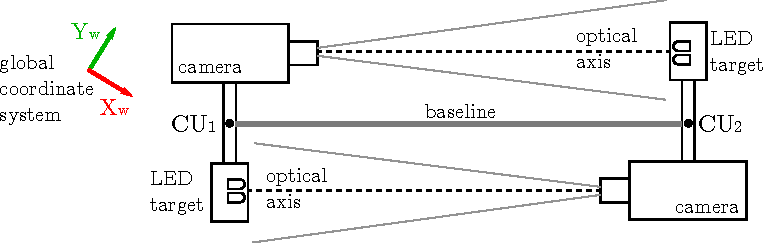
\includegraphics[width=0.7\linewidth]{fig/stationing.pdf}
	\caption{Schema of the stationing process where two CUs attempt to align the optical axes of their cameras.}
	\label{fig:stationing_aiming}
\end{figure}

%-------------------------------------------------------------------------
%-------------------------------------------------------------------------
\section{Rectification} \label{txt:rectification}

The \textit{rectification} process serves the purpose of reducing the systematic error caused by the imprecise attachment of the camera to the P\&T unit. The objective is to fix the camera in such a position that the image sensor becomes parallel  with both azimuthal and elevation axis. At the same time the rows of the image sensor must remain parallel with the elevation axis (i.e. the camera is not rotated around the optical axis). If it is not possible to fix the camera precisely in required position (mechanical limitations of the camera mount) the error angles must be measured and integrated to the CU model. The rectification process consists of three parts: \textit{eliminating rotation along the optical axis}, \textit{measuring rotation along the azimuthal axis} and \textit{finding the default elevation angle}.

%.........................................................................
%.........................................................................
\subsection{Eliminating Rotation Along the Optical Axis}

The camera is attached to a custom made metal mount. The mount itself is then attached to the P\&T unit using two opposing round tenons enabling for the rotation around the axis parallel with the optical axis of the camera (see Figure \ref{fig:rect_model_front_view}).

%% The front view of the model of the camera unit
\begin{figure}[htb]
	\centering
	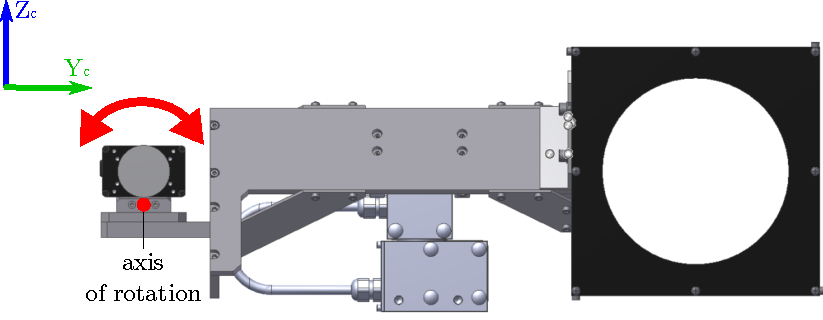
\includegraphics[width=10cm]{fig/rect_model_front_view.pdf}
	\caption{Front view of the top part of the CU. The red arrow denotes the possible rotation of the camera along the axis parallel to the optical axis. Image courtesy of company Oprox, a.s.}
	\label{fig:rect_model_front_view}
\end{figure}

In this part the rectification target with three parallel horizontal black lines is used. As the first step a surveying automatic level is used to rotate the target so that the black lines become horizontal. The camera is then positioned so as to aim approximately at the center of the target. The camera image stream is blended with the same stream mirrored across the vertical axis. Finally, the objective is to manually rotate the camera so that the black lines in blended image stream appear visually aligned (see Figure \ref{fig:rect_mirrored_stream}). Once set, the mount with the camera is fixed to the manipulator using two set screws.

%% Rectification of the rows of the camera image sensor - original stream blended with the mirrored stream
\begin{figure}[htb]
	\centering
	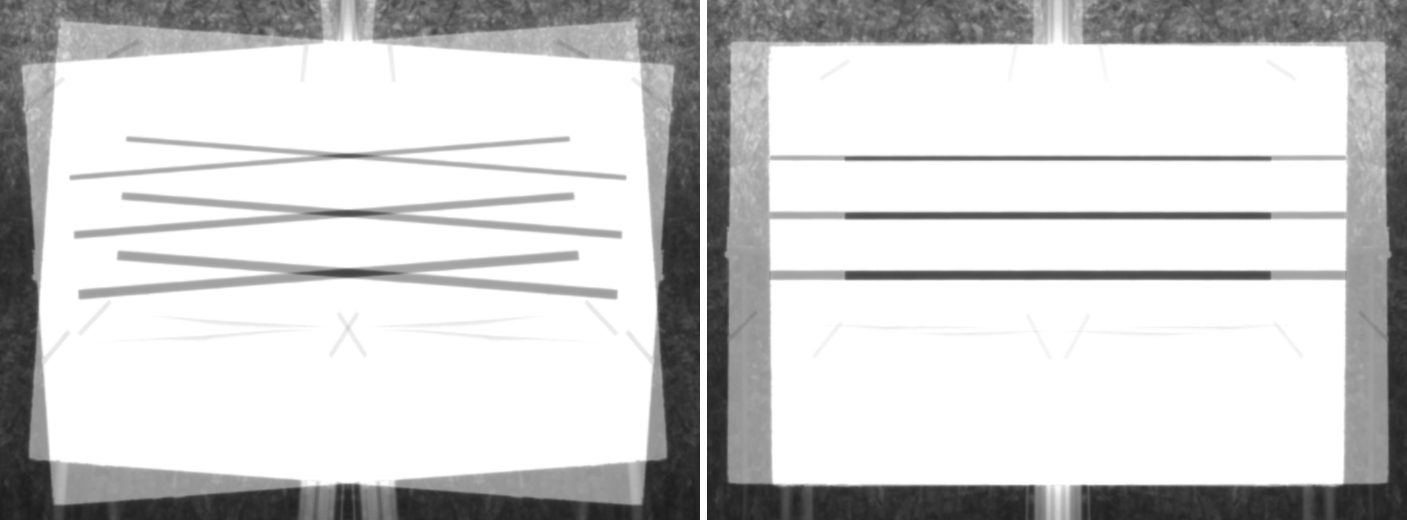
\includegraphics[width=0.75\textwidth]{fig/rect_mirrored_stream.png}
	\caption{A blended image stream from the camera before (left) and after (right) rotating the camera along the optical axis to the correct position.}
	\label{fig:rect_mirrored_stream}
\end{figure}

%.........................................................................
%.........................................................................
\subsection{Measuring Rotation Along the Azimuthal Axis}

The mount can still rotate around the axis parallel with the azimuthal axis (see Figure \ref{fig:rect_model_top_view}). It is necessary to ensure that the optical axis of the camera is perpendicular to the elevation axis. The same target from the first part of the rectification is used but two black crosses are added to the selected horizontal black line. The distance $d_{ao}\ m$ between two crosses equals to the distance between the azimuthal and optical axis (which is known from the engineering design, see Figure \ref{fig:rect_azi_axis}).

%% The top view of the model of the camera unit
\begin{figure}[htb]
	\centering
	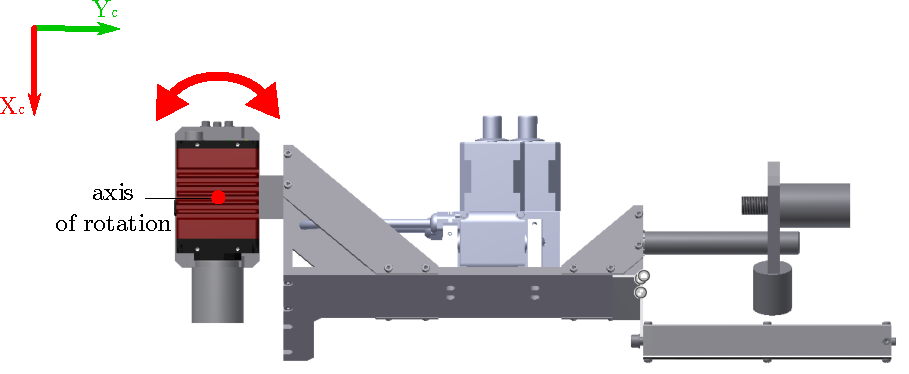
\includegraphics[width=11cm]{fig/rect_model_top_view.pdf}
	\caption{Top view of the top part of the CU. The red arrow shows the possible rotation of the camera along the axis parallel to the azimuthal axis. Image courtesy of company Oprox, a.s.}
	\label{fig:rect_model_top_view}
\end{figure}

A military monocular telescope (see Figure \ref{fig:rect_telescope}) is mounted on top of the manipulator. The optical axis of the telescope intersects the azimuthal axis, it is perpendicular to it and it intersects the left cross of a given pair on the rectification target. The camera is rotated so that its optical axis intersects the right cross and then it is fixed using set screws. As the screws are tightened the camera is unintentionally rotated a bit again which causes the visual offset between the crosshair and the cross on the target. The offset $d_{h}$ expressed in pixels is transformed to the default rotation angle $\beta$ (see Figure \ref{fig:rect_pixel_offset}) of the joint \textsc{camera} in the CU model:

\begin{equation}
\begin{aligned}
\beta &= \arctan\frac{d_{h}cs}{f},
\end{aligned}
\end{equation}
where $f$ is the focal length and $cs$ is the physical size of one pixel.

%% Photograph of the camera unit with the telescope mounted on the top
%% Screenshot of the digital crosshair and the offset
\begin{figure}[htb]
	\centering
	\begin{minipage}{.37\textwidth}
		\centering
		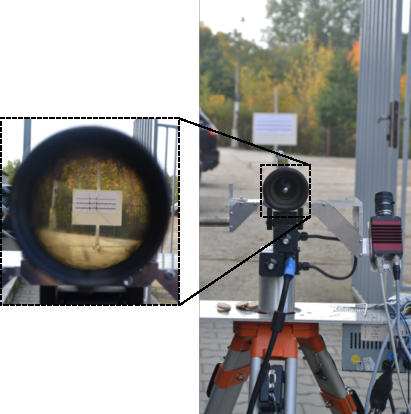
\includegraphics[width=.99\linewidth]{fig/rect_telescope.pdf}
		\captionof{figure}{A telescope mounted on top of the P\&T unit. A person looking through a telescope sees the black crosshair.}
		\label{fig:rect_telescope}
	\end{minipage}
	\hfill
	\begin{minipage}{.59\textwidth}
		\centering
		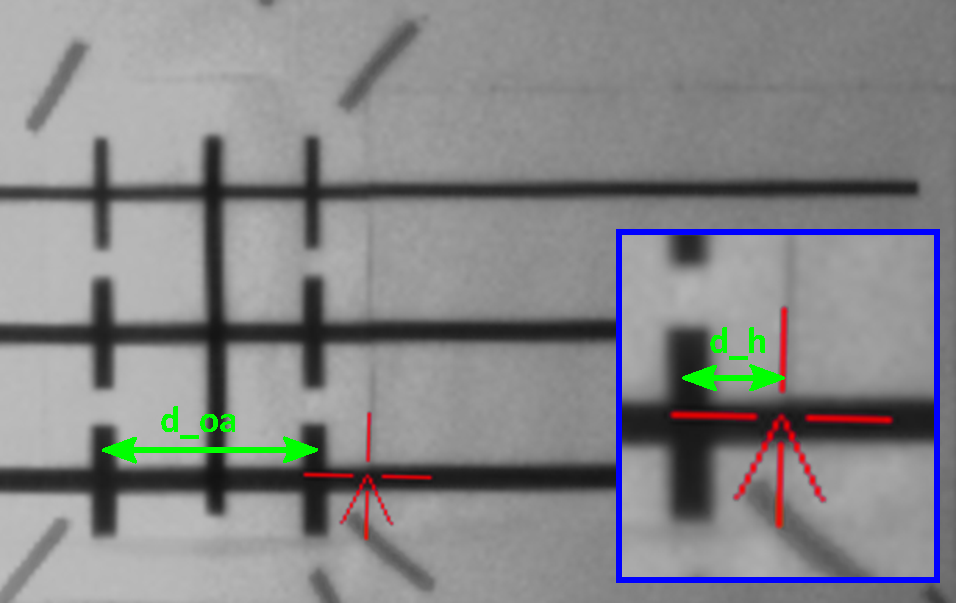
\includegraphics[width=.99\linewidth]{fig/rect_azi_axis.pdf}
		\captionof{figure}{Rectification target with the pairs of black crosses. The two crosses in a pair are $d_{ao}\ m$ apart. A digital crosshair is displayed in order to find the horizontal offset $d_{h}$.}
		\label{fig:rect_azi_axis}
	\end{minipage}
\end{figure}




%% Geometry schema showing how to calculate angle beta - pixel offset
\begin{figure}[htb]
	\centering
	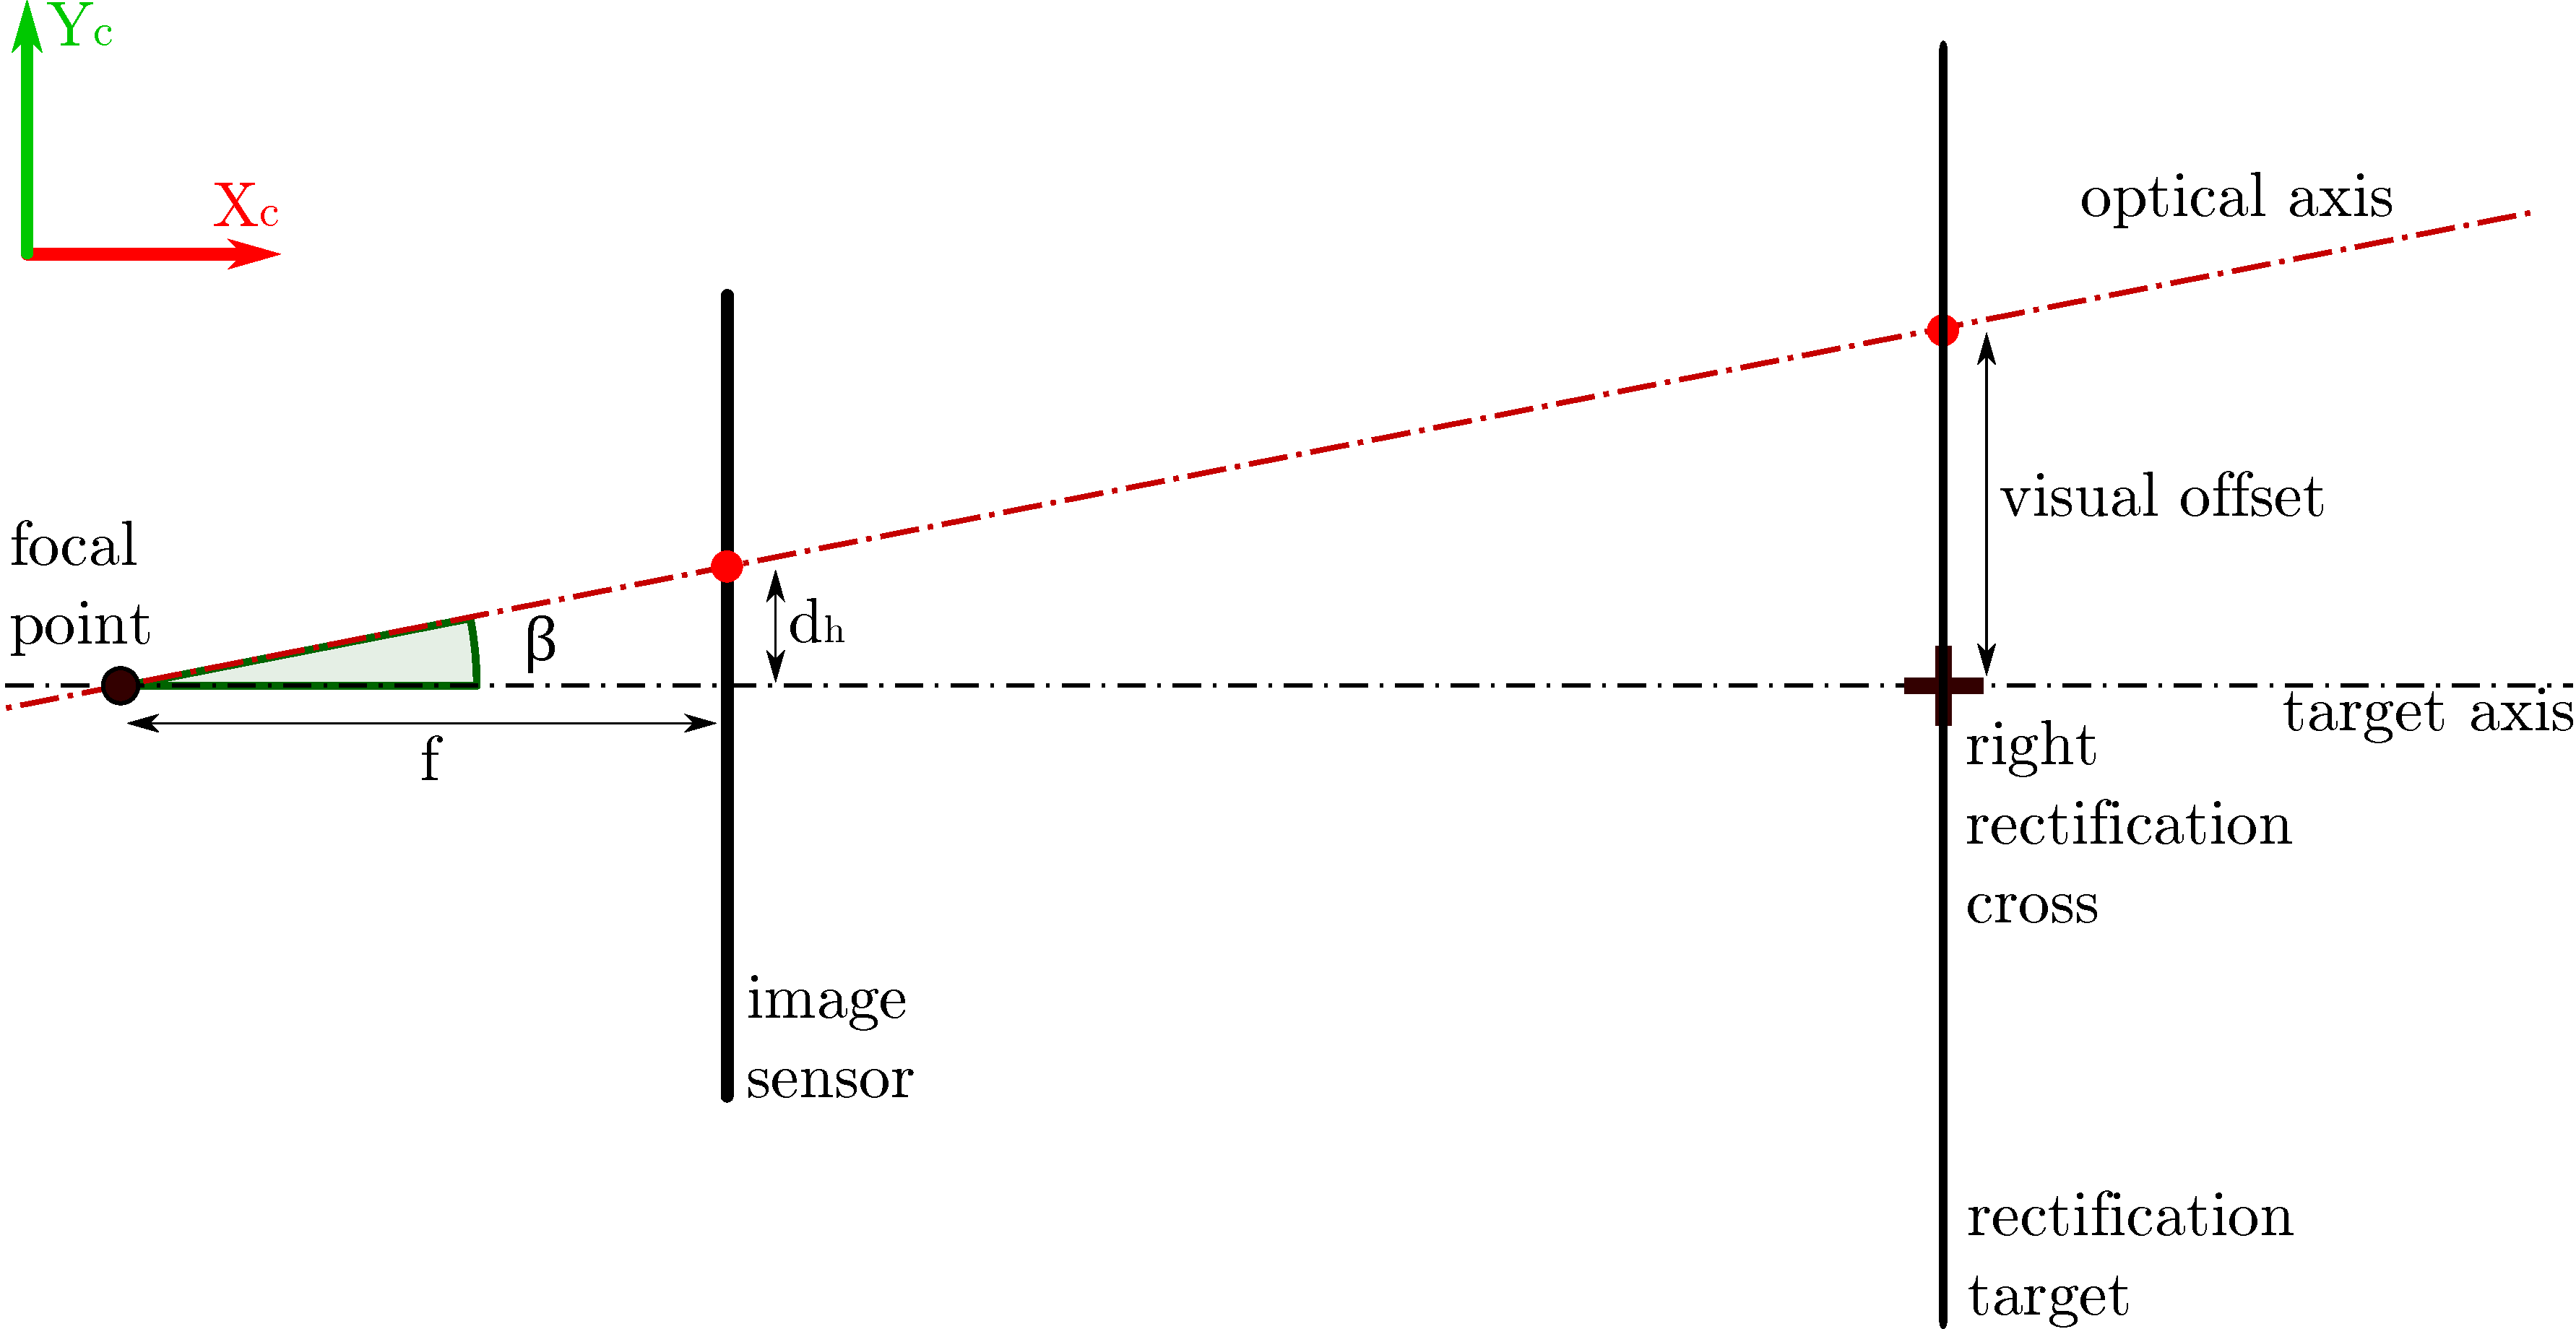
\includegraphics[width=0.65\linewidth]{fig/rect_pixel_offset.pdf}
	\caption{The top view schema of a rectification target being projected to the image sensor of the camera.}
	\label{fig:rect_pixel_offset}
\end{figure}


%.........................................................................
%.........................................................................
\subsection{Finding the Default Elevation Angle}

Considering the limited elevation range of the P\&T unit \texttt{Flir PTU D46-70} (see Section \ref{txt:camera_unit}) the camera must be mounted pre-rotated around the elevation axis by approximately $-60^{\circ}$. However, after fixing the camera it is necessary to find this default angle precisely. 

For this purpose a pair of rectification targets which consist of horizontal black and white lines representing the marks of a ruler are used. The targets are positioned in a row with the distance of a few meters so that the front target would overlap approximately half of the rare target when observed from the camera. The operator manually adjusts the elevation of the manipulator until the digital crosshair intersects the same mark on both targets where the two marks form a straight line (see figure \ref{fig:rect_default_elevation_angle}). Once such an elevation is found the angle is recorded and integrated to the model of the camera unit as an angle of rotation around the Y-axis of the joint \textsc{camera} (see Section \ref{txt:camera_unit}).

%% The rectification target for finding the default elevation angle.
\begin{figure}[htb]
	\centering
	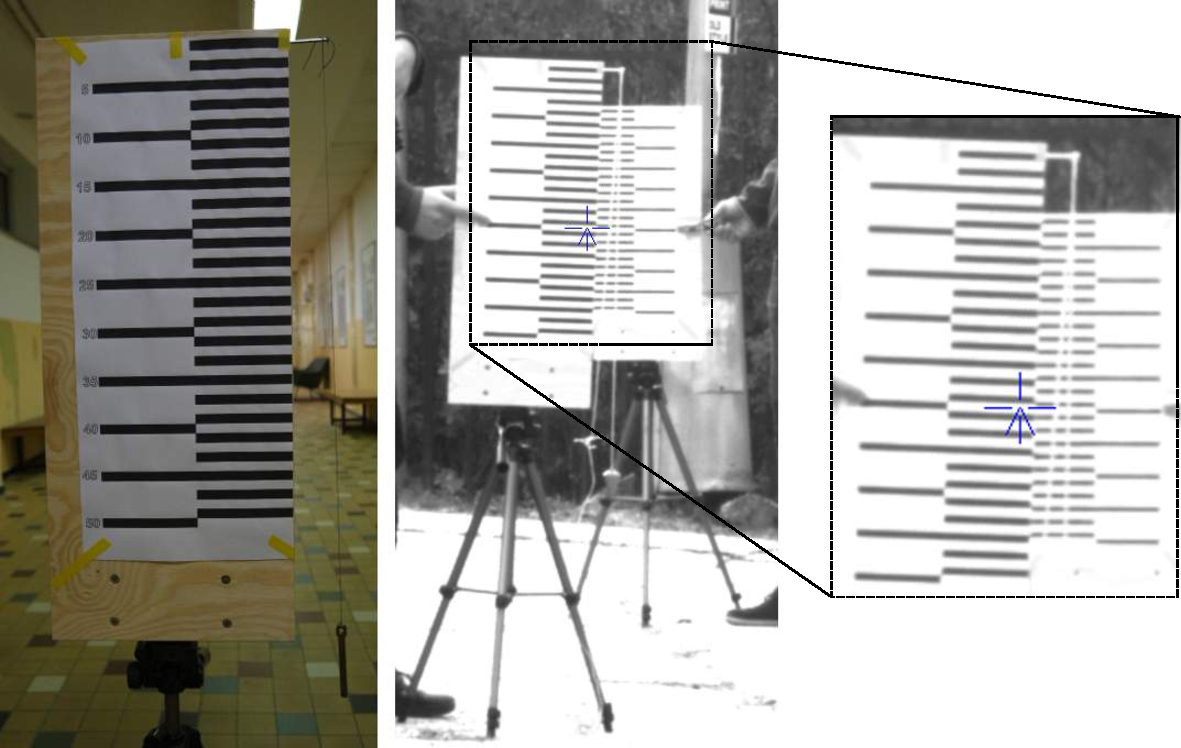
\includegraphics[width=13cm]{fig/rect_default_elevation_angle.pdf}
	\caption{Front target of a pair of the rectification targets used to find a default elevation angle (left). A screenshot from the image stream of the camera with the crosshair focused on a row where the marks of the rulers align (right).}
	\label{fig:rect_default_elevation_angle}
\end{figure}


%=========================================================================
%=========================================================================
\chapter{Design of the Optical Localization System} \label{txt:design_of_the_OLS}

This chapter describes the overall design of the OLS from both hardware and software perspective. First, the main physical component of the system -- the camera unit -- is presented. The hardware components which the camera unit consists of are described and the suitable model based on the kinematic chain is proposed in Section \ref{txt:camera_unit}. Next Section \ref{txt:visual_tracking} delves into the specific requirements and proposed solutions for the visual tracking. The Section \ref{txt:target_localization_using_triangulation} explains the proposed approach to localizing the target in multi-view scenario given the noisy measurements and Section \ref{txt:occlusion_prediction} describes the proposed approach to utilize the 3D model of the environment in order to predict the occlusion. Finally, Section \ref{txt:hw_and_sw_architecture} presents both hardware and software architecture of the system.

%-------------------------------------------------------------------------
%-------------------------------------------------------------------------
\section{Camera Unit} \label{txt:camera_unit}

As stated in Section \ref{txt:system_topology} the main component of the OLS is a camera unit (CU). Basically, the CU consists of hardware devices necessary for capturing the images, for manipulating the pose of the camera, for estimating absolute geographical position and orientation of the station as well as relative position and orientation with regards to the rest of the stations and for running the OLS software.

There are two type of CUs. The \textit{overview unit} is designed to be controlled manually by the human operator and it is equipped with the zooming lens that allows achieving both a wider scanning range and a more detailed view of the farther objects. The \textit{tracking unit} consists of the fixed lens and takes part in the autonomous tracking of the moving objects and continuous reporting of the estimated directions towards the target.

The hardware components used for tracking stations are described in greater detail in Section \ref{txt:devices}. In order to triangulate the target, the 3D location of the camera as well as the direction of the optical axis must be known for each captured frame, thus a suitable model corresponding to the real hardware mus be designed. Proposed model based on the kinematic chain is introduced in Section \ref{txt:model}.

%-------------------------------------------------------------------------
%-------------------------------------------------------------------------
\subsection{Devices and Components} \label{txt:devices}

The CU (see Figure \ref{fig:camera_unit_photo_model}) consists of a surveying tripod providing a solid base on which a manipulator (P\&T unit\footnote{From English Pan and Tilt.}), a camera and all of the devices used for stationing (LED target, GPS sensor and inclinometer) are mounted. Each CU is equipped with its own desktop computer for processing the image data and calculating the 3D position estimates.

%% A photo of a camera unit and an rviz model.
\begin{figure}[tbh]
	\centering
	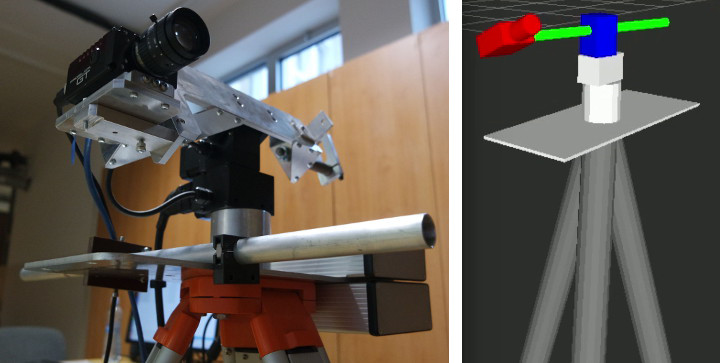
\includegraphics[width=10cm]{fig/camera_unit_photo_model.jpg}
	\caption{A photograph (left) of the upper part of the camera unit consisting of a manipulator Flir PTU-D46-70 with the aluminum mount carrying a camera Prosilica GT 1290C and a corresponding 3D model (right) created for \textit{rviz} and \textit{Gazebo} simulator (see Section~\ref{txt:application_of_gazebo}).}
	\label{fig:camera_unit_photo_model}
\end{figure}

\paragraph{Manipulator Flir PTU-D46-70} A manipulator PTU D46-70\footnote{Website of the product Flir PTU-D46-70: \url{http://www.flir.com/mcs/view/?id=53712}} produced by manufacturer Flir is used (see Figure \ref{fig:prosilica_gt1290c_flir_ptud4670}). As compared to the other professional manipulators this is a lower middle class device consisting of two stepper motors (pan and tilt axes). The device is capable of maximal angular speed of $60^{\circ}/s$ with the resolution of $0.003^{\circ}$ while the payload must not exceed $4.08~kg$ \cite{Flir_ptud4670}. The operational range is limited to $[-180^{\circ}, 180^{\circ}]$ in azimuth and $[-47^{\circ}, 80^{\circ}]$ in elevation. The manipulator incorporates no position feedback, the position is inferred from the number of steps and the current resolution, thus it is necessary not to overload the manipulator, otherwise it could loose synchrony and report wrong position.

\paragraph{Camera Prosilica GT 1290C} Prosilica GT 1290C\footnote{Website of the product Prosilica GT 1290C: \url{https://www.alliedvision.com/en/products/cameras/detail/1290-1.html}} is an industrial camera manufactured by the company Allied Vision (see Figure \ref{fig:prosilica_gt1290c_flir_ptud4670}). It is an RGB camera equipped with CCD sensor (type 1/3'') with the resolution of $1280 \times 960$ px and support for $33.3$ FPS and it communicates through gigabit Ethernet \cite{Prosilica_gt1290c}. What is important, the camera natively supports the Precision Time Protocol (PTP) for precise time synchronization which is a crucial feature in each application relying on stereo vision and it is capable of time synchronization among devices within the range of nanoseconds \cite{PTP}. The manufacturer claims that Prosilica GT 1290C achieves the synchronization precision of $1~\mu s$.

\paragraph{Lens Computar M5018-MP2} Each camera mounted on a tracking unit is equipped with a fixed-focus lens Computar M5018-MP2\footnote{Website of the product Computar M5018-MP2: \url{http://computar.com/product/556/M5018-MP2}} (see Figure \ref{fig:prosilica_gt1290c_flir_ptud4670}). The focal length $50~mm$ was chosen as a most suitable trade-off between the wide field of view and capability of imaging distant targets. Given the camera sensor type 1/3'' the effective horizontal field of view $fov_{h}$ is approximately $5.5^{\circ}$.

%% Photos of Flir and Prosilica.
\begin{figure}[htb]
	\centering
	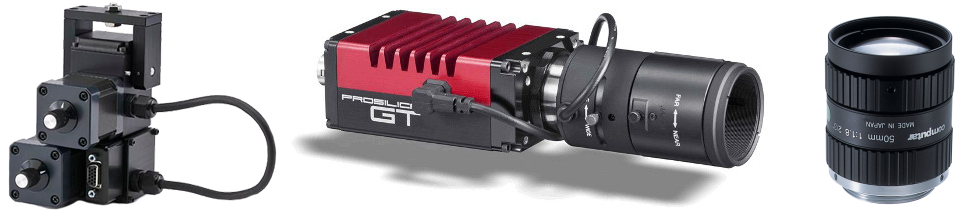
\includegraphics[width=0.9\linewidth]{fig/prosilica_gt1290c_flir_ptud4670_computar.png}
	\caption{Product pictures of manipulator Flir PTU D46-70 (left), camera Prosilica GT 1290C (middle) and lens Computar M5018-MP2 (right).}
	\label{fig:prosilica_gt1290c_flir_ptud4670}
\end{figure}

%-------------------------------------------------------------------------
%-------------------------------------------------------------------------
\subsection{Model} \label{txt:model}

The model of the camera unit is based on the kinematic chain consisting of six joints and five links corresponding to the distance between separate parts of the surveying tripod and separate parts of the manipulator (see Figure \ref{fig:camera_unit_kinematic_chain}). The starting joint \textsc{ground} itself is dependent on the reference location (let us call it \textsc{origin}) which represents the origin of the global coordinate frame. The transformation between \textsc{origin} and \textsc{ground} reflects the position and orientation of the given manipulator within the environment (which is estimated during the stationing process, see Section \ref{txt:stationing}).

The kinematic chain is designed as the composition of transformation matrices where a single joint can be located as a solution to the \textit{forward kinematics problem}, i.e. by applying the Euclidean transformation on the position of the joint it is dependent on. For instance the transformation matrix $M_{cam}$ of the joint \textsc{camera} can be derived as:

\begin{equation}
M_{cam} = M_{ele}T_{cam}R_{Z_{cam}}R_{X_{cam}}R_{Y_{cam}},
\end{equation}
where $M_{ele}$ is the transformation matrix of the joint \textsc{ele} which the joint \textsc{camera} is dependent on, and $T_{cam}$ and $R_{AXIS_{cam}}$ are transformation and rotation matrices describing transformation from the joint \textsc{ele} to the joint \textsc{camera}. 

Note that from the implementation point of view the OLS is built on the ROS framework (see Chapter \ref{txt:implementation}) which presents certain conventions, most importantly the orientation of the coordinate frame which is used throughout the document (see Figure \ref{fig:frame_convention}).

%% ROS frame conventions
\begin{figure}[htb]
	\centering
	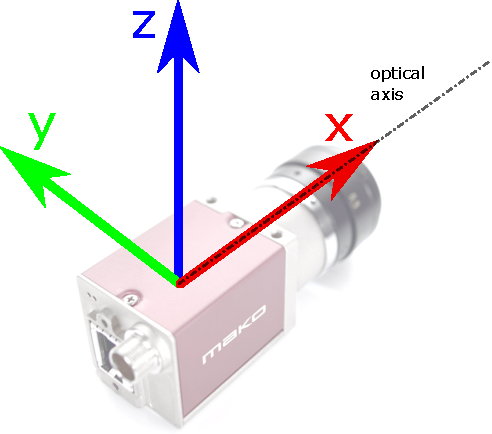
\includegraphics[width=0.2\linewidth]{fig/frame_convention.pdf}
	\caption{Frame orientation convention which is used throughout the work --- a right handed coordinate system with X axis aiming forward, Y axis aiming left and Z axis aiming up.}
	\label{fig:frame_convention}
\end{figure}

%% A schema of the camera unit - kinematic chain.
\begin{figure}[htb]
	\centering
	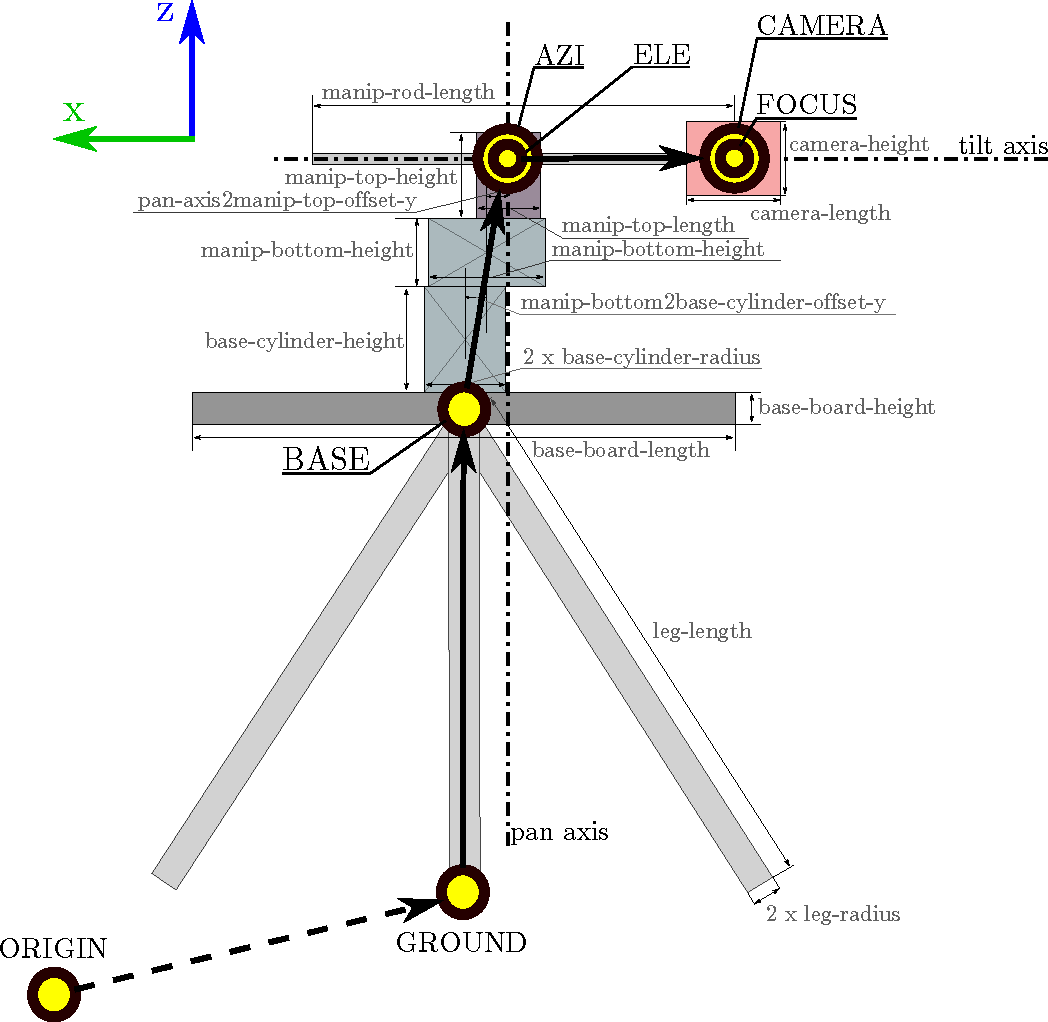
\includegraphics[width=0.6\linewidth]{fig/camera_unit_kinematic_chain.pdf}
	\caption{Schematic view of the kinematic chain of a camera unit with the joints depicted by the yellow circles. The sizes of all components necessary to specify the translation matrices between consecutive joints are shown as well. Note that this is the rear view, i.e. the camera is seen from behind. Thus the joints \textsc{camera} and \textsc{focus} overlap as they both lie on the optical axis (the joint \textsc{focus} has a lower value of the Z coordinate).}
	\label{fig:camera_unit_kinematic_chain}
\end{figure}


%-------------------------------------------------------------------------
%-------------------------------------------------------------------------
\section{Visual Tracking} \label{txt:visual_tracking}

The visual tracking subsystem of the OLS is based on the TLD tracker (\ref{txt:tracking_learning_detection}) and the BGFG tracker (\ref{txt:bgfg_tracker}). As explained in Section \ref{txt:precision_of_the_localization} the system is subject to multiple different sources of error which influence the precision of localization. As far as the visual tracking is concerned, the random error caused mostly by the common difficulties such as the background clutter, varying illumination, target appearance change etc. (see Section \ref{txt:object_model}) is of the most significance. Furthermore, in the worst case scenario the tracker might fail completely and never recover unless the human operator interferes.

Therefore, the BGFG tracker was adjusted so as to assign a belief to each measurement which then enables the localization subsystem to combine the measurements in the weighted manner (see Section \ref{txt:measurement_belief}). Furthermore, the bootstrap particle filter (BPF) algorithm of the BGFG tracker was adjusted so as to alleviate the failures caused by the harsh camera motion (see Section \ref{txt:adjusting_prediction_step}). Finally, the most suitable strategy for regulating the motion of the manipulator based on predicting the 2D motion of the target is proposed (see Section \ref{txt:2d_motion_prediction_and_regulation}).

%.........................................................................
%.........................................................................
\subsection{Measurement Belief} \label{txt:measurement_belief}

Since the OLS is designed as multi-camera system, the random error or failure of a single tracker might be compensated by the rest of the units; consequently the total impact on the localization precision is alleviated. In order to denote the certainty of the measurements coming from individual trackers the notion of \textit{belief} is introduced for the BGFG tracker (the operation of the BGFG tracker is described in Section \ref{txt:bgfg_tracker}).

The \textit{belief} is calculated for each frame and it is based on the distance function (\ref{eq:bgfg_distance_function}) which BGFG tracker uses to evaluate the candidate states represented by the particles. Basically, the distance function corresponds to the visual similarity of two image patches -- the target template and current candidate weighted by its foreground mask. Therefore, the particle weight is normalized by the maximum possible similarity so as to obtain a percent value \textit{belief} representing the similarity (i.e. $\textit{belief} \in [0, 1]$):
\begin{align}
	belief = \frac{\sum_{(x,y) \in I}{e^{min(M_{t}^{(x,y)}, M_{c}^{(x,y)})}(1 - |I_{t}^{(x,y)} - I_{c}^{(x,y)}|)^{2}}}{\sum_{(x,y) \in I}{e^{min(M_{t}^{(x,y)}, M_{c}^{(x,y)})}}},
\end{align}

Therefore, the noisy measurements or a complete failure of the tracker can be detected and propagated to the rest of the system (see Figure \ref{fig:belief}).

%% Comparison of template-candidate match and resulting belief.
\begin{figure}[htb]
	\centering
	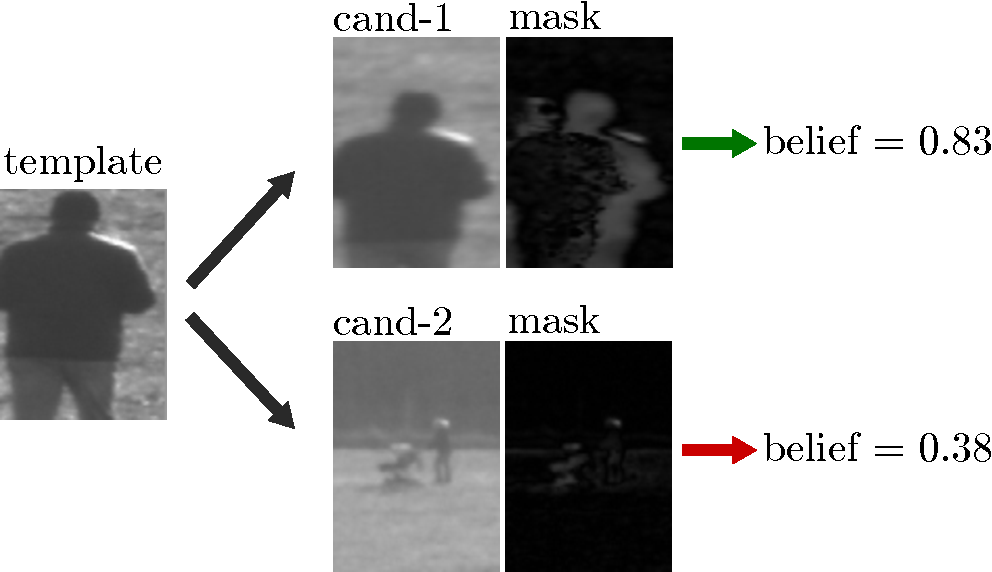
\includegraphics[width=0.5\linewidth]{fig/belief.pdf}
	\caption{The demonstration of the belief computed for two different candidates (top, bottom) given the input target template (left).}
	\label{fig:belief}
\end{figure}

%.........................................................................
%.........................................................................
\subsection{Adjusting Prediction Step Using Frame Differencing} \label{txt:adjusting_prediction_step}

One of the most common reasons for failure of the BGFG tracker is sudden and harsh motion of the camera mounted to the P\&T unit. In such a case the tracked target represented as a 2D location on the image plane of the camera abruptly changes its 2D position. The BGFG tracker continuously computes the homography \cite{ObjectTrackinginMonochromaticVideo} in order to detect the camera motion and incorporates it to the motion model of the target. However, the homography computation often fails mostly when the background is too uniform (e.g. a monotone field, a sky, etc.).

To deal with such cases, the BGFG tracker was adjusted so that in the \textit{prediction} step of the BPF a subset of particles would be forced to take the image positions yielding the highest response of the frame differencing computed for subsequent frames. Such locations are expected to contain the moving target of interest. As compared to the original \textit{prediction} step (\ref{eq:bgfg_pos_prediction}), the parameters $pos_{dim_{n}}^{i}$ representing 2D position of the particle $i$ in the dimension $dim$ (i.e. $x$ or $y$) in time $n$ takes the following form:
\begin{align}
	pos_{dim_{n+1}}^{i} =
	\begin{cases}
		fd_{dim_{n}} + x, ~ x \sim \mathcal{N}(\mu_{pos}, \sigma_{pos}),  & \text{if}\ FD_{max_{n}} \textgreater T \land i \textless M \\
		pos_{n}^{i} + x, ~ x \sim \mathcal{N}(\mu_{pos}, \sigma_{pos}), & \text{otherwise},
	\end{cases}
\end{align}

where $fd_{dim_{n}}$ is the coordinate of maximal intensity $F_{max_{n}}$ of the frame differencing in dimension $dim$ in time $n$, $T$ is the threshold which alleviates the ubiquitous non-zero frame differencing response caused by noise and $M$ is the number of particles which are allowed to change their position. Note that the particles are sorted according to their current weights in the ascending order, i.e. the index $i$ and constant $M$ denote whether the particle is allowed to change its position. The impact of adjusted \textit{prediction} step is depicted in Figure \ref{fig:frame_diff}. 

%% Adjusting update step in particle filter by response of frame differencing.
\begin{figure}[htb]
	\centering
	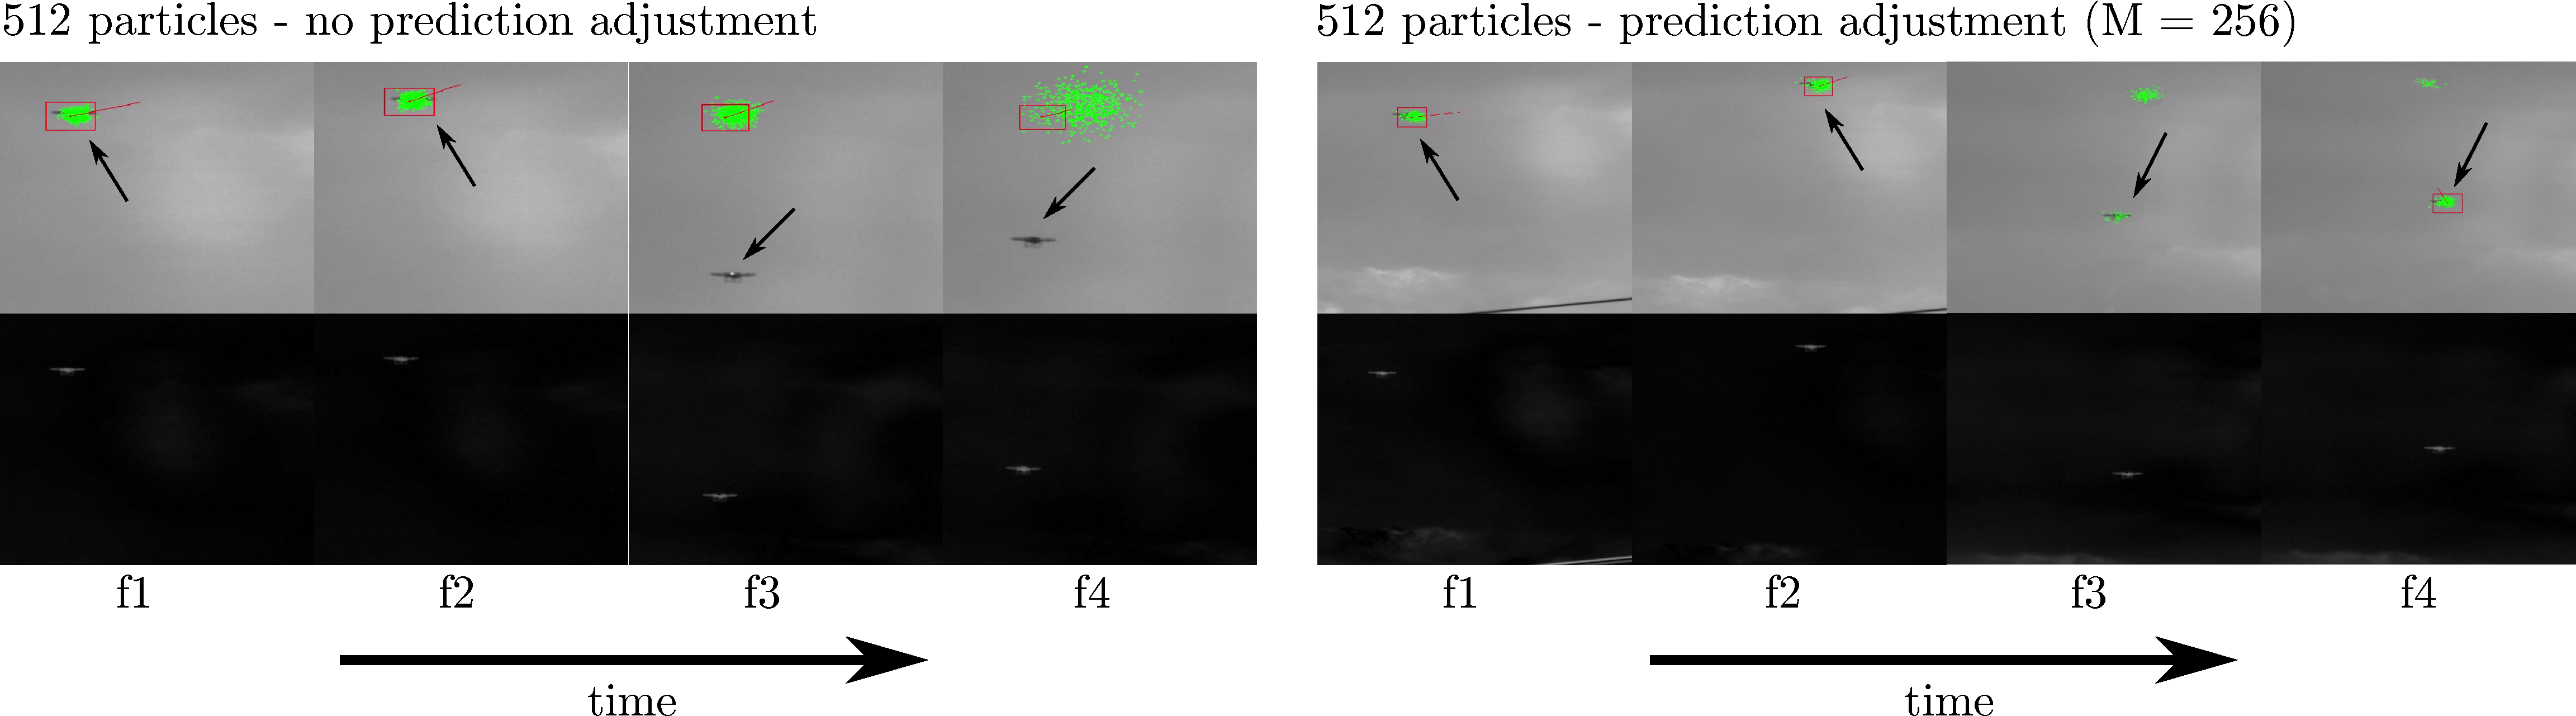
\includegraphics[width=0.99\linewidth]{fig/frame_diff.pdf}
	\caption{Four frames from two tracking sequences of the BGFG tracker are shown where the original (left) and adjusted (right) \textit{prediction step} implementation is used. The distribution of the particles (green dots) is manifested in the top row, the response of the frame differencing is shown in the bottom row. In both cases the tilt of the camera changes abruptly between frames $f 2$ and $f 3$ which causes the target (denoted by black arrow) to appear in the significantly different position. In the first scenario the particles fail to follow the target whereas in second scenario the subset of particles are forced to the position of the highest frame differencing response and consequently the target is found again.}
	\label{fig:frame_diff}
\end{figure}

%.........................................................................
%.........................................................................
\subsection{2D Motion Prediction and Regulation} \label{txt:2d_motion_prediction_and_regulation}

In order not to loose the moving target from the field of view the manipulator has to rotate the camera around both azimuthal and elevation axis appropriately. A most straightforward approach would be to simply measure the angular distance between the current measurement (i.e. the projection of the target to the image plane) and the center of the image and instruct the manipulator to move so as to minimize this distance as fast as possible. However, this approach is not sufficient. 

Contrarily, there are two main reasons why it is necessary to predict the future 2D position of the target. First, it is desirable to keep the target as close to the center of the image as possible so that there would be enough time to react in case of the sudden and rapid movement of the target. Second, the measurements are delayed (due to the tracking algorithm computation and communication delay) and the P\&T unit manifests considerable latency.

Given the time stamped ($t$) states of the manipulator $\vec{m} = (\phi, \psi)$ where $\phi$ and $\psi$ are the angular positions (given in $radians$) and tracker measurements $\vec{p} = (x, y)$, where $x$ and $y$ are the positions of the target (given in $pixels$), the 2D angular speed of the target $\vec{\omega_{t}}$ can be estimated as the moving average over $N$ last measurements $i$ as well as the angular difference $\vec{d} = (\phi_{diff}, \psi_{diff})$ between current and future 2D position in $T$ seconds:

\begin{align}
	\vec{\omega_{t}} &= \frac{\sum_{i=0}^{N-2}{\alpha(\vec{p_{i+1}} - \vec{p_{i}}) + (\vec{m_{i+1}} - \vec{m_{i}})}}{\sum_{i=0}^{N-2}{t_{i+1} - t_{i}}},\\
	\vec{d} &= \vec{\omega_{t}}T,
\end{align}
where $\alpha = \arctan{(\frac{cs}{f})}$ is the angular difference given by one \textit{pixel} which can be computed with the knowledge of the physical size of one pixel $cs$ and focal length $f$.

Then the manipulator can be instructed to move so as to reach the given angular distance $\vec{d}$. It is necessary that the angular speed $\vec{\omega_{m}}$ of the manipulator decreases gradually and smoothly as the target position is approached since the harsh motion of the camera might causes the failure of the tracker (see Section \ref{txt:adjusting_prediction_step}).

Due to the fact the tracker measurements and consequently the motion commands sent to the manipulator are delayed, the regulation function must define a \textit{deadzone}, i.e. the minimal angular distance $d_{min}$ to the target from which the manipulator is instructed to stop, otherwise it would oscillate in the vicinity of the static target indefinitely. The angular distance $d_{max}$ then defines the maximal desired \textit{cutoff} angular speed $\omega_{m_{max}}$ of the manipulator. The regulation function is then given as follows:

\begin{align}
	\omega_{m} &=
	\begin{cases}
		0,  & \text{if}\ d \textless d_{min}\\
		f_{reg},  & \text{if}\ d_{min} \leq d \textless d_{max}\\
		\omega_{max}, & \text{otherwise},
	\end{cases}
\end{align}
where $f_{reg}$ is either linear ($f_{lin} = ax+b$) or power ($f_{pow} = ax^{k}+b$) function. The example of a linear and power regulation function is depicted in figure \ref{fig:regulation_lin_power}.

%% Linear and power regulation functions.
\begin{figure}[htb]
	\centering
	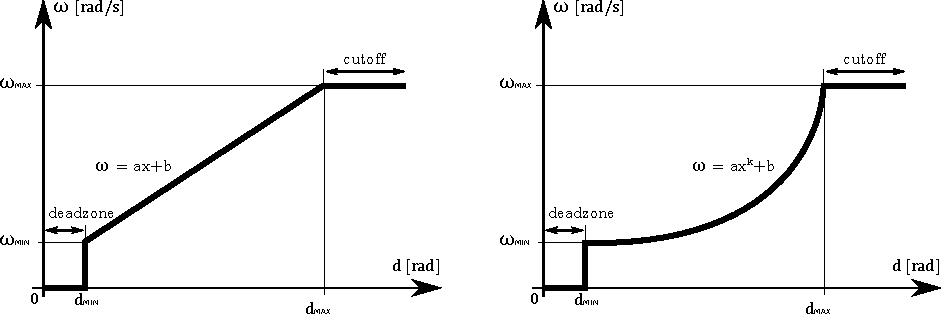
\includegraphics[width=0.75\linewidth]{fig/regulation_linear_power.pdf}
	\caption{The linear and power regulation function used for controlling the angular speed of the manipulator in the given dimension (azimuth or elevation).}
	\label{fig:regulation_lin_power}
\end{figure}

%-------------------------------------------------------------------------
%-------------------------------------------------------------------------
\section{Target Localization Using Triangulation} \label{txt:target_localization_using_triangulation}

This section describes the proposed triangulation method in two-view scenario (see Section \ref{txt:triangulation}), the incorporation of the a priori known relationship between the target-baseline orientation and the localization precision (see Section \ref{txt:incorporating_target-base_geometry}) and the strategy for estimating the speed and future locations of the target (see Section \ref{txt:3d_motion_predicition}).

%.........................................................................
%.........................................................................
\subsection{Triangulation} \label{txt:triangulation}

As explained in Section \ref{txt:multi_camera_target_localization} the position of the target in 3-space as seen by the stereoscopic system with known cameras' parameters can be calculated using triangulation. In case od the OLS the intrinsics were estimated for each camera during calibration and extrinsics are known at each time thanks to the sensory data streamed from the manipulators. However, due to the random and systematic error the rays back-projected from each camera might not intersect in the 3D space (see Figure \ref{fig:triangulationSchematicView}). Therefore, the common plane for both back-projected rays must first be found.

The estimation of the 3D position of the target consists of the following steps. First, back-projection is used to find the vectors $\vec{u}$ and $\vec{v}$ which form the planes $C_{1}C_{2}U$ and $C_{1}C_{2}V$ with the angle $\alpha$ between them. Both vectors are then rotated around the axis $\vec{m}$ so that they lie in the same plane $C_{1}C_{2}W$: $\vec{u'} = R(\beta_{1})\vec{u}$, $\vec{v'} = R(\beta_{2})\vec{v}$. The rotation angles $\beta_{1}$ and $\beta_{2}$ correspond to the beliefs $bel_{1}$ and $bel_{2}$ obtained from both trackers: $|\beta_{1}| = |\alpha|\frac{bel_{2}}{bel_{1} + bel_{2}},~|\beta_{2}| = |\alpha| -\beta_{1}$. Finally, the intersection $W$ of the vectors $\vec{u'}$ and $\vec{v'}$ is found.

% Triangulation with noisy measurements in 2-view system.
\begin{figure}[htb]\centering
	\centering
	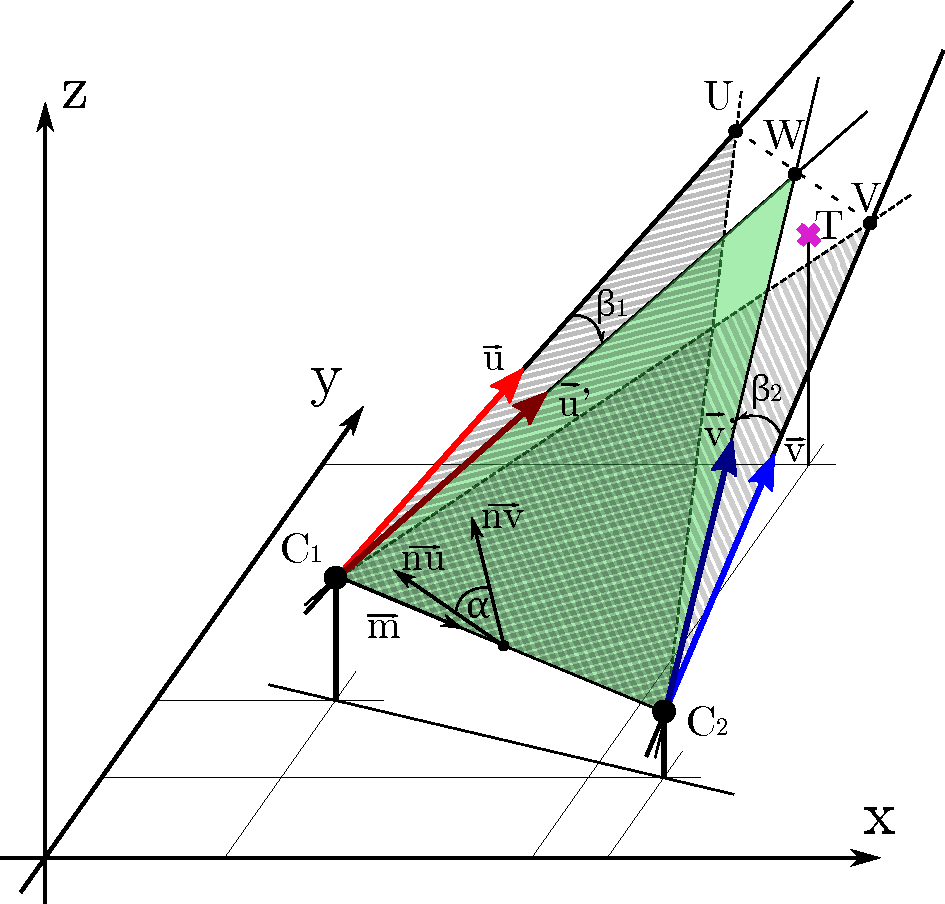
\includegraphics[width=0.45\linewidth]{fig/triangulation.pdf}
	\caption{A schematic view of a problem of 3D position estimation using triangulation in two-camera scenario. The camera units $C_{1}$ and $C_{2}$ observe the target $T$ in the directions $\vec{u}$ and $\vec{v}$. The plane $C_{1}C_{2}W$ is used as a common plane where the projected vectors $\vec{u'}$ and $\vec{v'}$ intersect.}
	\label{fig:triangulationSchematicView}
\end{figure}

%.........................................................................
%.........................................................................
\subsection{Incorporating Target-Base Geometry} \label{txt:incorporating_target-base_geometry}

If multiple CUs are used, the location of the target in 3-space can be estimated as the weighted centroid of the estimates $T_{i}$ computed by each pair of the camera units forming the baseline $b_{i}$. The weights correspond to the angle $\gamma$ between the baseline $b_{i}$ and the line intersecting the initially estimated position of the target $T'$ and the baseline center $bc_{i}$ since this angle significantly affects the localization precision (see Section \ref{txt:precision_of_the_localization}).

Basically, the location of the target in 3-space is estimated twice. First estimation $T'$ corresponds to the standard centroid of the individual estimates $T_{i}$. The second estimation refines the position $T'$ by using the weights corresponding to the target-baseline geometry (see Algorithm \ref{alg:3dPosEstimation}). The demonstration of the three-view scenario is shown in Figure \ref{fig:target-base_and_weighted_centroid}.

% Target-base geometry and weighted centroid computation
\begin{figure}[htb]\centering
	\centering
	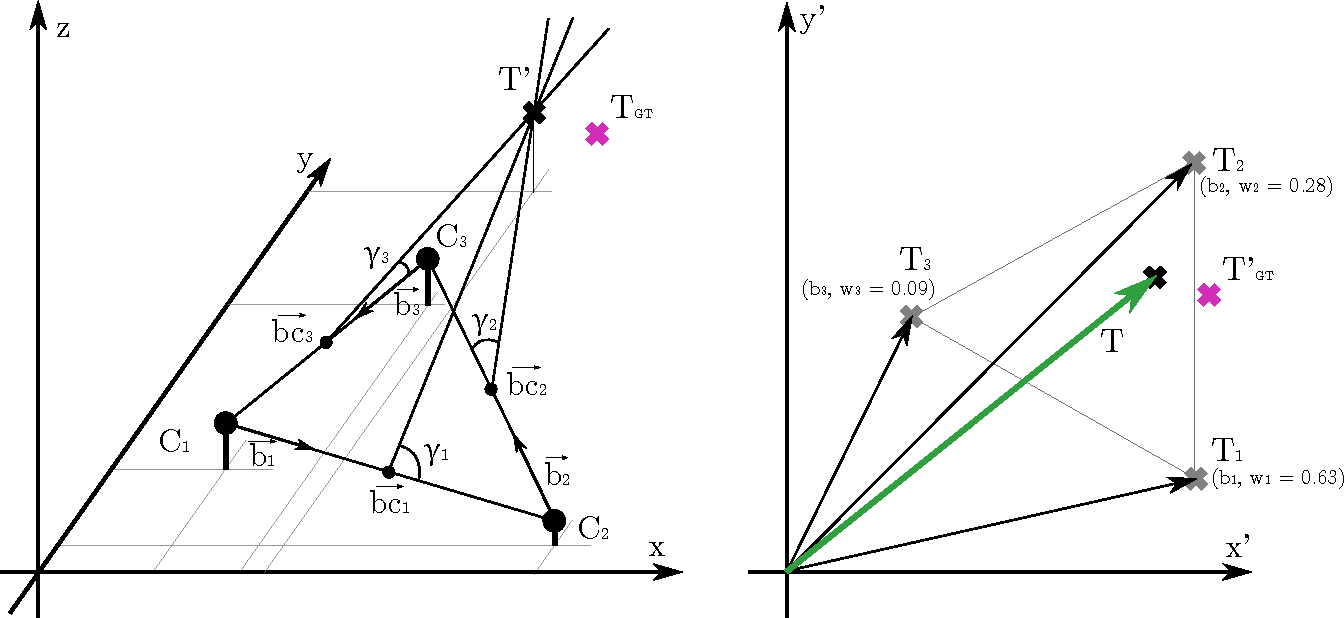
\includegraphics[width=0.8\linewidth]{fig/target-base_and_weighted_centroid.pdf}
	\caption{Left figure depicts the initial estimation of the target-baseline angles $\gamma_{i}$ in three-view localization scenario with the target $T_{GT}$. The right figure demonstrates the final estimation of the target location using the weights $w_{i} \sim \gamma_{i}$.}
	\label{fig:target-base_and_weighted_centroid}
\end{figure}

\begin{algorithm}
	\SetAlgoNoLine	
	\KwIn{Set of bases $B = {b_{1}, b_{2}, ..., b_{N}}$.}
	\KwOut{3D position estimate $T$.}
	\DontPrintSemicolon
	\BlankLine
	
	\SetCommentSty{textnormal}
	\tcc{3D location estimate disregarding weights}
	\ForEach{$b_{i} \in B$}
	{
		$\vec{T_{i}} = Estimate3DPosFrom2Views(b_{i})$\;
	}
	$\vec{T'} = \frac{1}{N}\sum_{i=1}^{N}\vec{T_{i}}$\;	
	\tcc{Weighted estimation of the 3D location. $\vec{bc_{i}}$ represents center of the baseline $b_{i}$}
	\ForEach{$b_{i} \in B$}
	{
		$\gamma_{i} = |\vec{b_{i}}(\vec{T'} - \vec{bc_{i}})|$\;
		$w_{i} = \frac{e^{\kappa\gamma_{i}}}{\sum_{j=1}^{N}e^{\kappa\gamma_{j}}}$\;
	}
	$\vec{T} = \sum_{i=1}^{N}w_{i}\vec{T_{i}}$	
	\caption{Estimation of the 3D position from n-views}
	\label{alg:3dPosEstimation}
\end{algorithm}


%.........................................................................
%.........................................................................
\subsection{3D Motion Prediction} \label{txt:3d_motion_predicition}

The final estimates of the position of the target in 3-space are noisy and thus do not represent the motion of the tracked target well. In order to estimate current speed of the target and to predict its future locations (which can be used for occlusion prediction), the individual estimates must be smoothed. For this purpose a suitable model of the target motionmust be proposed.

The OLS is designed to localize arbitrary moving targets, therefore it is not possible to utilize one universal motion model. Nevertheless, it is assumed that the complex trajectory of a target can be locally approximated by a simple linear motion model with constant velocity and zero acceleration, i.e. the trajectory is modeled as a line in 3-space.

The method RANSAC is used in order to fit the line model to the observed time stamped measurements since it is fast and it can cope well with a large proportion of outliers \cite{Hartley:2003:MVG:861369}. First, the parameters of a line fitting to last $N$ observations $\vec{o_{i}}$ with the tolerance range $d~m$ are estimated. The inliers are then projected to the line and the speed $\vec{v}$ of a target is computed as the average weighted by the time durations $t_{i}$ between consecutive observations $\vec{o_{i}}$ and $\vec{o_{i-1}}$:
\begin{align}
	\vec{v} = \sum_{i=1}^{N-1}{\frac{\vec{o_{i}} - \vec{o_{i-1}}}{t_{i} - t_{i-1}}}
\end{align}

The future position $\vec{p_{t}}$ of the target can be then simply estimated as $\vec{p} = \vec{p_{0}} + \vec{v}t$ given current position $\vec{p_{0}}$. The tolerance $d$ was empirically set to $2~m$ and RANSAC is computed for $N = 30$ last observations (see Figure \ref{fig:ransac}).

%% RANSAC
\begin{figure}[htb]
	\centering
	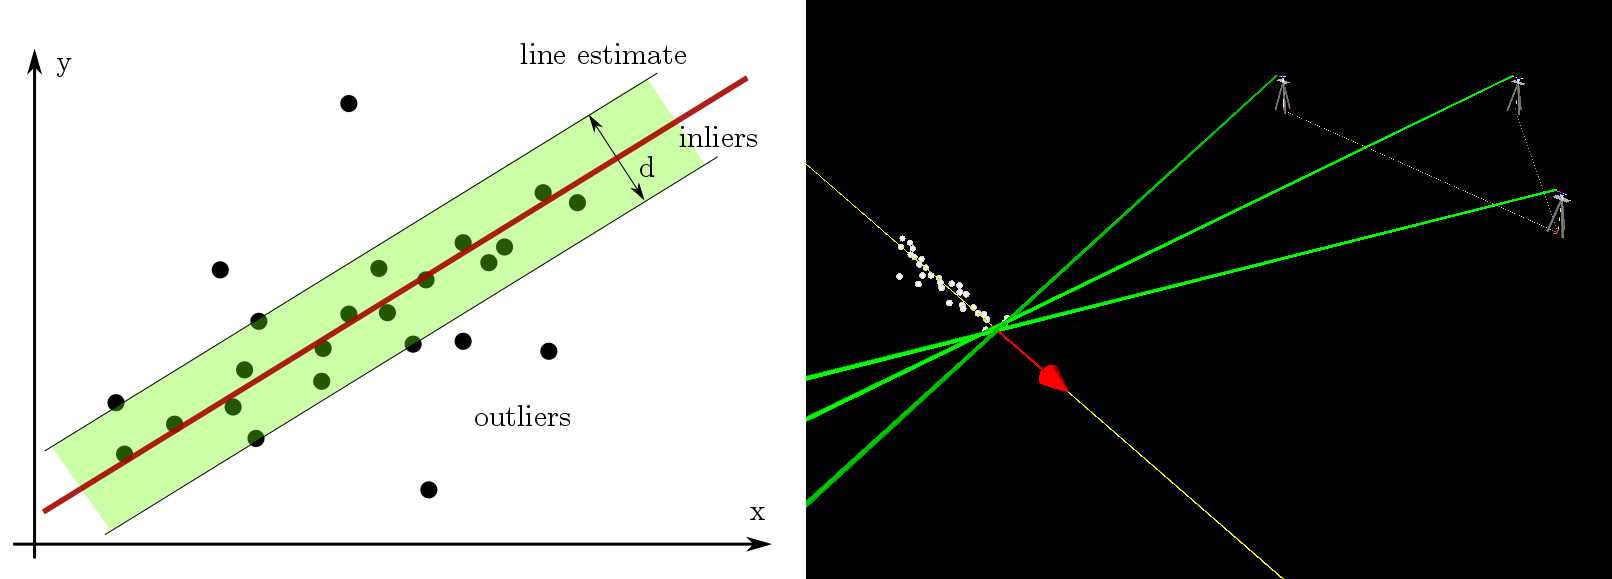
\includegraphics[width=0.8\linewidth]{fig/ransac_theory_rviz.png}
	\caption{The RANSAC algorithm is capable of estimating the model parameters given the noisy data and it is robust even in the presence of outliers which are effectively disregarded (left). This method is used in the OLS in order to estimate the direction and speed of the target with the assumption of linear motion model (right). The three-view scenario where the 3D line (yellow) is fitted to the noisy measurements (white spheres) and where the speed is estimated (red arrow) is demonstrated in \textit{rviz} environment.}
	\label{fig:ransac}
\end{figure}

%-------------------------------------------------------------------------
%-------------------------------------------------------------------------
\section{Occlusion Prediction} \label{txt:occlusion_prediction}

\todo{dokoncit}

%- zminit, ze byl testovan widely used SW VisualSFM, ale bohuzel nepodporuje inicialni vlozeni intrinsics a extrinsics pro vice kamer
%- zminit, ze je pomoci VisualSFM aspon ukazano, jaky je rozdil mezi pouzitim 2 nebo 4 (ci vice) views na rekonstrukci popelnice z gazeba.
%- zminit, ze detailni zabyvani se 3d rekonstrukci je out of scope teto prace, prace se zameruje spis na pouziti rekonstruovaneho modelu pro predikci okluze
%- popat algoritmus predikce (vypocet uhlu vektoru k danemu 3D bodu a predpovezene pozici cile)
%- dat obrazek, pohled shora, kde cil se pohybuje smerem za prekazku, zobrazit predikovanou pozici cile a vybarvit body, ktere nalezi prekazce
% zminit pozuiti PCL (odkazuji se na ni z textu sem)

%% Schema of occlusion by obstacle as seen by 2 CUs. Occlusion prediciotn via point cloud schema.
\begin{figure}[htb]
	\centering
	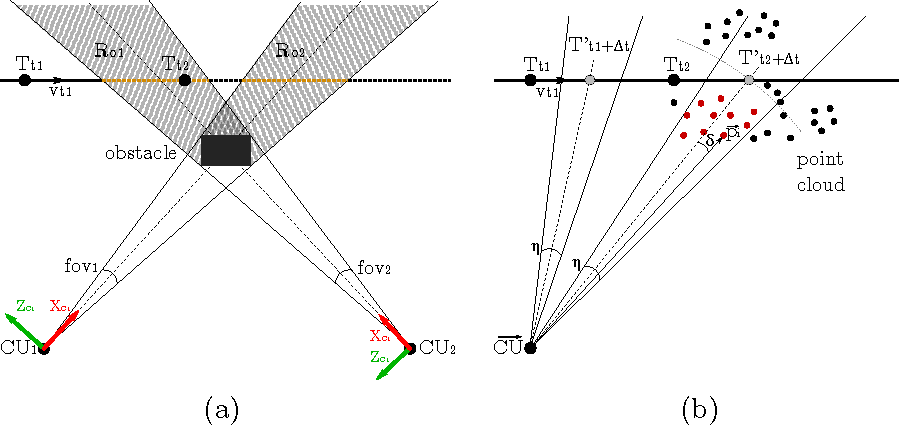
\includegraphics[width=0.95\linewidth]{fig/occlusion_2_units_pointcloud.pdf}
	\caption{\todo{pridat caption}.}
	\label{fig:occlusion_prediciton}
\end{figure}

%-------------------------------------------------------------------------
%-------------------------------------------------------------------------
\section{Hardware and Software Architecture} \label{txt:hw_and_sw_architecture}

In order to support scalability and to meet the computational demands, the OLS is designed as a distributed system where each camera unit is equipped with its own desktop computer. Sections \ref{txt:hardware_topology} and \ref{txt:components_of_cu} describe the hardware architecture of the system and internals of the camera unit. The section \ref{txt:sw_pipeline} then presents the main software pipeline from the input of the operator to the estimated position of the target in 3-space.

%.........................................................................
%.........................................................................
\subsection{Hardware Topology} \label{txt:hardware_topology}

Considering the big picture of the system, OLS is designed as a simple two layer tree topology, where each node is represented as either tracking unit or overview unit (TU/OU)~--~a~standalone independent device continuously capturing the camera image stream, performing visual tracking and regulating the motion of the manipulator. All TU/OUs are interconnected via the Gigabit Ethernet switch. 

One of the TU/OUs is selected as the \textsc{master} -- a root of the tree topology which is continuously receiving the tracking estimates from all the TU/OUs and estimating the 3D location of the target (see Figure \ref{fig:hw_ols}). Additionally, \textsc{master} serves the purpose of the interface between the OLS and the human operators and enables them to manually initialize the system and control each TU/OU (using keyboard and/or joystick) during runtime if necessary. All the TU/OUs are synchronized using PTP which is ensured by the hardware support provided by Prosilica cameras.


%% The big picture diagram of the hardware components of the OLS
\begin{figure}[htb]
	\centering
	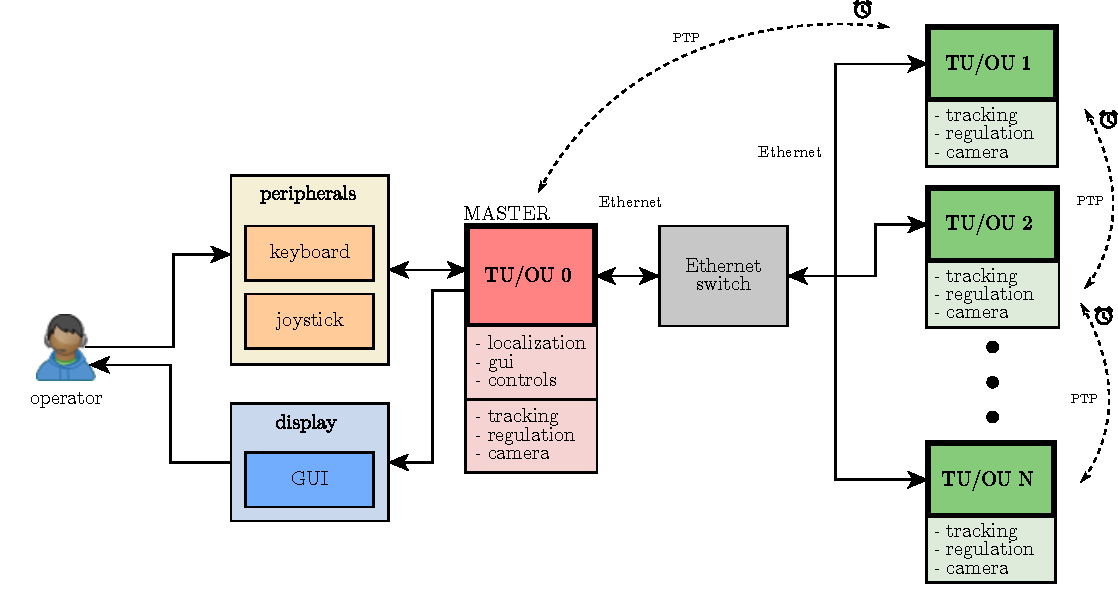
\includegraphics[width=0.9\linewidth]{fig/hwsw_architecture.pdf}
	\caption{The hardware diagram of the OLS depicting the interconnection of the main building blocks -- the tracking and/or overview units (TU/OU).}
	\label{fig:hw_ols}
\end{figure}

%.........................................................................
%.........................................................................
\subsection{Components of the Camera Unit} \label{txt:components_of_cu}

As described in \ref{txt:devices} a camera unit itself consists of a P\&T unit, a camera, sensors used for stationing and a desktop computer running the OLS software. The P\&T unit and all the sensors communicate through the RS-232 bus with the controller (based on $\mu$P STM32F4007) serving the purpose of the hub aggregating the communication with the desktop PC. The controller was designed and produced by the Department of Measurement at Faculty of Electrical Engineering, CTU in Prague. The camera is connected via GigE bus and finally the desktop computer is linked to the Ethernet Switch via Ethernet bus (see Figure \ref{fig:hw_camera_unit}).

%% The diagram of the hardware components of the camera unit
\begin{figure}[htb]
	\centering
	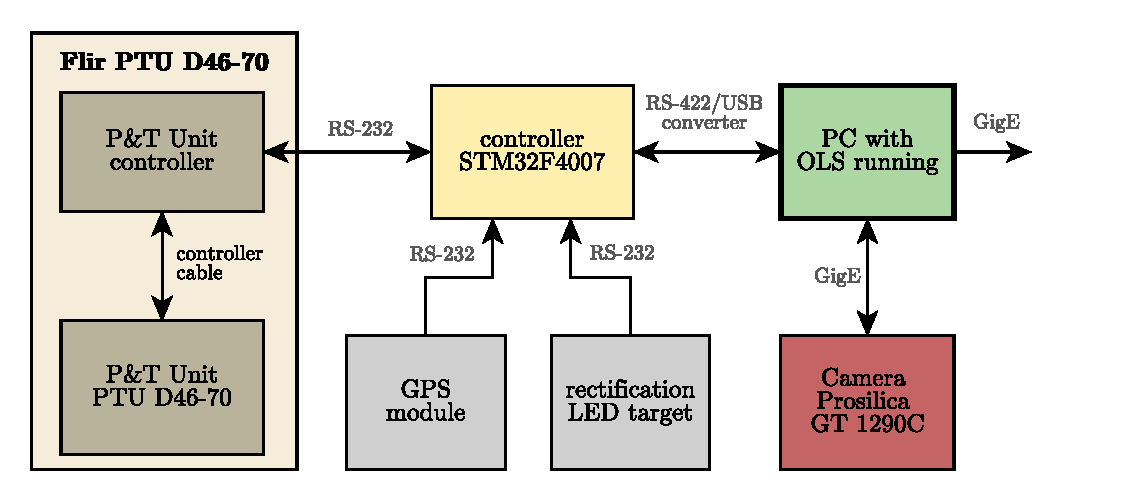
\includegraphics[width=0.8\linewidth]{fig/hw_camera_unit.pdf}
	\caption{The diagram of the hardware components of the camera unit depicting both the hardware devices and the communication standards.}
	\label{fig:hw_camera_unit}
\end{figure}

%.........................................................................
%.........................................................................
\subsection{Software Pipeline} \label{txt:sw_pipeline}

The operation of the OLS in the means of data flow is depicted in Figure \ref{fig:pipeline}. The OLS is initialized by the human operator who directs the CUs to the desired target and starts the tracking process. All the selected tracking units then visually track the target, continuously stream current measurements to the \textsc{master} and regulate the motion of the P\&T unit so that the target would not disappear from their fields of view.

The localization component continuously estimates the location of the target in 3-space given the observations from the single tracking units. Given the knowledge of the target positions history and the suitable motion model the speed and future trajectory of the target can be estimated and used in order to refine the tracking. The final estimate of the current target location is continuously emitted and presented to the operator. Should the operators decide to interfere, the peripherals (keyboard/mouse/joystick) can be used to manually adjust the tracking and regulation.

%% OLS runtime pipeline
\begin{figure}[htb]
	\centering
	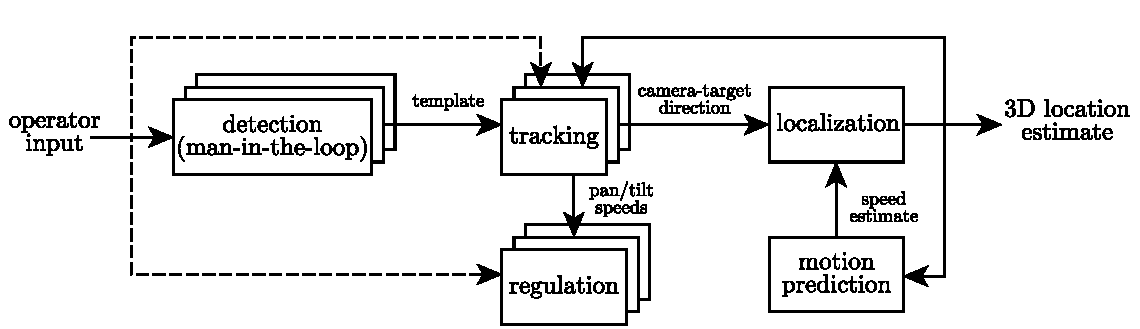
\includegraphics[width=0.95\linewidth]{fig/pipeline.pdf}
	\caption{The end-to-end pipeline of the OLS in the means of data sent among the separate software components.}
	\label{fig:pipeline}
\end{figure}


%=========================================================================
%=========================================================================
\chapter{Implementation} \label{txt:implementation}

The implementation of the OLS is built on the robotic framework \textit{Robot Operating System} and \textit{C++} is used as the main programming language. Furthermore, the physical simulator \textit{Gazebo} was used during both development and testing phase in order to prepare the system for real world environment tests. Due to the platforms support limitations of the ROS, the OLS can only be run within Linux distribution Ubuntu.

Section \ref{txt:application_of_ros} provides the reasoning for why the ROS was chosen as the base framework, Section \ref{txt:system_architecture} focuses on the architecture of the OLS, shows the user interface and summarizes the external libraries integrated in the system. Finally, Section \ref{txt:development_and_testing} demonstrates the necessity of using the simulator Gazebo and gives the technical background of how the ROS was used in order to obtain the real world environment datasets and to test the OLS.

%-------------------------------------------------------------------------
%-------------------------------------------------------------------------
\section{Application of the ROS} \label{txt:application_of_ros}

The ROS\footnote{Official website of the ROS: \url{http://www.ros.org}} is a collection of open source libraries, tools and conventions which serve the purpose of a middlewear running alongside a real operating system. Among other features the ROS provides the programmer with hardware abstraction, low-level device control, implementation of commonly-used functionality, message-passing among processes, package management, a wide range of visualization and debugging tools, time synchronization or data capture and playback \cite{O'Kane201310}.

Utilization of ROS significantly simplified the development since it provides the tools and means meeting the requirements posed by the design of the OLS (see Section \ref{txt:ros_properties_used_in_ols}). Above that, the ROS encompasses multiple packages providing common algorithms and support for hardware devices which the OLS relies on (see Section \ref{txt:standard_ros_packages}).

%.........................................................................
%.........................................................................
\subsection{ROS Properties Used in the OLS} \label{txt:ros_properties_used_in_ols}

The OLS is designed to become a relatively complex system, thus it exhibits non-trivial implementation requirements --- among others, the distribution of the running components among multiple computers, the time synchronization or fast computation of transformations among coordinate frames. Table \ref{tab:ols_requirements_ros_features} lists all the main requirements of the OLS and corresponding features of the ROS.

{\renewcommand{\arraystretch}{1.3}
	\begin{table}[!htbp]
		\centering
		\caption{The table lists the most important requirements of the OLS and describes how the ROS framework addresses them.}
		\begin{tabularx}{0.99\textwidth}{XX}
			\toprule
			\textbf{OLS requirements} & \textbf{ROS features} \\
			\midrule
			support for camera Prosilica, P\&T unit Flir PTU D46-70, joystick, keyboard & packages \texttt{avt\_vimba\_camera}, \texttt{keyboard}, \texttt{joy} \\
			distribution of computation among multiple computers & abstraction layer for distributing nodes across devices \\
			simple data exchange among subsystems & the publisher/subscriber paradigm \cite{O'Kane201310}, support for custom message formats \\
			real time performance & C++ implementation, intrinsic OS level parallelism (each node runs as a process) \\
			modeling and simulating the CUs & custom language \texttt{URDF}\footnotemark ~for robot modeling, integration with Gazebo \\
			modeling a kinematic chain, heavy 3D transformations computation & native support for computing transformation between frames using package \texttt{tf} \\
			3D visualizations & tool \texttt{rviz} for visualizing transformations, robot models, image streams etc. \\
			advanced debugging & multiple introspection tools such as \texttt{rqt\_graph}, \texttt{rqt\_tf\_tree}, \texttt{rosparam}, \texttt{rostopic}, \texttt{rosmsg} etc. \\
			physical simulation & integration with Gazebo \\
			data streams synchronization & message filters for approximate time synchronization \\
			data capturing and playback & custom container format \texttt{bag} and related tools (\texttt{rosbag}, \texttt{rqt\_bag} etc.) \\
			support for popular math and vision libraries & conversion API for easy integration of libraries OpenCV, PCL and Eigen \\
			\bottomrule
		\end{tabularx}
		\label{tab:ols_requirements_ros_features}
	\end{table}
}
	
\footnotetext{Modeling language \texttt{URDF}: \url{http://wiki.ros.org/urdf}}
	
%.........................................................................
%.........................................................................
\subsection{Standard ROS Packages Used in the OLS} \label{txt:standard_ros_packages}

ROS provides a wide range of packages for interaction with commonly used hardware devices and for performing various computations. Implementation of the OLS utilizes following packages:

\paragraph{avt\_vimba\_camera\protect\footnote{Package avt\_vimba\_camera: \url{http://wiki.ros.org/avt_vimba_camera}}}
This package wraps the Vimba GigE SDK provided by Allied Vision Technologies, the manufacturer of the Prosilica series cameras, and allows the programmer to subscribe to the topic \texttt{camera\textbackslash image\_raw} to easily access the image stream.

\paragraph{keyboard\protect\footnote{Package keyboard: \url{http://wiki.ros.org/keyboard}}}
The package processes the keyboard events and exposes them via \texttt{keydown} and \texttt{keyup} topics.

\paragraph{joy\protect\footnote{Package joy: \url{http://wiki.ros.org/joy}}}
This package processes the events from a joystick and/or gamepad and exposes them via \texttt{joy} topic.

\paragraph{tf\protect\footnote{Package tf: \url{http://wiki.ros.org/tf}}}
The package manages the distribution of the poses of all kinematic chain joints (representing the CUs) among all nodes and it computes the transformations between requested pair of frames \cite{tf}.

%-------------------------------------------------------------------------
%-------------------------------------------------------------------------
\section{System Architecture} \label{txt:system_architecture}

The OLS is divided into multiple ROS nodes with the aim to loosely resemble the hardware components. Predefined ROS messages as well as the custom ones are used to exchange the data among nodes. During runtime the operator is presented with a set of windows serving the purpose of visualizing the current state and providing the interaction capabilities. The main output of the OLS is the continuous stream of the textual information representing the estimated information about the tracked target, most importantly its global location given in UTM coordinates.

%.........................................................................
%.........................................................................
\subsection{Nodes Interaction Design} \label{txt:nodes_interaction_design}

% Five namespaces are used, one \texttt{master} namespace and four \texttt{camera\_unit\_N} namespaces, where $N \in \{0, 1, 2, 3\}$ identifies a unique camera unit. 
 
The overview of the system architecture from the perspective of the ROS namespaces, nodes, messages and services is depicted in Figure \ref{fig:sw_ols}. The distribution of the computation tasks to the separate nodes loosely corresponds to the end-to-end data flow pipeline proposed in Section \ref{txt:sw_pipeline} (see Figure \ref{fig:pipeline}). The nodes running within the \textsc{master} namespace serve the purpose of the access point for the operator as well as the main controller of the whole system while each of the namespaces \texttt{CU-N} controls a separate CU.

%% The diagram of the software components - ROS nodes - and ROS topics.
\begin{figure}[htb]
	\centering
	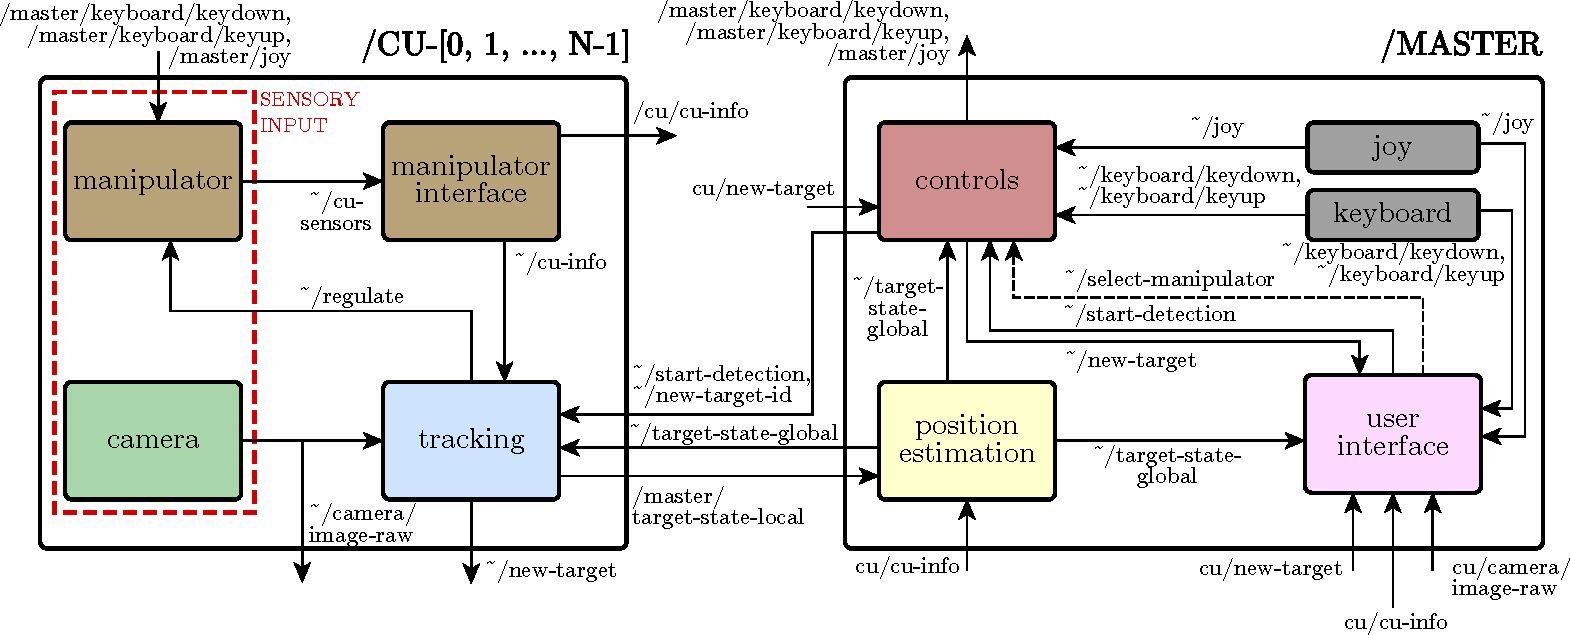
\includegraphics[width=0.98\linewidth]{fig/sw_ols.pdf}
	\caption{The diagram of the software components represented by the ROS nodes. The communication among topics is implemented using ROS messages (standard arrows) and ROS services (dashed arrows).}
	\label{fig:sw_ols}
\end{figure}

Required target is selected via the \textit{user interface} node (using either of the peripherals controlled by the \textit{joy} and \textit{keyboard} nodes) and the information is immediately propagated to the \textit{controls} node which keeps the information about all tracked targets. The \textit{tracking} node of the given CU is informed about the new target and the visual tracking is initialized. Furthermore, the \textit{tracking} node continuously regulate the motion of the P\&T unit --- the \textit{manipulator} node --- and it publishes its estimates of the target position in two-space. 

The \textit{position estimation} node continuously receives the measurements from single trackers and it computes the final estimate of the target position in three-space. Additionally, it estimates the parameters of the target motion model. Finally, the output is presented to the operator via the \textit{user interface} node and the textual data information is published via the \textit{target-state-global} message.

%.........................................................................
%.........................................................................
\subsection{User Interface}

The OLS do not provide a single integrated graphical user interface. Contrarily, the user interface is composed of multiple windows, each having a different purpose (see Figure \ref{fig:gui}). The \textit{camera\_stream} window which is opened for each CU displays the image stream from corresponding camera and allows the user to select the target of interest (by drawing a bounding box). Furthermore, it displays the progress of tracking and estimated information about the tracked target. The \textit{rviz} window displays the 3D visualization of all CUs and back-projected rays and the \textit{maps} window displays the position and orientation of all CUs and the localized target.

%% GUI
\begin{figure}[htb]
	\centering
	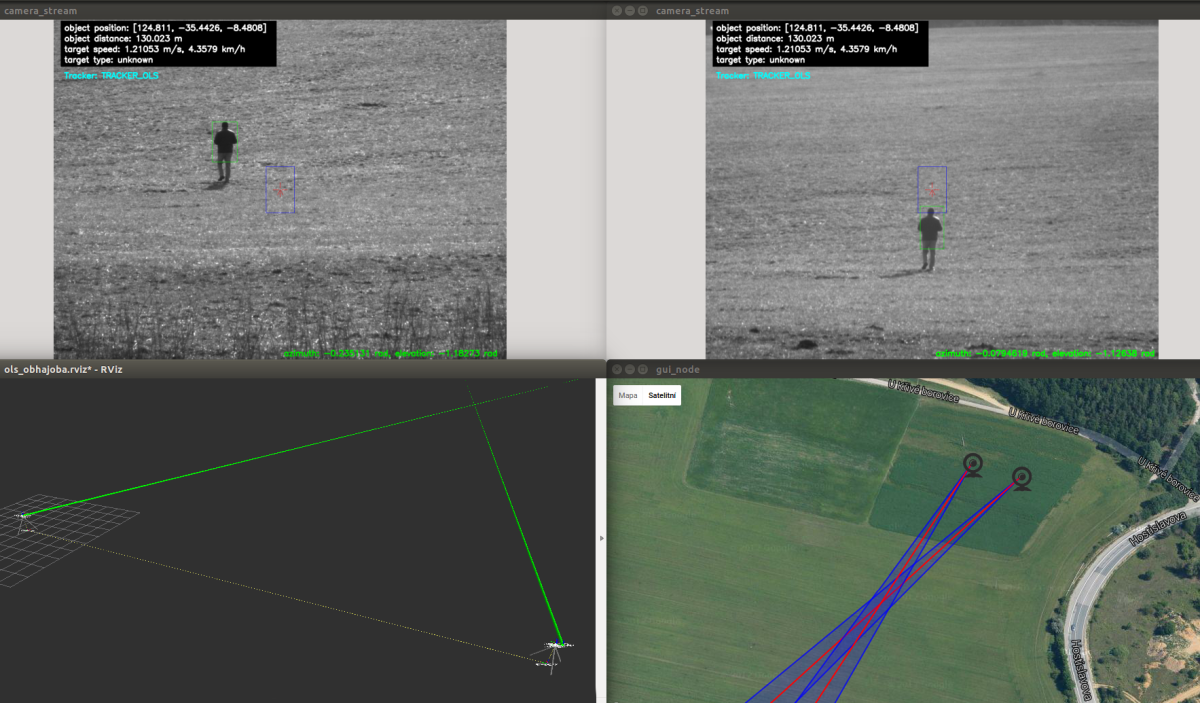
\includegraphics[width=0.85\linewidth]{fig/gui.png}
	\caption{The graphical interface of the OLS containing the \textit{camera\_stream} windows (top), \textit{rviz} window (bottom left) and \textit{maps} window (bottom right).}
	\label{fig:gui}
\end{figure}

%.........................................................................
%.........................................................................
\subsection{Third Party Software Used in the OLS} \label{txt:external_libraries}

Besides the framework ROS a few other publicly available libraries are used within the implementation:

\paragraph{OpenCV} Computer vision library\footnote{The official website of OpenCV: \url{http://opencv.org}} providing algorithms for image processing, computer vision and machine learning. Version 2.4.11 compiled with the support for CUDA is used. In the OLS it is used by both visual trackers and by the \textit{user interface} node.

\paragraph{Eigen} Open source C++ template library\footnote{The official website of Eigen: \url{http://eigen.tuxfamily.org}} implementing the data structures and methods for fast solving of linear algebra problems. The OLS uses Eigen mostly for computations regarding the triangulation.

\paragraph{PCL} An open-source library for 2D/3D image and point cloud processing\footnote{The official website of PCL: \url{http://pointclouds.org/}}. Motion prediction based on fitting the line to the scattered data using RANSAC algorithm utilizes the PCL in the OLS.

\paragraph{TLD tracker} The OpenTLD library\footnote{The official website of OpenTLD: \url{http://www.gnebehay.com/tld}} represents an open source C++ implementation the TLD tracking algorithm (see Section \ref{txt:tracking_learning_detection}).	

\paragraph{BGFG tracker} The implementation of the BGFG tracker (see Section \ref{txt:bgfg_tracker}) which was provided by the authors of the tracker \cite{ObjectTrackinginMonochromaticVideo}.

\paragraph{Serial} A cross-platform library\footnote{The official website of Serial: \url{https://github.com/wjwwood/serial}} implemented in C++ providing the API for interfacing with RS-232 serial like ports. It is used to control the P\&T unit Flir PTU D46-70.

\paragraph{LatLong-UTM} An open-source library\footnote{The official website of LatLong-UTM: \url{http://ereimer.net/programs/LatLong-UTM.htm}} providing routines for coordinate conversion between WGS84 and UTM coordinate systems.s

%-------------------------------------------------------------------------
%-------------------------------------------------------------------------
\section{Development and Testing} \label{txt:development_and_testing}

- uvod

%.........................................................................
%.........................................................................
\subsection{Application of Gazebo} \label{txt:application_of_gazebo}

Gazebo\footnote{The official website of Gazebo: \url{http://gazebosim.org}} is a physical simulator providing the tools to model and simulate robots in both indoor and outdoor environment. Since the Gazebo is distributed as one of the standard packages of the ROS framework it is straightforward to integrate the simulation environment with the already implemented ROS nodes. Since the OLS is designed to track and localize very distant targets it is not possible to test the system during development in the laboratory. Therefore, the physical simulation is necessary for the development phase in order to prepare the system for the real world operation. Gazebo was used for multiple tasks:

\paragraph{Testing the tracker} Gazebo provides the ROS plugin simulating an RGB camera which captures the virtual scene and publishes a stream of rendered images. Therefore, it can be used to test an object tracking algorithm using arbitrarily complex environment and moving objects (see Figure \ref{fig:gazebo}).

%% The screenshot of Gazebo scene and image streams from cameras.
\begin{figure}[htb]
	\centering
	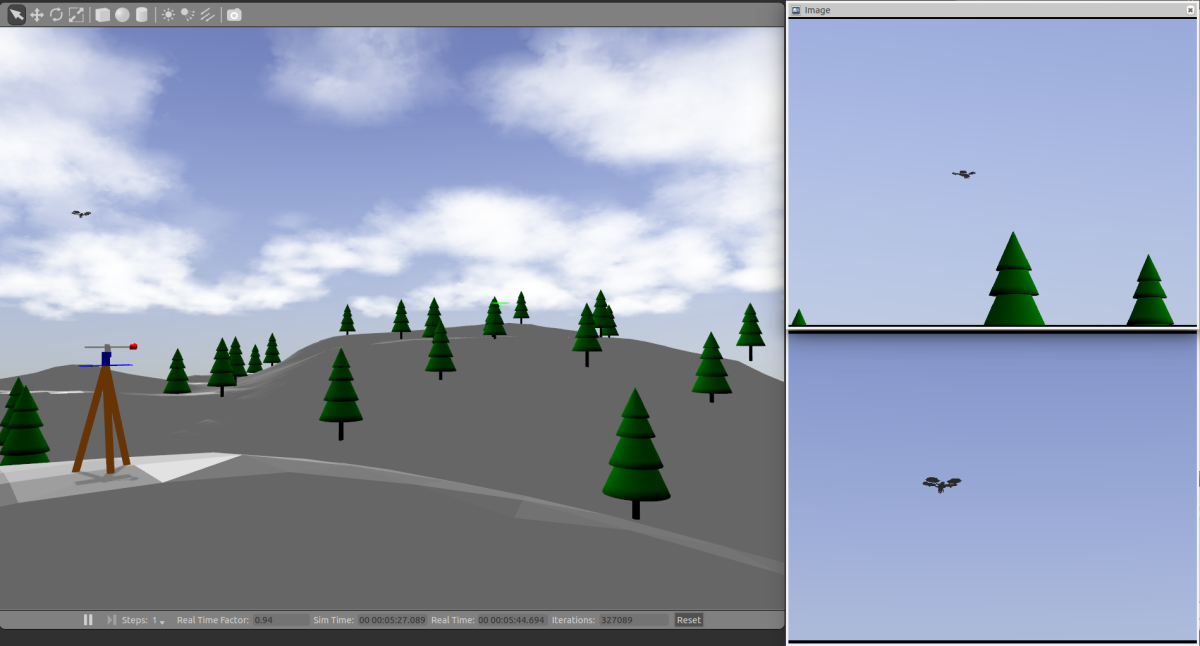
\includegraphics[width=0.65\linewidth]{fig/gazebo.png}
	\caption{The screenshot of a Gazebo simulation (left) consisting of a virtual environment (terrain with trees), a flying object (the UAV) and two CUs. Both virtual camera streams are displayed real-time using \texttt{rviz} tool (right).}
	\label{fig:gazebo}
\end{figure}

\paragraph{Testing the P\&T unit} It is a good practice to include a real hardware in the simulation during the development in the \textit{hardware-in-the-loop} manner \cite{on_hw_in_the_loop}. Both actuators and sensors would be difficult to simulate properly, moreover a real P\&T unit is constrained in terms of the operational range (see Section \ref{txt:camera_unit}), maximum acceleration and speed and communication throughput so it is necessary to thoroughly test its performance. The simulation reveals whether the implementation of motion control is correct and whether the possibilities of the P\&T unit suffice to track arbitrarily fast (simulated) objects.

\paragraph{Testing the triangulation} Thanks to the Gazebo it is possible to simulate a flying object with a-priory set trajectory (see Figure \ref{fig:gazebo}) and evaluate the precision of a position estimation algorithm using comparison between the estimated target position and a ground-truth. The visualization of the back-projected rays forming the skew-lines is done using visualization tool \textit{rviz}\footnote{The ROS package rviz: \url{http://wiki.ros.org/rviz}} (see Figure \ref{fig:rviz}).

%% Screenshot from rviz where three CUs track a target.
\begin{figure}[htb]
	\centering
	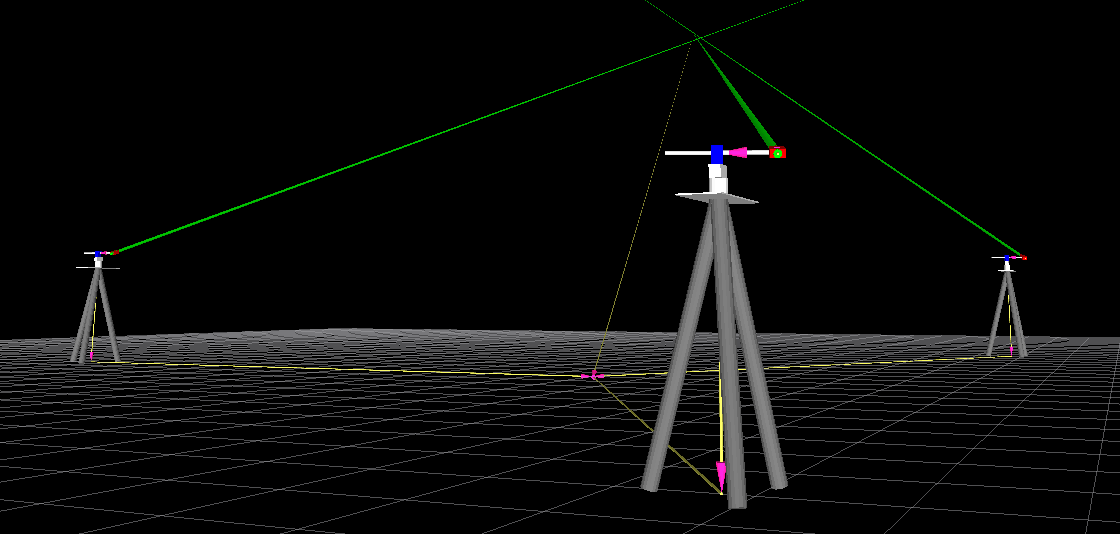
\includegraphics[width=0.65\linewidth]{fig/rviz.png}
	\caption{Three CUs tracking the target and the back-projected rays are visualized by the \textit{rviz} tool.}
	\label{fig:rviz}
\end{figure}

%.........................................................................
%.........................................................................
\subsection{Ground Truth Tracker} \label{txt:ground_truth_tracker}

Both visual trackers employed by the OLS are expected to provide noisy and delayed measurements. The noise might be caused by either of the typical tracking difficulties (see Section \ref{txt:object_tracking}) and the delay is inevitable due to the computational complexity of visual tracking algorithms. What is more, both the noise and the delay will vary across different environments and different devices running the OLS. As was explained in Section \ref{txt:precision_analysis} the random error of the visual tracker can ha sever impact on the localization precision.

Therefore, in order to test the performance of the OLS utilizing the sub-optimal visual tracking algorithm, the \textit{ground truth (GT) tracker} simulating both the noise and the delay was implemented. In time $t$ the GT tracker outputs the estimated 2D position $\vec{o_{t-t_{d}}}$ of the target $\vec{O_{t-t_{d}}}$:

\begin{align}
\vec{o_{t-t_{d}}} &= \matr{P_{t-t_{d}}}\vec{O_{t-t_{d}}} + \vec{o_{n}},\\ 
t_{d} &\sim \mathcal{N}(\mu_{t_{d}}, \sigma_{t_{d}}),\\
\vec{o_{n_{dim}}} &\sim \mathcal{N}(\mu_{n_{dim}}, \sigma_{n_{dim}}),
\end{align}
where $t_{d}$ is the time delay, $\matr{P_{t-t_{d}}}$ is the projection matrix at time $t-t_{d}$, $\vec{o_{n}}$ is the (2D) noise, $\mu_{t_{d}}$ and $\sigma_{t_{d}}$ are the parameters for the time delay normal distribution and $\mu_{n_{dim}}$ and $\sigma_{t_{dim}}$ are the parameters for the noise normal distribution for each dimension $dim$. By changing the constants $\mu_{t_{d}}$. $\sigma_{t_{d}}$, $\mu_{n_{dim}}$ and $\sigma_{n_{dim}}$ it is possible to simulate various performance of the visual tracker.

%.........................................................................
%.........................................................................
\subsection{Handling the Datasets} \label{txt:handling_datasets}

When testing the OLS in the real world environment it is necessary to record all the sensory data so that the experiments can be rerun later (with different implementations, different settings etc.). Since all the streams must be time synchronized, the time stamps must be recorded as well and the resulting dataset should be easy to playback.

For these purposes the ROS provides the data format \textit{bag}\footnote{The bag format provided by the ROS: \url{http://wiki.ros.org/Bags}} as well as the set of tools for both recording, editing and playing back the data. The OLS was designed so as to only record the sensory data coming from the P\&T unit (the \textit{manipulator} node) and the camera (the \textit{camera} node). 

Therefore, once recorded, both these nodes constituting the \textsc{sensory input} (see Figure \ref{fig:sw_ols}) can be easily replaced by the playback of the given \textit{bag} representing the recorded data. This approach makes the system operate as if it was running in the real world environment, hence various tests can be rerun repeatedly.

%=========================================================================
%=========================================================================
\chapter{Experimental Results} \label{txt:experimental_results}

The OLS was tested both in simulated and real world environment. The simulation was based on Gazebo and utilized hardware-in-the-loop approach. Section \ref{txt:test_regulation} describes the first test which compares various regulation functions and finds the most suitable parameters. Section \ref{txt:multi-camera_scenario} looks closely on the geometrical limitations of the OLS and verifies the proposed approach to localize the target using geometry based weights. Finally, Section \ref{txt:real_world_testing} explains how the real world datasets were obtained and what precision the OLS achieves.

%-------------------------------------------------------------------------
%-------------------------------------------------------------------------
\section{Regulation of the P\&T Unit Motion} \label{txt:test_regulation}

As explained in Section \ref{txt:2d_motion_prediction_and_regulation} it is desirable to keep the tracked target as close to the image center as possible by instructing the P\&T unit to rotate the camera. Furthermore, the motion should be smooth and as fast as possible, however, it should cope with the delays imposed by the visual tracker computation, the communication latency and the latency of the hardware (P\&T unit). Hardware-in-the-loop approach was taken in order to test the real P\&T unit in the simulated environment and the \textit{GT tracker} (see Section \ref{txt:implementation}) was utilized.

First, both proposed regulation functions (linear and power, see Section \ref{txt:2d_motion_prediction_and_regulation}) with various settings of parameters $a$ and $k$ were tested. In this scenario the objective was to position the camera so as to aim directly on the static target. The constants $\mu_{d} = 0.120~s, \sigma_{d} = 0.010~s, \mu_{n} = 0~px, \sigma_{n} = 0~px$ were selected for the \textit{GT tracker} to simulate the worst case delay scenario of the visual tracker performance.

As can be seen in Figure \ref{fig:test_reg_lin_pow}, the linear function cannot be too steep (high value of derivative $a$), otherwise the P\&T unit overshoots the target position and it must return (the cases of linear functions where $a = 1.0$ and $a = 5.0$) which is inadmissible behavior. Contrarily, if set correctly the power functions do not cause the overshoot and converge faster. As the result the power function with parameters $a = 2.26,~k = 1.5$ is used in the OLS.

% Comparison of different regulation functions as tested in the hardware-in-the-loop manner.
\begin{figure}[htb]\centering
	\centering
	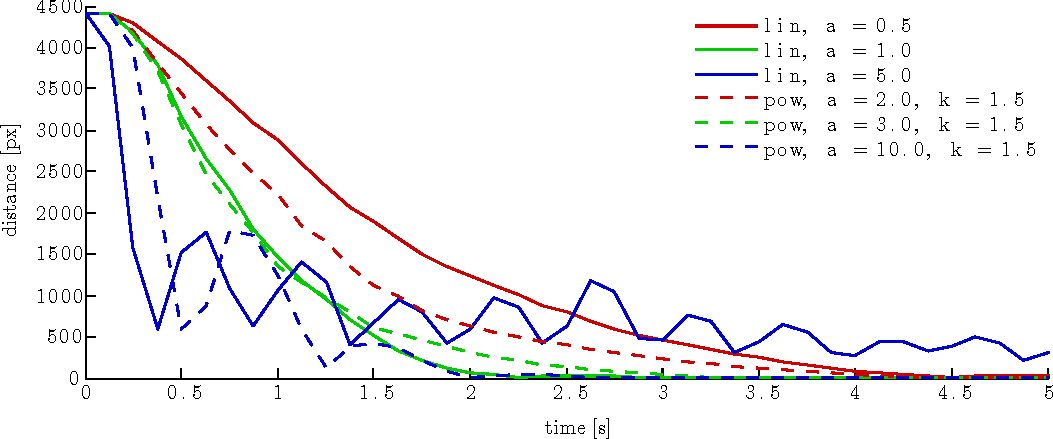
\includegraphics[width=0.75\linewidth]{fig/test_regulation_lin_pow.pdf}
	\caption{The figure depicts the Euclidean distance between the target and the center of the image plane (given in pixels) as the function of time for both linear and power regulation functions with various settings of parameters. The power function tends to converge more quickly towards the minimal distance.}
	\label{fig:test_reg_lin_pow}
\end{figure}

In order to keep the moving targets close to the center of the image plane, the prediction of future position of the target must be employed (see Section \ref{txt:2d_motion_prediction_and_regulation}). A suitable value of variable $T_{pred}$ specifying the time in the future for which the position of the target is predicted should be chosen. If $T_{pred}$ is too small the P\&T unit is not able to keep up with the motion of the target and the center of the image screen always falls behind the target. Contrarily, if $T_{pred}$ is too high, the P\&T unit overshoots to the \textit{cutoff} region (see Figure \ref{fig:regulation_lin_power}) and anticipates the position of the target.

Therefore, in the second test a simple scenario consisting of one P\&T unit and the simulated target moving with a constant speed along a line between two boundaries was created. Different values for prediction time $T_{pred}$ were set and the horizontal distance $d_{h}$ between the center of the image $PP$ and the projection $t$ of the target $T$ was measured (see Figure \ref{fig:test_motion_predict}). As was expected, with increasing value of $T_{pred}$ the overall distance $d_{h}$ decreases up to the point where the P\&T unit starts to overshoot. Note that it is not possible to select the best universal value since the performance depends on the distance, speed and motion model of the target. Therefore, it is necessary to choose the right value with regards to the given scenario.

% Comparison of amount of time for future position prediciton.
\begin{figure}[htb]\centering
	\centering
	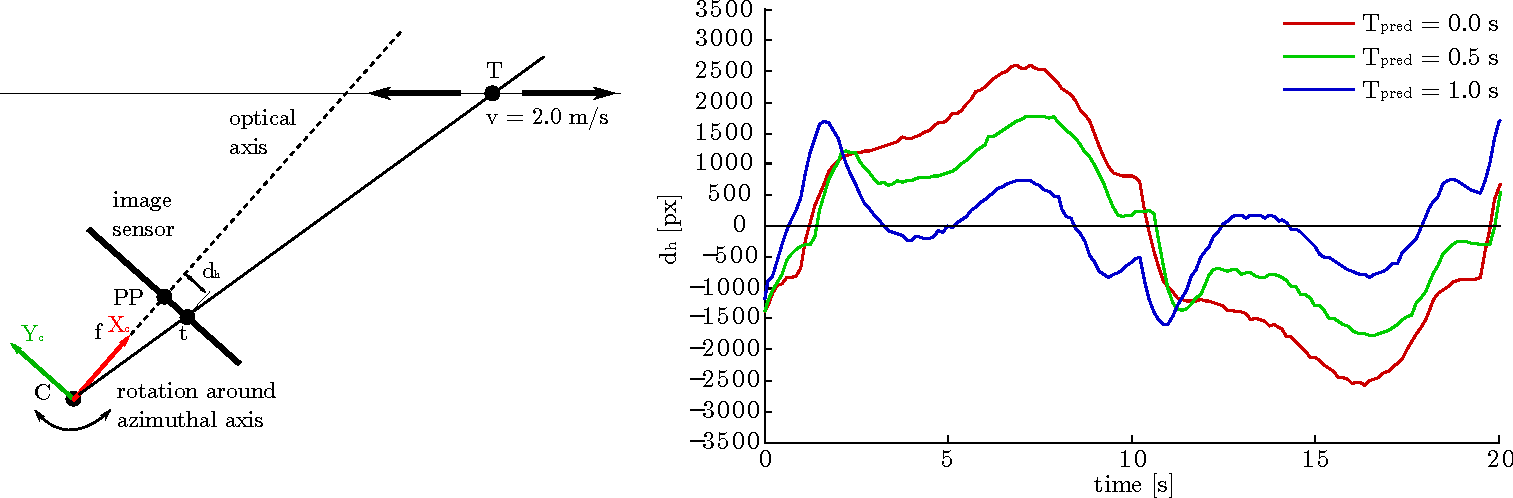
\includegraphics[width=0.95\linewidth]{fig/schema_defile_and_motion_prediction.pdf}
	\caption{Left figure depicts the schema of the perpetual linear motion of the target moving to and fro between two boundaries. Right figure shows $d_{h}$ as the function of time for different settings of prediction time $T_{pred}$.}
	\label{fig:test_motion_predict}
\end{figure}

%-------------------------------------------------------------------------
%-------------------------------------------------------------------------
\section{Multi-camera Scenario} \label{txt:multi-camera_scenario}

As was shown in Chapter \ref{txt:precision_analysis} the precision of localizing the target in 3-space significantly depends on the angle $\gamma$ between the baseline and the direction to the target. However, this geometry limitation can be alleviated by using multiple CUs which are appropriately placed within the environment so that at least one baseline which is oriented conveniently with regards to the target could always be chosen .

In order to test the proposed approach of incorporating the target-base geometry by weighting the measurements from separate baselines (see Section \ref{txt:incorporating_target-base_geometry}) two scenarios comparing the localization precision of two and three CUs were created. In both cases the goal was to localize the target moving with constant speed along the circle. In order to simulate the random error of single visual trackers, the \textit{GT tracker} with parameters $\mu_{d} = 0.120~s,~\sigma_{d} = 0.010~s,~\mu_{n} = 0~px,~\sigma_{n} = 15~px$ was used. 

In the first scenario only two CUs ($CU_{1}$, $CU_{2}$) are used and thus there are two critical regions $CR_{1}$ and $CR_{2}$ along the baseline within which the localization error is expected to be high. In the second scenario the third $CU_{3}$ was added so that all three CUs would form a regular triangle. It was expected that both critical regions would be covered by two newly created baselines. As can be seen in Figure \ref{fig:test_two_vs_three_cus} the expectations were met.

% Schema of testing two vs three units and plot with error results.
\begin{figure}[htb]\centering
	\centering
	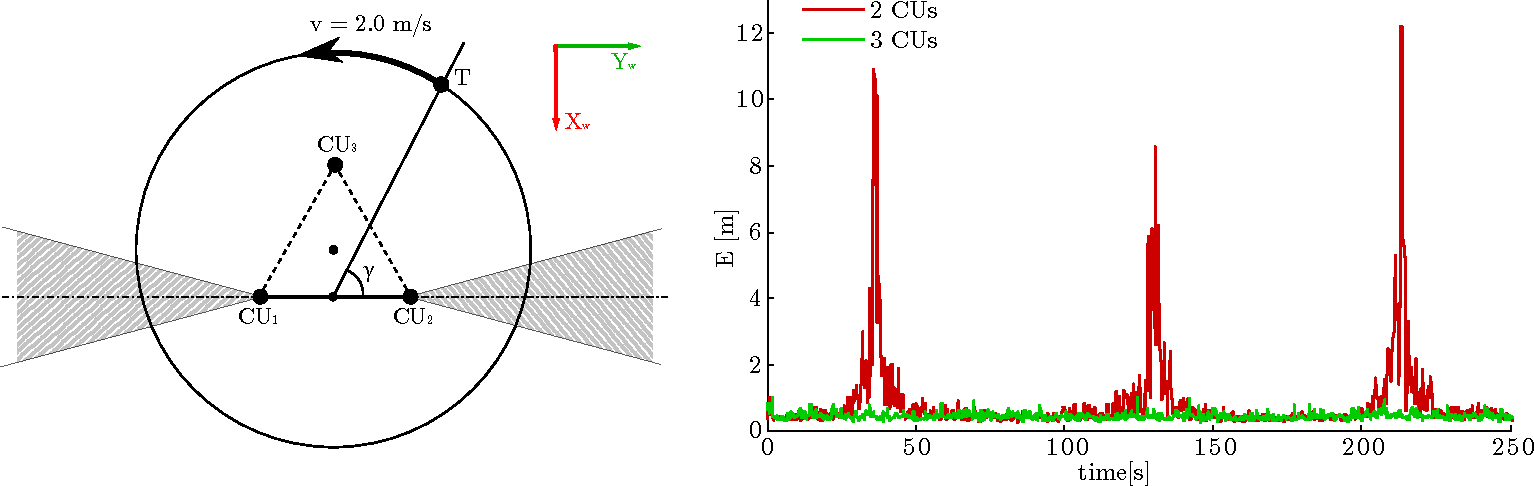
\includegraphics[width=0.95\linewidth]{fig/schema_two_vs_three_units_and_plot.pdf}
	\caption{The figure to the left depicts the schematic view of two test scenarios where either two or three CUs are used. The target $T$ moves along the circle with constant speed in the height of $2~m$. The figure to the right depicts the localization error $E$ as the function of time for both scenarios. It can be seen that in the two-camera scenario the error $E$ increases rapidly once the target reaches either of the critical regions $CR_{1}$ and $CR_{2}$.}
	\label{fig:test_two_vs_three_cus}
\end{figure}
	
%-------------------------------------------------------------------------
%-------------------------------------------------------------------------
\section{Real World Testing} \label{txt:real_world_testing}

In order to test the real world performance of the OLS two datasets were created using a basic two-camera setup. The first dataset (\textsc{meadow}) was obtained on the meadow located between districts Bystrc and Žebětín (Brno, Czech Republic). The CUs were precisely positioned using differential GPS sensor so that the baseline would be $30~m$ long. To create the second dataset (\textsc{pitch}) the athletics stadium VUT SAPPV located in district Královo Pole (Brno, Czech Republic) was chosen since the DGPS sensor was no longer available and thus the marks measuring the distance painted on the running pitch were used to station the CUs which were placed $10~m$ apart (see Figure~\ref{fig:dataset_zebetin_vut}) and presumably in the same altitude.

In both datasets the local heading was estimated by aiming the units on each other as explained in Section \ref{txt:stationing} and the global heading was computed as the rotation of the baseline with regards to the UTM coordinate frame. Standalone digital inclinometer was used to level both stations by manually adjusting the lengths of surveying tripod legs.

%% Google Earth view on the setups in Zebetin and on VUT pitch.
\begin{figure}[htb]\centering
	\centering
	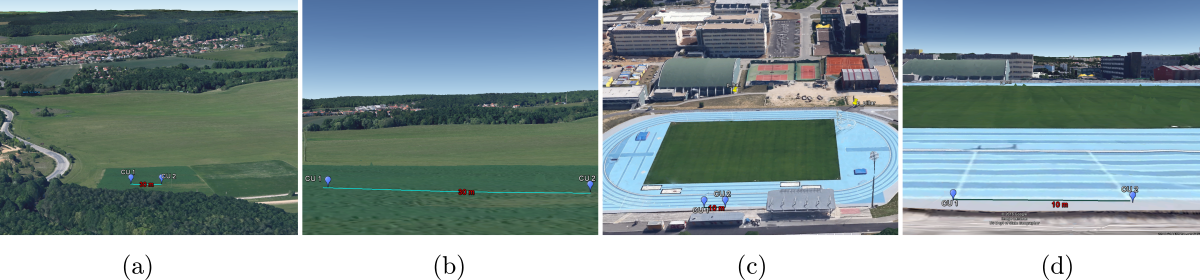
\includegraphics[width=0.98\linewidth]{fig/dataset_zebetin_vut.png}
	\caption{The overview and close-up look on the environments within which the \textsc{meadow} ((a), (b)) and \textsc{pitch} ((c), (d)) datasets were created. The geographical positions of both CUs are denoted by the blue pinpoints.}
	\label{fig:dataset_zebetin_vut}
\end{figure}

%.........................................................................
%.........................................................................
\subsection{Setup and Methodology} \label{txt:setup_and_methodology}

The system was tested in two different real-world environments and a basic two-camera setup was used in both cases. The first testing was performed on a meadow (\textsc{meadow} dataset) and the second one on the running pitch (\textsc{pitch} dataset). Multiple static targets corresponding to the visually significant landmarks were chosen so that it would be possible to find their precise geographical coordinates using the cadastral map. In case of \textsc{meadow} dataset, a moving target equipped with the handheld GPS sensor was tracked and localized as well. During all measurements only horizontal position (i.e. northing and easting parameters of the UTM coordinate frame) was considered.

For each target, the expected \textit{localization error} $E_{est}$ was computed based on the theory presented in chapter \ref{txt:precision_of_the_localization} and it was compared to the real measured error. Note that the \textit{localization error} $E_{meas}$ is defined as the Euclidean distance between the estimated and ground truth geographical location of the given target given in UTM coordinates:

\begin{align}
	E_{meas} = \sqrt{(e_{gt} - e_{e})^{2} + (n_{gt} - n_{e})^{2}}
\end{align}
where $n$ and $e$ are the northing and easting coordinates and subscripts $gt$ and $e$ denote the ground truth and the estimate.

%.........................................................................
%.........................................................................
\subsection{Static Targets}

Nine landmarks in case of \textsc{meadow} dataset and three landmarks in case of \textsc{pitch} dataset were selected to test localization. Tables \ref{tab:static_targets_zebetin} and \ref{tab:static_targets_vut_pitch} summarize ground truth and measured UTM coordinates of the targets as well as the position of the targets with regards to the baseline (angle $\gamma$ and distance $d$) which influences the total localization error (see Section~\ref{txt:precision_of_the_localization}). 

Note that due to the fact the angle $\gamma$ (see Figure \ref{fig:target-base_and_weighted_centroid}) do not vary much the overall estimated error $E_{est}$ is mainly influenced by the distance of the target $d$ which varies significantly. Therefore the targets are sorted in ascending order with respect to the distance $d$. The estimated error $E_{est}$ was calculated with assumption of the random error worth $p = 4~px$ (see Section \ref{txt:precision_of_the_localization}). 

%% Static targets Zebetin.
\begin{table}[!h]
	\centering
	\caption{The results achieved for \textsc{meadow} dataset.}
	\begin{tabular}{crrcccc}
		\toprule
		\multirow{2}[0]{*}{\textbf{object}} & \multicolumn{1}{c}{\textbf{GT pos.}} & \multicolumn{1}{c}{\textbf{estim. pos. }} & \textbf{$d$} & \textbf{$\gamma$} & \textbf{$E_{est}$} & \textbf{$E_{meas}$} \\
		\textbf{} & \multicolumn{1}{c}{\textbf{[UTM]}} & \multicolumn{1}{c}{\textbf{[UTM]}} & \textbf{[m]} & \textbf{[$\circ$]} & \textbf{[m]} & \textbf{[m]} \\
		\midrule
		\multirow{2}[0]{*}{\textbf{pillar1}} & \multicolumn{1}{l}{x: 608696.2} & \multicolumn{1}{l}{x: 608695.05} & \multirow{2}[0]{*}{91.92} & \multirow{2}[0]{*}{68.40} & \multirow{2}[0]{*}{0.20} & \multirow{2}[0]{*}{4.41} \\
		& \multicolumn{1}{l}{y: 5452998} & \multicolumn{1}{l}{y: 5452993.74} &       &       &       &  \\
		\multirow{2}[0]{*}{\textbf{pillar2}} & \multicolumn{1}{l}{x: 608714.13} & \multicolumn{1}{l}{x: 608711.56} & \multirow{2}[0]{*}{199.14} & \multirow{2}[0]{*}{63.91} & \multirow{2}[0]{*}{0.95} & \multirow{2}[0]{*}{5.51} \\
		& \multicolumn{1}{l}{y: 5452890.03} & \multicolumn{1}{l}{y: 5452885.16} &       &       &       &  \\
		\multirow{2}[0]{*}{\textbf{pillar3}} & \multicolumn{1}{l}{x: 608728.93} & \multicolumn{1}{l}{x: 608731.78} & \multirow{2}[0]{*}{285.01} & \multirow{2}[0]{*}{62.62} & \multirow{2}[0]{*}{1.93} & \multirow{2}[0]{*}{11.73} \\
		& \multicolumn{1}{l}{y: 5452804.81} & \multicolumn{1}{l}{y: 5452793.43} &       &       &       &  \\
		\multirow{2}[0]{*}{\textbf{pillar4}} & \multicolumn{1}{l}{x: 608713.61} & \multicolumn{1}{l}{x: 608720.62} & \multirow{2}[0]{*}{386.81} & \multirow{2}[0]{*}{66.61} & \multirow{2}[0]{*}{3.39} & \multirow{2}[0]{*}{17.16} \\
		& \multicolumn{1}{l}{y: 5452702.31} & \multicolumn{1}{l}{y: 5452686.65} &       &       &       &  \\
		\multirow{2}[0]{*}{\textbf{tree1}} & \multicolumn{1}{l}{x: 608687.5} & \multicolumn{1}{l}{x: 608684.5} & \multirow{2}[0]{*}{433.88} & \multirow{2}[0]{*}{70.31} & \multirow{2}[0]{*}{4.13} & \multirow{2}[0]{*}{17.20} \\
		& \multicolumn{1}{l}{y: 5452655.72} & \multicolumn{1}{l}{y: 5452652.72} &       &       &       &  \\
		\multirow{2}[0]{*}{\textbf{person}} & \multicolumn{1}{l}{x: 608481.06} & \multicolumn{1}{l}{x: 608473.64} & \multirow{2}[0]{*}{479.96} & \multirow{2}[0]{*}{84.09} & \multirow{2}[0]{*}{4.65} & \multirow{2}[0]{*}{23.90} \\
		& \multicolumn{1}{l}{y: 5452666.47} & \multicolumn{1}{l}{y: 5452643.75} &       &       &       &  \\
		\multirow{2}[0]{*}{\textbf{hide}} & \multicolumn{1}{l}{x: 608226.71} & \multicolumn{1}{l}{x: 608216.86} & \multirow{2}[0]{*}{526.86} & \multirow{2}[0]{*}{45.63} & \multirow{2}[0]{*}{7.57} & \multirow{2}[0]{*}{22.77} \\
		& \multicolumn{1}{l}{y: 5452875.99} & \multicolumn{1}{l}{y: 5452880.58} &       &       &       &  \\
		\multirow{2}[0]{*}{\textbf{tree2}} & \multicolumn{1}{l}{x: 608283.11} & \multicolumn{1}{l}{x: 608287.11} & \multirow{2}[0]{*}{634.46} & \multirow{2}[0]{*}{69.77} & \multirow{2}[0]{*}{8.56} & \multirow{2}[0]{*}{28.33} \\
		& \multicolumn{1}{l}{y: 5452618.41} & \multicolumn{1}{l}{y: 5452622.41} &       &       &       &  \\
		\multirow{2}[0]{*}{\textbf{mast}} & \multicolumn{1}{l}{x: 607816.03} & \multicolumn{1}{l}{x: 607826.83} & \multirow{2}[0]{*}{1379.67} & \multirow{2}[0]{*}{70.88} & \multirow{2}[0]{*}{41.24} & \multirow{2}[0]{*}{34.21} \\
		& \multicolumn{1}{l}{y: 5452037} & \multicolumn{1}{l}{y: 5452069.46} &       &       &       &  \\
		\bottomrule
	\end{tabular}
	\label{tab:static_targets_zebetin}
\end{table}


%% Static targets VUT pitch.
\begin{table}[!h]
	\centering
	\caption{The results achieved for \textsc{pitch} dataset.}
	\begin{tabular}{crrcccc}
		\toprule
		\multirow{2}[0]{*}{\textbf{object}} & \multicolumn{1}{c}{\textbf{GT pos.}} & \multicolumn{1}{c}{\textbf{estim. pos. }} & \textbf{$d$} & \textbf{$\gamma$} & \textbf{$E_{est}$} & \textbf{$E_{meas}$} \\
		\textbf{} & \multicolumn{1}{c}{\textbf{[UTM]}} & \multicolumn{1}{c}{\textbf{[UTM]}} & \textbf{[m]} & \textbf{[$\circ$]} & \textbf{[m]} & \textbf{[m]} \\
		\midrule
		\multirow{2}[0]{*}{\textbf{pillar}} & \multicolumn{1}{l}{x: 614563.07} & \multicolumn{1}{l}{x: 614556.08} & \multirow{2}[0]{*}{125.54} & \multirow{2}[0]{*}{52.93} & \multirow{2}[0]{*}{1.14} & \multirow{2}[0]{*}{7.77} \\
		& \multicolumn{1}{l}{y: 5453706.81} & \multicolumn{1}{l}{y: 5453703.41} &       &       &       &  \\
		\multirow{2}[0]{*}{\textbf{hall}} & \multicolumn{1}{l}{x: 614554.47} & \multicolumn{1}{l}{x: 614547.67} & \multirow{2}[0]{*}{128.91} & \multirow{2}[0]{*}{85.96} & \multirow{2}[0]{*}{1.01} & \multirow{2}[0]{*}{9.41} \\
		& \multicolumn{1}{l}{y: 5453794.96} & \multicolumn{1}{l}{y: 5453788.45} &       &       &       &  \\
		\multirow{2}[0]{*}{\textbf{fsi}} & \multicolumn{1}{l}{x: 614840.64} & \multicolumn{1}{l}{x: 614752.41} & \multirow{2}[0]{*}{425.53} & \multirow{2}[0]{*}{44.38} & \multirow{2}[0]{*}{15.80} & \multirow{2}[0]{*}{89.46} \\
		& \multicolumn{1}{l}{y: 5453589.38} & \multicolumn{1}{l}{y: 5453604.15} &       &       &       &  \\
		\bottomrule
	\end{tabular}
	\label{tab:static_targets_vut_pitch}
\end{table}

Figure \ref{fig:plot_error_estatic_targets} compares the estimated and measured localization error. Note that both $E_{est}$ and $E_{meas}$ follow the same trend of increasing value with increasing distance of the target from the baseline which is expected behavior caused by the phenomenon of diminishing accuracy of depth measurement (see Section \ref{txt:precision_of_the_localization}). 

\begin{figure}[htb]\centering
	\centering
	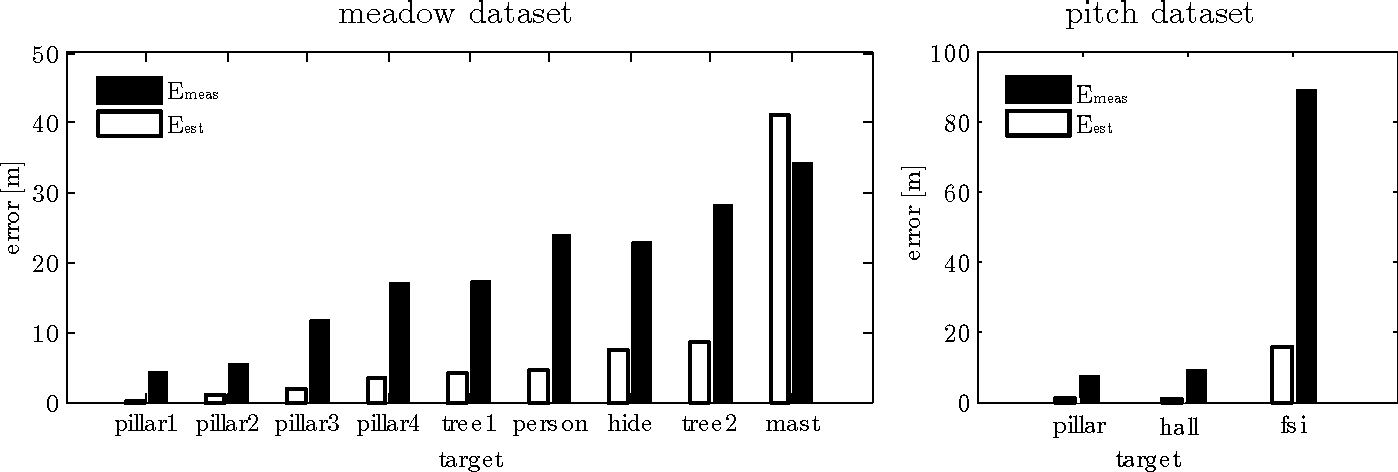
\includegraphics[width=0.98\linewidth]{fig/plot_static_targets.pdf}
	\caption{The plot displays both measured $E_{meas}$ and estimated $E_{est}$ localization error for all static targets, which are sorted in ascending order with respect to the distance (and consequently estimated error $E_{est}$).}
	\label{fig:plot_error_estatic_targets}
\end{figure}

As for the \textsc{meadow} dataset the achieved precision is approximately 4--5 times worse than expected ranging from 4.41 to 34.21 $m$. Note that the targets were selected manually in the images, hence the random error plays insignificantly small role in the total imprecision. The main source of the deflections is the systematic error caused by both imprecise rectification and stationing. 

In case of \textsc{pitch} dataset the achieved precision is approximately 6--10 times worse than expected ranging from 7.77 to 89.46 $m$. The impact of the systematic error is even greater. One of the reason is the fact the CUs were not stationed using GPS, contrarily their geographical positions were estimated by finding the pitch marks (on which the CUs were placed) on the ortophotomap. It has been noted that all the wrong estimations tended to be placed in more less correct direction, however too close to the baseline which is another clue which points to the systematic error (i.e. the mounting of the cameras might have moved slightly during the transportations).

\paragraph{Conclusion} In order to achieve higher precision more thorough elimination of systematic error must be performed. In case of rectification the human error as well as non-robust construction of the camera mounting is the main limitation (see Section \ref{txt:rectification}). In case of stationing more robust approach to leveling the stations as well as estimating the heading should be taken.

%.........................................................................
%.........................................................................
\subsection{Dynamic Targets}

In case of \textsc{meadow} dataset the system was tested against one dynamic terrestrial target equipped with a mobile GPS sensor -- a walking person (see Figure~ \ref{fig:trackingAndMap}). The target was tracked for $120~s$ and the estimated positions were captured and compared to the ground truth path (see Figure \ref{fig:resultsWalking}). On average the system achieved the precision of $6.25~m$. Note that the position estimates oscillate around the ground truth trajectory, which is caused by the random error made by both trackers; the error, however, keeps in the specific range and reaches maximum of $13.35~m$. The mean error is higher as compared to the estimated error (see Section \ref{txt:precision_of_the_localization}), which is again caused by the systematic error (imprecise rectification and stationing).

\begin{figure}[!h]\centering
	\centering
	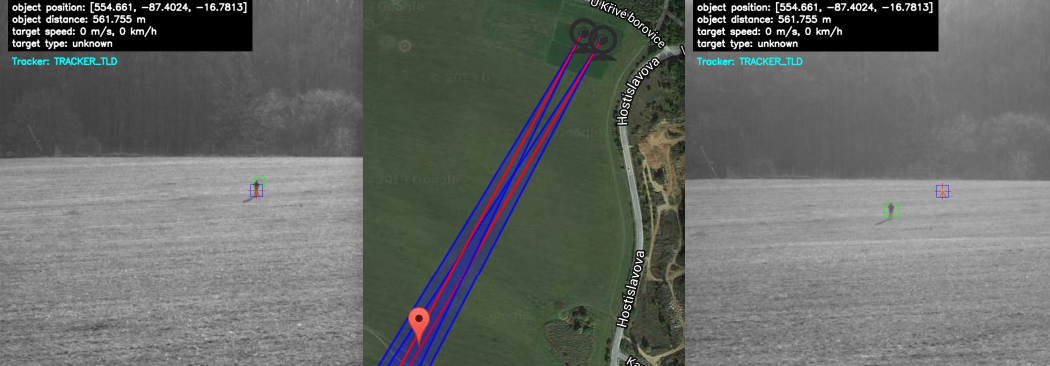
\includegraphics[width=0.98\linewidth]{fig/tracking_and_map.png}
	\caption{The two-camera setup where the distant target is tracked by both CUs (left and right). The estimated position of the target is displayed in the map (center).}
	\label{fig:trackingAndMap}
\end{figure}

\begin{figure}[htb]\centering
	\centering
	\includegraphics[width=0.44\linewidth]{fig/eval_walking.png}
	\includegraphics[width=0.54\linewidth]{fig/eval_walking_error.pdf}
	\caption{The comparison of the ground truth and estimated trajectory of a target moving in the distance range of ca $50$--$200~m$ (left). The error as the function of the distance of the target is also displayed (right). The system makes the average error of $6.25~m$.}
	\label{fig:resultsWalking}
\end{figure}

An attempt was made to localize another moving target in \textsc{pitch} dataset as well, however, it was not possible to evaluate the precision since the visual tracker was not able to follow the target properly. The main reason for faulty operation was the cluttered background of the target which prevented the tracking subsystem from providing correct measurements.

\paragraph{Conclusion} Precision of localization of the dynamic target is limited in the same way as in case of static targets. Above that, the system greatly depends on the precision of the visual tracker which should be investigated more in order to avoid incorrect measurements.

%=========================================================================
%=========================================================================
\chapter{Conclusion} \label{txt:conclusion}

A novel system for autonomous optical localization of arbitrary distant targets was presented in this work. The system is based on the visual tracking and mutli-view triangulation approaches. Triangulation is well known and widely used approach, however, the main contribution of the system is its semi-autonomous operation based on mere visual clues as opposed to the actively radiating solutions such as radars.

First, the existing state-of-the-art approaches to visual tracking were summarized and two techniques, the TLD tracker and BGFG tracker, were selected to be incorporated in the OLS. Then the problematics of multi-view triangulation was discussed and the approaches used to reconstruct the 3D environment which could be used as the base for occlusion prediction were discussed.

Thorough precision analysis was performed so as to pinpoint the most severe sources of the error. The geometrical limitations of the OLS were demonstrated and the merits of multiple-view setup over the stereo setup in the means of localization precision were shown. The stationing and rectification procedures aiming on eliminating the systematic error were then proposed. 

The model of the camera unit based on the kinematic chain was then proposed. In order to minimize the impact of the random error the BGFG tracker was adjusted so as to estimate the belief of each measurement and to include the information from frame differencing. Suitable functions for regulating the motion of the P\&T unit were discussed and the approach to triangulate the target position with the knowledge of trackers' belief and target-base geometry was proposed.

The OLS was implemented in C++ within the framework ROS. Additionally, the physical simulator Gazebo was used in both development and testing phase. The OLS was first tested using Gazebo in the hardware-in-the-loop manner. Next, two datasets were obtained in the real world environment and the system was tested against both static and moving targets. It has been shown that the localization precision is 4-10 times lower than expected while most likely culprit is the imprecisely performed stationing and rectification.

There are multiple possibilities of what to focus on in further development. The tracking algorithm should be investigated so that it would perform well even with cluttered background. More thorough stationing and rectification should be performed so as to verify the main source of imprecise localization was the systematic error. Furthermore, automatic detection and possibly classification of moving targets could be implemented and the approach to handoff the target among separate CUs should be proposed to make the OLS fully autonomous.